\documentclass[a4paper,12pt,twoside,openright]{report}

\usepackage[hmarginratio=2:3]{geometry}
\usepackage[utf8]{inputenc} % Allows using accents instead of \'.
\usepackage[spanish]{babel} % Spanish as default language.
\usepackage{graphicx}
\usepackage{tikz} % For drawing graphics.
\usepackage{amsfonts}
\usepackage{amsmath}
\usepackage{enumerate}
\usepackage{hyperref}
\usepackage{courier} % Use Courier New as monospace font.
\usepackage{palatino} % Use the Palatino font.
\usepackage{listings}
\usepackage{float}
\usepackage{paralist}
\usepackage{fancyhdr}
\usepackage{tocloft} % ToC styling.
\usepackage[backend=biber,url=false,style=numeric]{biblatex}


% Header setup.
\pagestyle{fancy}

\renewcommand{\chaptermark}[1]{\markboth{\MakeUppercase{\thechapter.\ #1}}{}}
\renewcommand{\sectionmark}[1]{\markright{\thesection.\ #1}}

\fancyhf{}
\fancyhead[RO,LE]{\thepage}
\fancyhead[LO]{\leftmark}
\fancyhead[RE]{\rightmark}


\addbibresource{mendeley-bib.bib}
%% \addbibresource{bibliography.bib}

\setlength{\parskip}{\baselineskip} % Skip a line between paragarphs.

\newcommand{\HRule}{\rule{\linewidth}{0.3mm}}

\lstset{
  language=Python,
  keywordstyle=\color{blue}\bfseries,
  commentstyle=\color{gray},
  basicstyle=\small\ttfamily,
  showstringspaces=false
}

\renewcommand{\abstractname}{Resumen} % Nombre de la sección del abstract.

\begin{document}

\begin{titlepage}
  \begin{center}

    % Upper part of the page
    \textsc{\LARGE}\\[1.0cm]
    \textsc{\LARGE Proyecto de Grado}\\[1.5cm]

    \textsc{\Large Instituto de Computación}\\[0.2cm]
    \textsc{\Large Facultad de Ingeniería}\\[0.2cm]
    \textsc{\Large Universidad de la República}\\[2.0cm]

    % Title
    \HRule\\[0.6cm]
    {\Huge \bfseries Representación de Palabras en Espacios de Vectores}\\[0.3cm]
    \HRule\\[2.3cm]

    % Authors
    {\Large Agustín \textsc{Azzinnari}} {\small (aazzinnari@gmail.com)}\\
    {\Large Alejandro \textsc{Martínez}} {\small (ale.martinez.uy@gmail.com)}\\[2.0cm]

    % Supervisors
    {\small Tutores:}\\
    {\normalsize Mathias Etcheverry}\\
    {\normalsize Dina Wonsever}\\[1.5cm]

    Mayo de 2016\\

    \vfill
    % Bottom of the page

  \end{center}
\end{titlepage}

\begin{abstract}
abstract
\end{abstract}

\tableofcontents

\chapter{Introducción}

El tratamiento de lenguaje natural (PLN) por parte de computadoras ha sido siempre un punto de gran
interés de la comunidad. Desde los trabajos de John McCarthy y Marvin Minsky en los años 1950 hasta
la actualidad, se han publicado miles de trabajos al respecto. Históricamente han habido dos
paradigmas para el tratamiento del lenguaje: uno basado en reglas y otro en aprendizaje automático.

El primer enfoque busca construir reglas que capturen el conocimiento de expertos en lingüística
para resolver una problemática particular, construyendo reglas que generalicen lo suficiente pero
sin dejar de lado los casos particulares. Mientras que ambos enfoques se desarrollaron
paralelamente, no fue hasta la adopción masiva de Internet, junto con los inmensos volúmenes de
texto que consecuentemente se generaron, que los métodos de aprendizaje automático comenzaron a ser
significativemente más exitosos.

Todas las tareas en el área de PLN involucran, en algún nivel, trabajar con palabras. Puesto que los
algoritmos de aprendizaje automático comúnmente utilizados como soluciones de dichas tareas se
alimentan de vectores, es usual requerir de un mecanismo para traducir de unas a otros.

La forma más simple de realizar esta traducción es posiblemente asociarle, a cada palabra, un vector
bajo un esquema \textit{one-hot}: esto es, a cada palabra se le asigna un vector donde todas las
componentes son cero salvo por un uno en la correspondiente a la palabra. Sin embargo, dado que
todos los vectores resultan equidistantes, esta representación no tiene la capacidad de generalizar
bien: las palabras \textit{el} y \textit{lenguaje} están a la misma distancia que \textit{el} y
\textit{de}, por lo que se pierde información de su función sintáctica y semántica. Por esta razón,
la búsqueda de métodos que asignen representaciones parecidas a palabras relacionadas es un área de
investigación de particular interés.

Basándose en la hipótesis distribucional de Harris~\cite{Harris1954}, la cual plantea que palabras
que ocurren en contextos similares tienen significados similares, se han desarrollado históricamente
una gran cantidad de métodos para realizar la tarea de traducción, principalmente basados en
construir una matriz de coocurrencias la cual asocia, a cada par de palabras del vocabulario, una
medida de similitud obtenida a partir de los contextos en los cuales éstas aparecen juntas. Estos
métodos, donde entran técnicas como el análisis semántico latente (LSA), logran resultados
relativamente satisfactorios.

Sin embargo, recientemente han surgido una nueva generación de métodos para representar palabras
que, mediante el uso de técnicas inspiradas en el modelado de lenguaje mediante redes neuronales,
han llegado resultados sorprendentes para la comunidad del PLN\@. Estos algoritmos se basan en métodos
de aprendizaje automático no supervisado que, a partir de grandes volúmenes de texto, consiguen
representaciones vectoriales con una fuerte capacidad de almacenar información sintáctica y
semántica. Entre los modelos más conocidos de este grupo se encuentran los propuestos por Mikolov et
al.~\cite{Mikolov2013, Mikolov2013a, Mikolov2013b}, \textit{Skipgram} y \textit{CBOW}, comúnmente
referidos bajo el nombre \texttt{word2vec}.

Una de las grandes atracciones de \texttt{word2vec} es la capacidad de los modelos generados de
expresar relaciones sintácticas y semánticas mediante operaciones algebraicas. Quizás el ejemplo más
conocido de este fenómeno es la relación que cumplen los vectores de las palabras \textit{reina},
\textit{rey}, \textit{mujer}, y \textit{hombre}, donde el primer vector puede ser aproximadamente
recuperado de los siguientes mediante la relación $reina \approx rey - hombre + mujer$. A partir del
surgimiento de \texttt{word2vec}, se ha reinvigorado la investigación en el área, y se han publicado
numerosos artículos estudiando los modelos y proponiendo variantes de los mismos.


\section{Objetivos del Proyecto}

En este marco es que surge el presente proyecto de grado, el cual plantea, mediante el estudio en
profundidad de las técnicas existentes para la representación vectorial de palabras, los siguientes
objetivos:

\begin{itemize}

\item La generación de un corpus de texto para el español del orden de dos mil millones de
palabras. Dado que los algoritmos anteriormente mencionados requieren de grandes cantidades de
texto, es necesario como primer paso del proyecto -y de cualquier investigación en el área-, generar
un corpus de tales características. Para la obtención del mismo se deberá realizar crawling masivo
en la web, pues no existen corpus semejantes para el español de forma libre.

\item La creación de una herramienta que permita, de una manera simple y con una interfaz accesible,
explorar el corpus generado de manera interactiva, pudiendo realizar búsquedas sobre el mismo. La
herramienta también brindará acceso a un servidor de cómputo especializado que permitirá entrenar
algoritmos de modelado de manera remota, pudiendo almacenar allí todos los datos y descargarlos en
la medida que sea necesario. Ofrecerá a su vez la posibilidad de evaluar la calidad de los modelos
masivamente sobre diferentes conjuntos de pruebas, y permitirá la visualización de esta información
fácilmente.

\item La construcción de un conjunto de datos de evaluación que permitan analizar la calidad de las
representaciones logradas, mediante la traducción de los principales conjuntos de pruebas utilizados
en la literatura en inglés, para poder formar así una idea de cómo se diferencia el comportamiento
de los modelos en el idioma español. También se crearán nuevos datos de prueba especializados en el
lenguaje de estudio que tengan en cuenta las particularidades del mismo, sobretodo en el ámbito
sintáctico.

\item La comparación de la calidad de las representaciones obtenidas de los distintos modelos de
representaciones para el español, estudiando así la existencia de particularidades de un lenguaje
sobre otro que influencien el comportamiento de los modelos entrenados.

\item Dejar disponible una infraestructura que ayude a futuras investigaciones en el área a no
partir de cero, dejando como fruto los resultados de los anteriores puntos mencionados. De
particular interés es brindar acceso a modelos vectoriales previamente entrenados, así como dejar un
corpus que permita obtener nuevas representaciones que sean competitivas con el estado del arte. Con
la herramienta creada, se pretende facilitar el entrenamiento de vectores especializados para
distintas tareas del PLN\@.

\end{itemize}


\section{Estructura del Informe}

El presente informe se estructura de la siguiente forma: en el capítulo 2 se realiza un relevamiento
del estado del arte para la construcción de representaciones vectoriales de palabras, dando una
clasificación de los métodos existentes junto a una breve descripción de los mismos. Se busca que al
finalizar este capítulo el lector conozca las técnicas principales y qué resultados éstas obtienen.

El capítulo 3 describe el proceso de construcción del corpus de texto, y se realiza un relevamiento
de la literatura en construcción de corpus para el español. Se describen las técnicas empleadas, la
infraestructura utilizada, y los problemas enfrentados. Se detalla la composición del corpus
generado, junto a un breve análisis de su calidad.

En el capítulo 4 se presenta la herramienta construida, con sus objetivos iniciales y decisiones de
diseño. Se describen sus funcionalidades y se procede a detallar los principales aspectos de su
implementación.

El capítulo 5 se exponen los resultados de las evaluaciones realizadas. Se comienza por presentar la
metodología empleada y los conjuntos de prueba construidos, y finalmente se realiza una comparación
con el estado del arte en otros idiomas.

Por último, el capítulo 6 plantea las conclusiones y propuestas para trabajo futuro.
\chapter{Representación Vectorial de Palabras}

En esta sección se pretende realizar una recorrida por la literatura en el área de representación
vectorial de palabras, un tema que se ha ubicado en los últimos años en el centro de la escena en
muchas tareas de PLN\@. Se dará un pantallazo de qué entendemos por representaciones vectoriales, de
dónde surgen, y cuáles son los principales trabajos asociados a su desarrollo, mediante un
tratamiento más bien superficial que permita poner en perspectiva el trabajo que se realiza en el
presente proyecto de grado.


\section{Conceptos Básicos}

En los últimos años ha habido un importante cambio de paradigma en PLN, donde la mayor
investigación, y el mayor éxito, se ha obtenido con la aplicación de métodos de aprendizaje
automático para el tratamiento del lenguaje, en oposición a métodos basados en reglas.

Los métodos de aprendizaje automático son técnicas principalmente estadísticas que suelen tomar
vectores como entrada, por lo general reales. Dado que la unidad semántica básica del lenguaje
natural, las palabras\footnote{Se podrían considerar entidades aún más pequeñas como los morfemas
como unidad básica, pero el punto se mantiene.}, son entidades discretas y de gran cardinalidad, es
necesario realizar un mapeo entre estos dos espacios. Por esta razón es que existe un gran interés
en buscar y caracterizar mecanismos que permitan construir representaciones vectoriales para las
palabras del lenguaje.

Formalmente, si $V$ es el vocabulario con el que se está tratando en un contexto dado (por ejemplo,
$V = \{ \text{a}, \text{ábaco}, \text{abajo}, \ldots \}$), decimos que una función $F: V \to
\mathbb{R}^N$ induce una representación vectorial de dimensión $N$ para dicho vocabulario si le
asigna un vector de $\mathbb{R}^N$ a cada palabra de $V$ (e.g. $F(\text{a}) = (1.1, 0.9, \ldots,
0.2)$, $F(\text{ábaco}) = (2.3, 0.1, \ldots, 0.1)$).


La construcción de funciones $F$ que tengan buenas propiedades es un objeto de estudio muy
interesante y por lo tanto muy tratado, pues la performance de una gran cantidad de algoritmos de
PLN dependen directamente de la calidad de las mismas. Dependiendo el contexto en que se esté
trabajando, puede ser deseable requerirle a $F$ tener una algunas propiedades particulares:

\begin{itemize}

\item Puesto que los algoritmos de aprendizaje automático por lo general trabajan con vectores
reales continuos, suele ser un punto positivo que palabras que están relacionadas o que tienen
significados similares tengan asociados vectores que también sean similares en cierto nivel,
pudiendo explotar así la continuidad de los métodos utilizados.

Por ejemplo, imaginemos que se quiere entrenar un clasificador de tópico trivial utilizando
\textit{Support Vector Machines} para asociar a cada palabra del vocabulario una etiqueta indicando
el tema del que trata (supongamos \textit{Deportes} y \textit{No Deportes}). Será altamente deseable
que palabras que suelen aparecer en los mismos contextos estén cerca en el espacio vectorial
resultante, asociando vectores más cercanos entre sí a palabras como \textit{tenis}, \textit{fútbol}
y \textit{gol} que a palabras como \textit{gato} o \textit{comida}. Así, el algoritmo logrará
separar las palabras pertenecientes a ambas categorías más efectivamente.

\item Uno de los principales problemas de trabajar con el lenguaje natural es la dimensionalidad de
los vocabularios con los que se trata. Por esta razón, otro requerimiento interesante para las
representaciones vectoriales es que asocien a las palabras vectores de $\mathbb{R}^N$ donde $N \ll
|V|$, logrando así hacer tratables las dimensiones de las entradas.

\item Otra alternativa al punto anterior es generar representaciones de alta dimensionalidad pero
buscando que éstas sean dispersas: esto es, que los vectores asociados a las palabras tengan casi
todas sus entradas en cero. Esto hace más tratables a los vectores, puesto que permite el empleo de
técnicas de tratamiento de matrices dispersas, mejorando así la eficiencia desde el punto de vista
computacional y de almacenamiento.

\item Dado que se está embebiendo un espacio muy rico en estructura, tanto desde el punto de vista
semántico como sintáctico, es de particular interés lograr mantener dicha estructura en el espacio
de destino: esto es, obtener una representación que exhiba regularidades lingüísticas en alguna
medida.

Por ejemplo, sería satisfactorio que la relación que existe entre el par de palabras \textit{correr}
y \textit{corriendo} (esto es, el gerundio) pudiera ser capturada matemáticamente, y que fuera el
mismo que presentan las palabras \textit{jugar} y \textit{jugando}. O, desde un punto de vista
semántico, que el par de palabras \textit{frío} y \textit{calor} presente las mismas propiedades que
\textit{alto} y \textit{bajo}.

\end{itemize}


Desde las distintas áreas del PLN se han desarrollado una gran cantidad de métodos para la
construcción de representaciones vectoriales que cumplan con algunas de las propiedades anteriores,
donde el elemento común suele ser la utilización de grandes cantidades de texto a partir del cuál
inferir buenas representaciones. Por esta razón, las representaciones vectoriales suelen recibir
diversos nombres, dependiendo de la literatura consultada.

Uno de los enfoques más tradicionales recibe el nombre de \textit{modelos semánticos
distribucionales} (o DSMs por su sigla en inglés) los cuales, inspirados en el campo de la semántica
estadística y la hipótesis distribucional~\cite{Harris1954}, hacen uso de estadísticas globales
derivadas de un corpus de texto para aprender representaciones que capturen la semántica de las
palabras. En este grupo de técnicas se puede encontrar el modelo LSA~\cite{Dumais1988,
Deerwester1990}, junto con sus principales variantes, y el modelo HAL~\cite{Lund1995,
LundBurgess1996}.

El otro gran enfoque en la construcción de representaciones vectoriales es el proveniente de la
comunidad de modelado de lenguaje mediante redes neuronales. Estos son métodos predictivos que
utilizan información local para construir modelos de lenguaje a partir de redes
neuronales~\cite{Bengio2003} y redes neuronales recurrentes~\cite{Mikolov2010}. Como efecto
secundario de estos algoritmos se obtienen también vectores para las palabras del lenguaje, las
cuales suelen denominarse \textit{vectores o modelos neuronales}, o \textit{embeddings} de palabras.

Otros nombres utilizados incluyen \textit{representaciones vectoriales continuas}, \textit{espacios
de palabras semánticos}, o simplemente \textit{vectores de palabras}.

Destacamos también la existencia de técnicas basadas en métodos aglomerativos para la construcción
de representaciones vectoriales más compactas. Un ejemplo son los métodos basados en el algoritmo de
Brown~\cite{Brown1992} (denominados \textit{Brown Clusters}): bajo este esquema, se realiza un
\textit{clustering} jerárquico de palabras utilizando estadísticas de los bigramas del corpus, tales
como su información mutua, y se construye un código que busca minimizar el largo de las
representaciones para grupos de palabras semánticamente relacionadas. También existen diferentes
técnicas que se basan en modelos ocultos de Markov~\cite{LiMcCallum2005} o en
K-means~\cite{LinWu2009}. Sin embargo, dado que estos modelos no han tenido los mejores resultados
en la literatura, y que tienen la desventaja de no producir representaciones continuas, limitaremos
nuestro estudio en el presente proyecto a los dos enfoques anteriormente presentados.


Vectores de palabras obtenidos con distintos mecanismos han sido utilizados exitosamente para una
gran cantidad de tareas de PLN, en especial en los últimos años, donde se han superado resultados
del estado del arte mediante la combinación de los mismos con aprendizaje profundo (o \textit{deep
learning}, como es conocido en la literatura). Mencionamos a continuación algunos de los principales
resultados.

\begin{itemize}

\item En~\cite{Socher2011a, Socher2013a}, se utilizan vectores basados en modelos neuronales para
realizar análisis de sentimiento en críticas de películas a nivel de árboles de parsing, superando
levemente los resultados obtenidos anteriormente.

\item En~\cite{CollobertWeston2008, CollobertWeston2011}, los autores plantean un nuevo esquema para
resolver problemas de PLN utilizando redes neuronales convolucionales cuya única entrada son
vectores de palabras, logrando resultados muy cercanos al estado del arte en tareas como \textit{POS
tagging} (etiquetado de categorías gramaticales), etiquetado de roles semánticos, y reconocimiento
de entidades con nombre.

\item En~\cite{Turian2010}, se mejoran los resultados obtenidos en reconocimiento de entidades con
nombre y en \textit{chunking} al agregar vectores de palabras como \textit{features} en un algoritmo
de CRF (campos aleatorios condicionales).

\item En~\cite{Socher2011b}, mediante la utilización de representaciones vectoriales y de
\textit{autoencoders}, se mejora el estado del arte en materia de detección de parafraseo en textos
cortos.

\item En~\cite{Mikolov2007}, el autor entrena una red neuronal recursiva utilizando como única
entrada vectores de palabras para generar un modelo de lenguaje para el checo, que posteriormente es
utilizado para reconocimiento automático de habla.

\item En~\cite{Socher2013b}, se generan vectores de palabras bilingües, donde se aprenden
representaciones para dos lenguajes de manera simultánea, obteniendo buenos resultados en traducción
automática de frases cortas.

\end{itemize}


En las siguientes secciones presentaremos una descripción más detalladas de los principales enfoques
para la construcción de representaciones vectoriales, llegando así a los métodos del estado del arte
en el área.


\section{Modelos Estadísticos}

Los modelos estadísticos se originan en el área de la lingüística computacional, basándose en
estudios teóricos de semántica distribucional de lingüistas como Zellig Harris, con su
\textit{hipótesis distribucional}~\cite{Harris1954}, y John Firth, con su noción de \textit{contexto de
situación}~\cite{Firth1957}, haciendo referencia a la dependencia que tiene el significado de las
palabras del contexto en el que ocurren (o, como lo plantea Firth, \textit{Conocerás una palabra por
la compañía que mantiene}). El hecho de que surjan hace tantos años dotan al área de una literatura
muy rica y extensa. A continuación daremos una breve reseña, recorriendo los resultados más
significativos.

La idea principal detrás de estos modelos es, pues, describir a las palabras del vocabulario según
el contexto en el que estas ocurren en un determinado corpus de texto utilizado para la construcción
de las representaciones. Con este fin, se construye un vector $v \in \mathbb{R}^N$ que captura, de
alguna manera, información acerca del contexto donde aparece la palabra.

Qué es considerado como el contexto de una palabra es una decisión propia de cada método; para un elemento
lingüístico particular, se podría considerar la pertenencia a una región de texto dado (e.g.\ la
pertenencia a una oración, un párrafo, o hasta un documento entero), o se puede considerar
definiciones que sean independientes de la estructura, considerando la relación con otros elementos
lingüísticos (e.g.\ la cantidad de \textit{coocurrencias} con otra palabra).

Para el punto anterior, también es importante definir qué \textit{métrica de asociación} se estará
usando respecto al contexto elegido: el caso más básico es contar la cantidad de ocurrencias de la
palabra en dicho contexto, pero existen técnicas que capturan mejor esta relación.

Otro punto importante a considerar es que la cantidad de contextos que se consideran puede ser muy
elevada: en el caso de coocurrencias con elementos lingüísticos, el vector asociado a un contexto
tendrá un tamaño del orden de $|V|$ elementos (donde $V$ es el vocabulario), mientras que si se
consideran regiones de texto se estará tratando con dimensiones aun mayores. Por esta razón, es
necesario evaluar el uso de técnicas de reducción de dimensionalidad, o al menos métricas de
asociación que generen representaciones dispersas que hagan al resultado tratable computacionalmente
(esto es, vectores con muchos ceros).

Por último, cómo utilizar la representación final obtenida y cómo medir la similitud entre dos
palabras es un tema no menor a resolver, que dependerá de la aplicación final de los vectores. Por
ejemplo, cuando se trata con representaciones dispersas, utilizar la distancia coseno en lugar de la
euclídea puede ser más eficiente (en especial cuando se normalizan los vectores) porque permite
descartar las componentes nulas en los cálculos.

Resumiendo, a la hora de construir un modelo estadístico para la representación vectorial de
palabras, es necesario tomar las siguientes decisiones:

\begin{itemize}

\item \textbf{Tipo de contexto}: utilizar regiones de texto o relaciones con otros elementos
lingüísticos.

\item \textbf{Forma que tendrá este contexto}: la forma que tendrán las regiones de texto
consideradas o la ventana de coocurrencia con los elementos lingüísticos.

\item \textbf{Métrica de asociación}: cómo se medirá la relación de una palabra con su contexto.

\item \textbf{Reducción de dimensionalidad}: cómo se manejará el tamaño elevado de las
representaciones obtenidas.

\item \textbf{Integración}: cómo utilizar los vectores en la tarea en la que se trabaja. Este punto
no es particular a los modelos estadísticos, pero es bueno resaltarlo, pues es de suma
importancia. Podría involucrar, por ejemplo, determinar cómo medir la similitud entre dos palabras
si se van a utilizar directamente o, si servirán como \textit{features} en un algoritmo de
aprendizaje automático, cómo encajarlos en esta maquinaria más grande.

\end{itemize}

Siguiendo los puntos anteriores, un modelo estadístico se podría formalizar de la siguiente manera:

\begin{itemize}

\item Un vocabulario $V$, conjunto de palabras que se considerarán. $V$ podría formarse con las palabras
que están presentes en el corpus, por ejemplo.

\item Un conjunto de contextos $C$, que captura las decisiones respecto al tipo y forma de los
contextos a utilizar. $C$ podría ser una lista de documentos (donde $c_1 \in C$ corresponde al
primer documento, $c_2 \in C$ al segundo, etc.), o un conjunto de elementos lingüísticos con los que
se medirá la coocurrencia (podrían ser las palabras de $V$, por ejemplo).

\item Una matriz de asociación $A \in \mathcal{M}_{|V| \times |C|}(\mathbb{R})$, que captura la
métrica de asociación entre el vocabulario y el contexto. Si $f: V \times C \to \mathbb{R}$ es la
métrica de asociación entre la palabra y su contexto, entonces $A = (a_{ij}) = f(v_i, c_j)$.

\item Una transformación de reducción de dimensionalidad $R: \mathcal{M}_{|V| \times
|C|}(\mathbb{R}) \to \mathcal{M}_{|V| \times d}(\mathbb{R})$, donde $d$ es la dimensión de los
vectores resultantes asociados a las palabras de $V$. $R$ podría eventualmente ser la identidad (y
$d = |C|$), o podría ser la aplicación de técnicas como SVD\@.

\item La matriz de traducción $T$, resultado de aplicarle $R$ a la matriz de asociación $A$ (i.e. $T
= R(A)$), es la matriz utilizada para ir de una palabra codificada bajo un esquema \textit{one-hot}
al espacio de vectores asociado al vocabulario $V$: esto es, las filas de la matriz corresponden a
los vectores de las palabras de $V$.

\end{itemize}

Cabe aclarar que la formalización recién presentado es más bien de carácter general y de ningún modo
exhaustiva: mientras que la mayoría de de los modelos estadísticos siguen el esquema anterior, hay
variantes que no encajan a la perfección pero no por eso se los deja de considerar modelos
estadísticos.


Como se mencionó anteriormente, los modelos estadísticos tienen una larga historia, principalmente
en las áreas de recuperación de información (IR, por sus siglas en inglés) y representaciones
vectoriales semánticas.

Uno de los primeros trabajos en el área fue el modelo de análisis latente semántico (LSA) propuesto
en~\cite{Dumais1988}, también llamado indizado latente semántico (o LSI, en especial en el área de
IR). Siguiendo un modelo basado en resultados de la psicología, los autores proponen utilizar
documentos enteros como contextos, y contar la cantidad de veces que una palabra dada ocurre en un
documento como métrica de asociación. Una vez construida esta matriz, los autores proponen utilizar
una descomposición en valores singulares (SVD, por sus siglas en inglés) de dicha matriz,
truncándola a los $d$ valores singulares más grande, donde $d$ varía dependiendo del caso (los
autores utilizan $100$ en algunos casos, $200$ en otro).

En~\cite{Deerwester1990}, los autores continúan con la técnica anterior, pero variando la métrica de
asociación: consiguen un mejor resultado utilizando TF-IDF en lugar de las frecuencias absolutas
para las coocurrencias. El objetivo principal de LSI es la recuperación de documentos basados en una
consulta, donde una palabra dada se proyecta al espacio de dimensión reducida y se devuelven los
documentos más cercanos en dicho espacio.

En~\cite{LandauerDumais1997} los autores profundizan y formalizan los anteriores modelos, incluso
planteando LSA como un modelo de adquisición del lenguaje en humanos. Además proponen la utilización
la entropía (de teoría de la información) como métrica de asociación alternativa, mejorando los
resultados obtenidos en tareas de similitud de palabras.

Continuando con estas ideas,~\cite{Hoffman1999} propone una variante al algoritmo anterior,
denominado LSI probabilístico (o pLSI, pLSA). Plantea formalmente la noción de variables latentes,
denominadas tópicos, relacionadas a documentos y palabras. Bajo este esquema, en lugar de utilizar
SVD para reducir la dimensionalidad, los autores plantean fijar a priori la cantidad de tópicos, que
corresponde a la dimensión $d$ resultante de los vectores, y luego expresar cada documento como una
combinación (denominada \textit{mixture}) de dichos tópicos. Cada palabra tiene una cierta
probabilidad de utilizarse en un tópico dado, y todos los parámetros se ajustan mediante un
algoritmo de maximización de la esperanza.

Otra variante al último algoritmo es la propuesta en~\cite{Blei2003}, donde los autores plantean un
modelo generativo denominado LDA (asignación de Dirichlet latente) que sigue un esquema de pLSI
donde la distribución de fondo para los tópicos se asume que sigue una distribución de Dirichlet.


Los anteriores modelos emplearon contextos basados en documentos. Otra corriente paralela fue
propuesta en~\cite{Lund1995, LundBurgess1996}, denominada análogo en el hiperespacio para el
lenguaje (o HAL). En esta propuesta, los contextos son ventanas de largo fijo alrededor de cada
palabra. Esto es, se construye una matriz de tamaño $|V| \times |V|$, y en la entrada $(v_i, v_j)$
se acumula el resultado la métrica de asociación $f(v_i, v_j)$ por cada vez que $v_j$ aparece en una
ventana alrededor de un $v_i$.

En el planteo original, los autores proponen formar una matriz de $|V| \times 2|V|$, y consideran
una ventana de largo 10 a la izquierda y otra a la derecha de la palabra central ($v_i$, en el caso
anterior). La métrica de asociación utilizada es el inverso de la distancia entre ambas palabras
(donde la palabra más cercana toma el valor $1$, mientras que el más lejano $1/10$).

Para la reducción de la dimensionalidad, los autores se quedan con las 200 componentes con más
varianza, bajo la observación que para la mayoría de las palabras la varianza es casi nula. Esto
corresponde a quedarse con las 200 palabras que presentan mayor varianza en sus entradas.
En~\cite{VayrynenHonkela2004} se obtienen mejores resultados (aunque a un costo computacional mayor)
realizando un análisis de componentes independientes (ICA) para reducir la dimensionalidad.


Distintas alternativas se han empleado también para la reducción de dimensionalidad, además de SVD,
ICA o las técnicas probabilísticas de pLSA\@. Una de las que mayor éxito ha tenido fue el indizado
aleatorio (también conocido como \textit{random indexing}, \textit{random mapping}, o \textit{random
projection}), propuesto en~\cite{Kaski1998}, el cual propone quedarse con $d$ dimensiones elegidas
aleatoriamente de la matriz de coocurrencias. Esta técnica se basa en el lema de
Johnson-Linderstrauss, que plantea que las distancias entre los vectores de palabras entre el
espacio original y el reducido se preservarán casi completamente, siempre y cuando el valor de $d$
sea suficientemente grande. En~\cite{Sahlgren2001}, se emplea esta técnica en lugar de SVD siguiendo
un esquema HAL\@.


En cuanto a métricas de asociación, mucho trabajo se ha centrado alrededor de la información mutua
puntual entre dos palabras (o PMI, ecuación detallada en~\ref{eqn:pmi}). Esta medida fue propuesta
inicialmente en~\cite{ChurchHanks1990} y busca modelar correctamente nociones de asociatividad entre
palabras del lenguaje: el hecho de que frases como \textit{cuesta arriba} son más comunes que
\textit{cuesta derecha}. El trabajo inicial de los autores no estuvo relacionado a representaciones
vectoriales, pero fue tomado más adelante por~\cite{Turney2001} con ese fin. En dicho trabajo se
presenta un algoritmo que usa PMI como medida de asociatividad, y compara los resultados con LSA\@.

\begin{figure}[h]
  \[
    pmi(w_1, w_2) = \log \frac{P(w_1, w_2)}{P(w_1) P(w_2)}
  \]
  \caption{PMI entre las palabras $w_1$ y $w_2$. $P(w_1, w_2)$ es la probabilidad de que coocurran
en un contexto (definido a priori). Las probabilidades se pueden estimar a partir de un corpus.}
  \label{eqn:pmi}
\end{figure}

De todos modos, no es hasta~\cite{BullinariaLevy2007} que se utiliza dicha métrica para la
construcción explícita de modelos vectoriales del lenguaje. En este trabajo los autores hacen una
evaluación sistemática de distintos parámetros para la construcción de vectores basándose en un
esquema HAL\@. Una de los principales aportes fue la introducción de la PMI positiva (PPMI), igual a
la PMI pero donde los valores negativos se sustituyen por cero. La intuición detrás de este cambio,
plantean los autores, es que los valores negativos implican que el par de palabras tiene menos
coocurrencias de lo esperado, punto que se podría dar por, por ejemplo, un corpus de tamaño
insuficiente o ruidoso. Otra ventaja de esta métrica es que la matriz de asociación resultante es
dispersa, lo que ayuda a que su cálculo sea manejable computacionalmente y a que la reducción de
dimensionalidad no sea imprescindible.

Además de métricas de asociación, los autores realizan pruebas con la dimensionalidad de los
vectores resultantes (quedándose únicamente con las $d$ palabras de mayor frecuencia), con el tamaño
del corpus utilizado para tomar las estadísticas, y con el tamaño de la ventana empleada. Llegan
finalmente a que, en todos los casos, los mejores resultados se obtienen con la métrica PPMI, en
especial cuando los tamaños de las ventanas son muy chicos (1 ó 2 a ambos lados de la palabra). En
cuanto al corpus y la dimensionalidad, cuanto mayor mejor, aunque está claro que esto afectará muy
negativamente a la eficiencia computacional.

Esta línea de investigación se continúa en~\cite{BullinariaLevy2012}, donde se evalúa también la
utilización de técnicas de reducción de dimensionalidad. Los autores muestran que los resultados se
pueden mejorar significativamente aplicando SVD y truncando a los $d$ valores singulares más grandes
(donde $d$ varía según el problema objetivo, pero suele estar cerca de $d = 1000$).  Además, logran
mejorar aún más los resultados mediante una variante de SVD propuesta por~\cite{Caron2001}, donde
la matriz de valores singulares se eleva a un exponente $P$, nivelando dichos valores para quitarles
peso a los más grandes.


El estado del arte en modelos estadísticos sigue principalmente el esquema recién planteado, pero
introduciendo algunas variantes adicionales inspiradas en los modelos neuronales:
en~\cite{Levy2015}, los autores utilizan distintas heurísticas para preprocesar el corpus con el que
se entrena el modelo (como realizar un \textit{subsampling} de palabras muy frecuentes, normalizar
los vectores resultantes, o eliminar palabras raras del vocabulario), logrando así mejorar
significativamente la calidad de las representaciones obtenidas.


\section{Modelos Neuronales}

La representación distribuida de conceptos mediante el uso de redes neuronales fue presentada
inicialmente en~\cite{Hinton1986}. En este artículo, el autor plantea la idea de usar los pesos de
las capas internas de redes neuronales básicas como la representación de un concepto particular en
un espacio continuo. Esta idea fue también propuesta por Rumelhart en~\cite{Rumelhart1986}, donde se
realiza una exposición más completa del mecanismo.

Aunque Hinton y Rumelhart plantearon inicialmente la idea de aprender conceptos abstractos (como
relaciones familiares), la técnica no tardó en extenderse al lenguaje natural. En 1990,
Elman~\cite{Elman1990} aplica redes neuronales recursivas básicas (denominadas \textit{Elman
networks}, utilizadas para realizar modelado a través del tiempo) a la tarea de predicción de
oraciones y utiliza los pesos internos aprendidos por la red como representación de las palabras. En
las pruebas que llega a realizar el autor (rudimentarias, debido al poder de cómputo disponible en
la época), consigue resultados prometedores, donde la representación de palabras como \textit{girl}
y \textit{woman} quedan más próximas que palabras como \textit{cat} y \textit{mouse}. Estos
resultados comparten ideas de la hipótesis distribucional, aunque su autor no hace mención explícita
a la misma.

De todos modos, debido a la dificultad de entrenar dichas redes neuronales, la técnica quedó en
desuso por varios años más.

No fue hasta 2003 donde Bengio presenta en~\cite{Bengio2003} una alternativa competitiva al modelado
de lenguaje a través de n-gramas\footnote{Los modelos de n-gramas, o modelos estadísticos, buscan
caracterizar al lenguaje en base a la probabilidad de secuencias cortas de palabras denominadas
n-gramas, y fueron el estado del arte hasta la década pasada.} mediante la utilización de redes
neuronales. El autor plantea la idea de utilizar el espacio real para modelar el lenguaje, con el
fin de explotar la continuidad local para obtener una mejor generalización, cualidad que carecen los
modelos estadísticos basados en espacios discretos. Por ejemplo, en un modelo de lenguaje basado en
unigramas o bigramas, la verosimilitud de la frase ``el gato corre'' es completamente independiente
de la de la frase ``el perro corre'', y la aparición de la primera en el corpus no elevará la
probabilidad de la segunda. Esto implica además que es necesaria una mayor cantidad de parámetros
para la estimación: una probabilidad de ocurrencia por n-grama. Otro punto positivo es que, al
requerir menos parámetros, es posible utilizar contextos más grandes: mientras que el estado del
arte en modelos estadísticos utilizan 3 ó 4 palabras, los modelos continuos llegan a utilizar hasta
10 ó 15.

La idea principal detrás del modelado continuo de lenguaje es distribuir la densidad de probabilidad de
la siguiente palabra (dada una secuencia de palabras inicial) de forma más inteligente: mientras que
los modelos estadísticos la distribuyen uniformemente alrededor de cada combinación de n-gramas
(e.g.\ de igual manera para ``el gato árbol'' que para ``el gato camina'', dada la frase ``el gato
corre''), los modelos continuos buscan que palabras relacionadas reciban más masa de probabilidad
que las que no están relacionadas.

En su artículo, Bengio presenta un esquema distinto al usual para entrenar el modelo de lenguaje:
plantea una arquitectura que consta de vectores continuos de palabras y una función paramétrica
definida sobre dicho espacio de vectores, el cual modela la probabilidad de la siguiente palabra
dada una ventana de $N$ palabras precedentes. El autor utiliza una red neuronal para modelar la
probabilidad, pero deja abierta la posibilidad de usar otros modelos, como modelos de combinación gaussiana
(o \textit{gaussian mixture models}). Bajo esta arquitectura, tanto los vectores de palabras como la
función de probabilidad son aprendidas en simultáneo, utilizando un corpus de gran tamaño como
entrada al algoritmo.

La principal innovación de este artículo fue la separación de los vectores de palabras y la función
de modelado de la probabilidad; de hecho, en~\cite{MiikkulainenDyer1991} ya se habían utilizado
redes neuronales para el modelado de lenguaje. El esquema de Bengio logra así mejorar
significativamente el estado del arte en materia de modelado de lenguaje, en especial a lo que
respecta a la eficiencia (comparando con otros modelos basados en redes neuronales), desatando una
nueva ola de investigación en el área, tanto en cuanto al modelado mediante redes neuronales como a
la utilización de los vectores de palabras que deja como resultado adicional el algoritmo.


A partir de este artículo, surgen también variantes de la arquitectura anteriormente
descrita. En~\cite{Mikolov2007, Mikolov2009} Mikolov presenta una arquitectura alternativa, donde se
aprende primero por separado las representaciones vectoriales utilizando un método no supervisado
basado en recorrer bigramas en un corpus de texto; esto es, utiliza una ventana de largo dos, si se
sigue el esquema anterior, pero los aprende independientemente del modelo de lenguaje. Luego estos
vectores son utilizados para entrenar una red neuronal que modela el lenguaje. Bengio en su artículo
original presentó una variante similar a esta, donde propone incluso la idea de utilizar vectores de
LSA fijos, en lugar de entrenarlos junto a la red, pero obtuvo resultados inferiores.

Otra variante propuesta por Mikolov~\cite{Mikolov2010, Mikolov2011a, Mikolov2011b, Mikolov2011c}
fue, en lugar de utilizar una ventana de largo fijo y una red neuronal estándar, utilizar una red
neuronal recursiva simple para modelar el lenguaje. Esta arquitectura es similar a las \textit{Elman
networks}, pero el autor obtiene mejores resultados por utilizar técnicas de entrenamiento modernas
que atenúan los problemas usuales de entrenar redes neuronales recursivas (RNNs). Como derivado de
este modelo también se generan representaciones vectoriales. El autor incluso ofrece una herramienta
de código abierto (\textit{RNN toolkit}) para la creación de modelos de lenguaje que sigan esta
arquitectura, pudiendo obtener tanto los vectores como el modelo de lenguaje~\cite{Mikolov2011c}.


Por otro lado, la aparición de estos modelos generó gran interés en el uso de representaciones
distribucionales para distintas tareas de PLN, más allá del modelado de
lenguaje. En~\cite{CollobertWeston2008}, los autores presentan una nueva arquitectura genérica para
la resolución de problemas de PLN utilizando exclusivamente aprendizaje profundo (esto es, sin
ingeniería de features), inspirados por el esquema propuesto por Bengio. Esta propuesta se basa en
la noción de aprendizaje por transferencia (conocido como \textit{transfer learning} o
\textit{multi-task learning}), donde se entrena un modelo para resolver más de una tarea a la vez,
con el objetivo de que el conocimiento que adquiere en una tarea pueda ser de utilidad en otra.

Con este fin, entrenan primero un modelo de lenguaje siguiendo la arquitectura de Bengio y luego,
con los vectores resultantes, entrenan en simultáneo cuatro redes neuronales para distintas tareas
(\textit{POS tagging}, \textit{chunking}, etiquetado de roles semánticos, etiquetado de entidades
con nombre), propagando los errores hasta los vectores. Logran así mejorar el estado del arte en
todas las tareas que prueban, donde destacan particularmente los resultados de SRL por considerarla
la tarea más compleja. El resultado de este trabajo es de gran importancia, porque plantea la
utilización de representaciones vectoriales como una nueva alternativa para la resolución de
problemas y muestra que es una técnica competitiva con las técnicas existentes.


Con este nuevo auge de aplicaciones de las representaciones, se comienza también a buscar mejorar
la eficiencia en la generación de vectores de palabras independientemente del modelado de
lenguaje. En~\cite{MnihHinton2007}, los autores proponen variantes a la arquitectura de Bengio que
buscan ser mejores desde el punto de vista computacional. De las cuatro variantes que proponen, una
de ellas, un modelo \textit{log-bilinear} (LBL), consigue incluso mejores resultados en la tarea de
modelado de lenguaje. Esta técnica es luego extendida a una versión jerárquica y más rápida
denominada HLBL en~\cite{MnihHinton2009}, haciendo uso de una versión jerárquica de la función
\textit{softmax}, propuesta por Bengio en~\cite{MorinBengio2005}.


En~\cite{Mikolov2013a}, Mikolov muestra que los vectores generados por una RNN (en particular, por
una RNN entrenada utilizando su \textit{RNN toolkit}) presentan regularidades lingüísticas muy
interesantes: además de los vectores ser muy buenos en tareas de similitud y relación entre
palabras\footnote{Por ejemplo, decidir si una palabra es sustituible por otra en un contexto
dado. En las siguientes secciones se dará una descripción más detallada de estas tareas.}, éstos
logran capturar relaciones sintácticas y semánticas a través de vectores específicos a cada
relación. El autor ejemplifica este fenómeno a través de la resolución de analogías\footnote{Por
ejemplo, vectores que capturen la relación de género entre dos palabras, de modo que a partir de los
vectores de \textit{hombre}, \textit{mujer} y \textit{rey} se pueda recuperar la palabra
\textit{reina}. Más adelante se entrará en mayor detalle.}, y construye un conjunto de pruebas
compuesto por analogías sintácticas.

Utilizando dicho conjunto, compara el rendimiento en esta tarea con sus vectores, con vectores
basados en modelos estadísticos (aunque no hace una comparación exhaustiva, por lo que no obtiene
buenos resultados), con los vectores generados por Collobert y Weston~\cite{CollobertWeston2008}, y
por los generados por Mnih y Hinton (HLBL~\cite{MnihHinton2009}), obteniendo los mejores resultados
con los propios y los HLBL\@.

Los resultados obtenidos en el anterior artículo motivaron la propuesta, por parte de Mikolov
en~\cite{Mikolov2013b}, de dos arquitecturas novedosas para la construcción de vectores, centrada en
la tarea de analogías y en mejorar la eficiencia computacional. En estas arquitecturas se deja de
lado la RNN y el modelado de lenguaje, y se centra exclusivamente en la construcción de vectores.

Ambos esquemas propuestos se basan en definir una ventana de largo fijo, simétrica alrededor de una
palabra central, y plantear un problema de optimización basado en predecir la palabra central dado
el contexto o vice versa. El primer caso recibe el nombre de \textit{Continuous Bag-of-words} (o
CBOW, esquematizado en~\ref{fig:cbow}), mientras que el segundo recibe el nombre de
\textit{Skipgram} (o SG, esquematizado en~\ref{fig:sg}).

\begin{figure}[h]
  \centering

  \begin{subfigure}[b]{0.45\textwidth}
    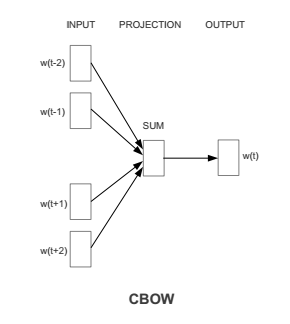
\includegraphics[width=\textwidth]{images/fig-2-cbow}
    \caption{Modelo Continuous Bag-of-words}
    \label{fig:cbow}
  \end{subfigure}
  ~
  \begin{subfigure}[b]{0.45\textwidth}
    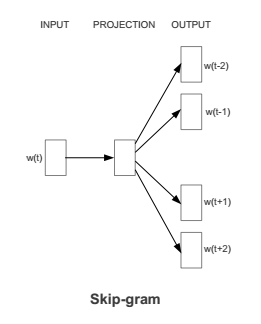
\includegraphics[width=\textwidth]{images/fig-2-sg}
    \caption{Modelo Skipgram}
    \label{fig:sg}
  \end{subfigure}

  \caption{Esquemas de word2vec}
\end{figure}

En los dos casos la probabilidad se modela utilizando exclusivamente un softmax jerárquico, como el
propuesto por Morin y Bengio en~\cite{MorinBengio2005}, con el fin de mejorar la eficiencia. Estos
dos nuevos modelos logran, por lo tanto, mejorar los resultados en la tarea de analogías a un costo
computacional significativamente menor que el de entrenar una RNN completa.

Cabe notar que, mientras que el autor lo plantea como la utilización de una red neuronal de una
única capa, también se puede ver directamente como una regresión logística multinomial, por lo que
el modelo se está simplificando enormemente con la finalidad de mejorar la eficiencia computacional,
en especial cuando se lo compara con modelos basados en RNNs. Dado el \textit{trade-off} que existe
entre la complejidad de los modelos estadísticos y la cantidad de datos que éstos pueden procesar,
este punto ubica a la propuesta de Mikolov como un modelo simple que requiere de muchos datos. De
hecho, en las pruebas que realiza el autor se utilizan corpus de texto del orden de los miles de
millones de palabras y, cuanto más aumenta el tamaño del mismo, mejores resultados obtiene.

En~\cite{Mikolov2013c}, Mikolov cierra su trabajo en representaciones vectoriales de palabras
presentando extensiones sobre el modelo Skipgram. El artículo comienza formalizando el modelo: se
presenta la función objetivo, que previamente había obviado, y se detalla la utilización del softmax
jerárquico. Luego se presenta una alternativa a esta última técnica que logra mejorar
significativamente los resultados, basada en \textit{Noise-contrastive Estimation} (NCE), propuesta
inicialmente por Gutmann y Hyyvärinen~\cite{Gutmann2012} y aplicada por Mnih y Teh para modelado de
lenguaje~\cite{MnihTeh2012}. Esta técnica, que denomina \textit{negative sampling} (NS), se basa en
generar ejemplos negativos de uso del lenguaje: esto es, además de utilizar el texto proveniente del
corpus de entrenamiento, se genera texto aleatorio, bajo la premisa de que será inválido
gramaticalmente, como ejemplo de mal uso del lenguaje.

El autor también presenta una serie de heurísticas para el procesamiento del corpus, como la
realización de \textit{subsampling} de palabras muy frecuentes (i.e.\ ignora aleatoriamente palabras que
son demasiado comunes en el corpus) y la eliminación de palabras muy raras, que mejoran aún más los
resultados.

Por último, junto a la publicación de este artículo, Mikolov presenta un nuevo conjunto de pruebas
mucho más extenso, que abarca tanto casos sintácticos como semánticos. También hace pública su
implementación de los modelos CBOW y Skipgram, bajo una herramienta denominada
\texttt{word2vec}. Este punto no es de menor importancia, porque contribuyó a aumentar el interés en
el tema, en especial entre el público amateur, y permitió reproducir y comparar los resultados con
distintos métodos de manera más correcta desde un punto de vista metodológico.


\section{Modelos Híbridos}

Los dos tipos de representaciones vectoriales descritos tienen mucha literatura detrás, pero al
haber surgido independientemente, carecían de comparaciones sistemáticas y completas entre ellos. La
primera de estas evaluaciones se realiza en~\cite{Baroni2014}.

En este artículo, los autores reúnen catorce conjuntos de pruebas utilizados por la comunidad para
los problemas de similitud entre palabras, analogías, y otros. Someten a estas pruebas a modelos
estadísticos (modelos basados en contar, como los llama el autor) y a modelos neuronales (modelos
basados en predecir). Para los primeros utiliza vectores construidos con la herramienta
\texttt{DISSECT}~\cite{Dinu2013}, basados principalmente en esquemas PMI con reducción de
dimensionalidad con SVD\@. Para los segundos utiliza la herramienta provista por Mikolov
en~\cite{Mikolov2013c}, \texttt{word2vec}.

Los resultados que obtienen los autores presentan a los modelos neuronales como grandes ganadores,
donde obtienen mejores resultados en todas las pruebas realizadas. Esta conclusión lleva a la
comunidad a investigar qué es lo que hace mejores a los métodos neuronales por sobre los
estadísticos.

Siguiendo esta línea de pensamiento, en~\cite{Levy2015} el autor busca identificar qué es lo que
hace que Skipgram con Negative Sampling (SGNS) funcione tanto mejor que un modelo PPMI que utiliza
SVD\@. Los resultados a los que llega, sin embargo, son contradictorios con los de Baroni. Plantea
que la diferencia entre la performance de ambos métodos se debe a que SGNS tiene una ventaja por
utilizar, además del modelo básico, una serie de heurísticas en el preprocesamiento del corpus y el
posprocesamiento de los vectores que mejoran drásticamente los resultados.

De esta forma, Levy identifica una serie de nueve heurísticas de uno y otro modelo, que los
considerará hiperparámetros, y los adapta para ambos esquemas. Además de hacer esto, entrena todos
los vectores utilizando exactamente el mismo corpus de datos (punto que no hizo Baroni, pues utilizó
vectores preentrenados descargados de Internet) y compara contra el mismo conjunto de pruebas. Así,
utilizando una metodología más robusta que en el estudio anterior, llega a que los resultados de los
modelos estadísticos y los modelos neuronales son prácticamente equivalentes, con los primeros con
una leve ventaja. De todos modos, el autor resalta que SGNS es mucho más eficiente
computacionalmente, lo que le permite utilizar más datos.


Más allá de las comparaciones, los dos enfoques anteriores no son necesariamente
ortogonales. En~\cite{Levy2014a} se muestra que SGNS está en realidad siguiendo un esquema muy
similar a los enfoques estadísticos, donde se realiza una factorización implícita de una matriz
SSPMI\@: esto es, una matriz PPMI donde la medida de asociación es $f(v_i, v_j) = \max(PMI(v_i, v_j)
- \log(k), 0)$, con $k$ un hiperparámetro del modelo. Este resultado es muy importante, pues conecta
directamente dos enfoques históricamente independientes. El autor plantea que la ventaja que SGNS
tiene sobre la matriz PPMI estándar se da en que su factorización está ponderada de modo de no dar
demasiada importancia a las palabras más comunes, una de las debilidades principales de la métrica
PPMI\@.


Siguiendo estos resultados, han surgido diversos métodos que plantean un esquema híbrido, donde se
busca hacer explícita la tarea de aprendizaje que se realiza, basándose en las lecciones aprendidas
de los enfoques ya presentados. Uno de estos métodos es GloVe, presentado en~\cite{Pennington2014},
donde los autores construyen una matriz $A$, similar a la matriz de asociación de los modelos
estadísticos, donde la función de asociación busca explícitamente quitar peso a las palabras más
frecuentes y no sobrerrepresentar a las muy poco frecuentes. Luego obtiene representaciones
vectoriales de baja dimensionalidad minimizando una función de costo asociada los vectores de
palabras y la matriz de coocurrencia, siguiendo un método iterativo que lo hace computacionalmente
más eficiente que SVD\@. Los resultados que obtienen los autores son superiores a los obtenidos por
SGNS en el conjunto de pruebas provisto por Mikolov\footnote{Cabe notar que en~\cite{Levy2015} no se
logra reproducir este resultado, aunque aun así es un método muy competitivo.}.


Los modelos estadísticos, neuronales e híbridos han resultado bastante similares en cuanto a los
resultados obtenidos. Reconociendo este punto, la comunidad se está centrando en modelos híbridos
que aprovechen las lecciones aprendidas por los tres enfoques, buscando nuevas métricas de
asociación (definiendo matrices de asociación explícitamente) y nuevas formas de factorizarlas (ya
sea con variantes de SVD, o con métodos iterativos).


\section{Evaluación y Estado del Arte}

Hasta ahora se presentaron distintos enfoques para la construcción de representaciones vectoriales,
pero no se ha detallado qué entendemos por estado del arte: esto es, cuándo consideramos que una
representación es mejor que otra, y cómo las comparamos.

Es posible comparar las representaciones de forma implícita y explícita. La primera implica evaluar
los cambios en la performance en un algoritmo de aprendizaje automático donde se usan; esto es, como
parte de una solución de un problema de PLN más grande. La segunda refiere a evaluar directamente la
calidad de los vectores obtenidos mediante alguna tarea de PLN desarrollada específicamente para el
caso.

Para la evaluación explícita, el objetivo es diseñar un experimento cuyo resultado esté, en la
medida de lo posible, correlacionado a la calidad de una solución de PLN de mayor porte cuando se
utilizan estas representaciones. Esto permite optimizar una métrica más definida y más fácil de
calcular. Por ejemplo, si se está construyendo una solución para el procesamiento automático del
habla (ASR), y se supiera que representaciones que funcionan mejor en la tarea de analogías mejoran
el resultado final, sería mucho más fácil y eficiente probar distintos hiperparámetros y modelos
evaluando con esa métrica, que entrenar todo un modelo de ASR de principio a fin para evaluar si los
vectores produjeron mejores resultados\footnote{Esto es particularmente problemático para los
vectores de palabras, pues suelen ser el primer componente en una solución PLN.}. En especial porque
en un modelo complejo, pueden haber varios componentes que afecten la calidad final de la solución,
por lo que no se sabrá si fueron los vectores los que mejoraron los resultados o no.

De todos modos, esta correlación entre la evaluación explícita e implícita de representaciones
vectoriales por lo general no se puede probar, y es una suposición que se toma cuando se realiza una
evaluación explícita.


En la literatura se han usado muchas tareas para la evaluación explícita de vectores, algunas de las
cuales ya han sido mencionadas brevemente. Una de las más antiguas es la tarea de similitud y
relación entre palabras, que busca decidir si una palabra es sustituible por otra en un contexto
dado. Para esto, se construye un conjunto de pruebas compuesto por pares de palabras y un puntaje,
determinado por un grupo de humanos, de qué tan similares son dichas palabras. El objetivo es
obtener un buen nivel de correlación entre los puntajes de los pares de palabras y las
distancias\footnote{Es usual utilizar la distancia euclídea o la distancia coseno.} en el espacio de
vectores, medida utilizando la correlación de Spearman. Distinguimos también entre similitud, donde
se mide relaciones más fuertes, como la sinonimia y la hiponimia, de la relación
(\textit{relatedness} en la literatura), donde se incluyen relaciones más amplias, posiblemente
temáticas.

Existen muchos conjuntos de prueba para esta tarea. Uno de los más utilizados es
WordSim353~\cite{Finkelstein2002}, compuesta de 353 pares de palabras, diferenciados entre relación
y similitud. También muy populares están MEN~\cite{Bruni2012}, compuesto de 1000 pares de palabras,
SimLex999~\cite{Hill2014}, y Mechanical Turk~\cite{Radinsky2011}.

Otra alternativa que ha surgido recientemente para el estudio de regularidades lingüísticas de
representaciones vectoriales es la tarea de analogías, propuesta inicialmente por Mikolov
en~\cite{Mikolov2013a}. En este escenario, se cuenta con dos pares de palabras que mantienen una
misma relación (sintáctica o semántica) y se busca determinar la cuarta palabra a partir de las
anteriores tres. Por ejemplo, si se cuenta con los pares de palabras \textit{correr} y
\textit{corriendo}, \textit{jugar} y \textit{jugando}, el objetivo es, a partir de los vectores de
\textit{correr}, \textit{corriendo} y \textit{jugar}, lograr recuperar la cuarta palabra,
\textit{jugando}.

Para esto Mikolov originalmente propone en~\cite{Mikolov2013a} utilizar la función \textsc{3CosAdd}
para recuperar la cuarta palabra, definida como:

\[
  {\arg \max}_{b' \in V} \cos(b', b - a + a')
\]

Donde los pares de analogías son $(a, a')$ y $(b, b')$ y $\cos$ la similitud coseno. Sin embargo,
en~\cite{Levy2014b}, Levy prueba que una mejor función para la recuperación de analogías es
\textsc{3CosMul}, definida como:

\[
  {\arg \max}_{b' \in V} \frac{\cos(b', b) \cos(b', a')}{\cos(b', a) + \epsilon}
\]

Donde $\epsilon$ es un valor muy pequeño (e.g.\ $\epsilon = 0.001$) utilizado para evitar la
división entre cero.

Mikolov introdujo inicialmente un conjunto de 8000 analogías exclusivamente sintácticas
en~\cite{Mikolov2013a}, con relaciones como plurales y conjugaciones verbales. Luego introduce
en~\cite{Mikolov2013b} un conjunto de analogías más amplio que cuenta con cerca de 20000 analogías,
tanto sintácticas como semánticas.

Existen también otras tareas que se han utilizado, aunque en menor medida, para la evaluación
explícita de vectores, como la utilización del TOEFL (\textit{Test of English as Foreign Language},
una prueba utilizada para medir el conocimiento de inglés) de~\cite{LandauerDumais1997}, la
categorización de conceptos de~\cite{Almuhareb2006}, y la preferencia de selección
de~\cite{Pado2007}.


En cuanto a evaluación implícita de las representaciones vectoriales, y cómo se relaciona con los
resultados de la evaluación explícita, no existe mucho trabajo en la literatura. Un trabajo
preliminar que toca superficialmente este punto es~\cite{Qu2015}, donde los autores utilizan
distintos modelos vectoriales (SGNS, GloVe, los vectores de Collobert y Weston, y Brown Clusters)
como features de algoritmos de clasificación secuencial (principalmente CRFs, para resolver los
problemas de POS tagging y NER). Llegan a que, al usar distintas representaciones bajo este esquema
(donde los vectores son una feature más), los resultados mejoran de manera muy similar para los
distintos modelos: esto es, se obtiene la misma ganancia utilizando Brown Clusters (que genera una
representación más rudimentaria) que SGNS\@.

Existe también un poco de escepticismo por parte de algunos investigadores en el área respecto a qué
beneficios proveen los vectores de palabras. Edward Grefenstette escribe~\cite{Reddit2016} que las
representaciones vectoriales parecen ser principalmente una forma de aprendizaje por transferencia,
donde se entrena con la tarea de analogías o similitud entre palabras para resolver una tarea más
compleja. Plantea que esto es beneficioso cuando se trabaja con corpus de entrenamiento demasiado
chicos, pues ayuda a la generalización, pero que no son necesarios e incluso pueden perjudicar la
performance cuando se tienen suficientes datos.

Otro caso que fortalece este argumento es el hecho que en~\cite{CollobertWeston2008} se obtienen muy
buenos resultados en el etiquetado de roles semánticos, pero los vectores son inferiores en la tarea
de analogías (como muestra~\cite{Mikolov2013a}). Esto, de todos modos, puede resultar del hecho que
los autores ajustan los valores de los vectores en la medida que entrenan con las otras tareas.

Estos puntos son importantes y requieren de mayor investigación, pues determinan qué tanto es
necesario buscar nuevos y mejores modelos vectoriales. Es posible, por ejemplo, que pequeñas
diferencias en los resultados de evaluación explícita sean compensados por el modelo que los usa,
como pasa con los Brown Clusters en~\cite{Qu2015}. En este caso, se podría incluso utilizar un
corpus más chico para entrenar las representaciones, o vectores más simples.


De todos modos, en el presente proyecto se estará realizando una evaluación puramente explícita de
los modelos vectoriales entrenados, por varias razones. En primer lugar, el objetivo es realizar una
investigación del comportamiento de representaciones vectoriales en general, no de un problema de
PLN particular. Segundo, porque no hay un estándar en evaluación implícita con el que se pueda
comparar los resultados, ni que sean una aplicación directa de vectores de palabras. Tercero, porque
realizar una evaluación implícita sería mucho más costoso computacional y metodológicamente, lo que
nos impediría probar con una gran variedad de modelos. Y por último, porque las tareas con las que
se estarán evaluando, analogías y similitud de palabras, entre otros, tienen de por sí aplicaciones
directas que son de gran utilidad.


En cuanto a los modelos vectoriales que se evaluarán, se decidió optar por un representante de cada
enfoque: Skipgram y CBOW como modelos neuronales, una matriz PPMI con SVD como modelo estadístico, y
GloVe como modelo híbrido. Se eligen estos cuatro modelos por ser los que consiguen los mejores
resultados en las tareas de analogías y similitud de palabras en la literatura en inglés, evitando
así sesgarnos a un esquema de representación vectorial particular, y pudiendo evaluar si alguno de
ellos tiene un comportamiento particular para el idioma español.

\chapter{Corpus}

El tamaño del corpus de texto utilizado para entrenar las representaciones vectoriales está
fuertemente ligado a la performance que éstas consiguen en las principales tareas de evaluación,
como se detalló en el capítulo anterior. Esto genera la necesidad de construir un corpus de texto en
idioma español del mayor tamaño posible, buscando que sea comparable con los que se manejan en la
literatura en inglés.

El capítulo empieza por presentar el relevamiento realizado sobre el tamaño y calidad de los corpus
en español existentes. Luego se plantean los requerimientos y características que se consideró que
el corpus debía contener, y se da una visión general del proceso empleado para lograrlo. Finalmente,
se detalla la implementación de dicho esquema y se resumen las características del coprus
construido.

\section{Estado del Arte}

Como ya se mencionó, una de las claves principales para la calidad de los vectores generados es contar
con un corpus de gran tamaño, compuesto de documentos con estilos de redacción y temáticas variadas.
Se procedió por tanto a investigar la oferta existente de corpus en idioma español en internet. En esta
sección se discutirán los proyectos de construcción de corpus más relevantes, detallando de cada uno su
composición, medidas de calidad y limitantes de acceso ó uso, en caso de haberlas.

La investigación incluida en esta sección no pretende ser completamente exhaustiva, pero si lo
suficientemente profunda como para justificar la decisión de construir un nuevo corpus en el presente
proyecto en lugar de utilizar alguno ya existente para el entrenamiento de vectores. Como se verá, muchos
de los proyectos de construcción de corpus existentes no cumplen con las condiciones más importantes
requeridas por el presente proyecto.

Se procedió entonces a realizar una investigación formal de las alternativas existentes. Una de las
fuentes consultadas fue la investigación realizada en el año 2009 por el Centro Virtual Cervantes [CITA3].
En su trabajo los autores dan cuenta de la existencia de diversos proyectos para la construcción de corpus
en español clasificándolos en distintas categorías, entre ellas el tamaño de los corpus construidos y la
capacidad de acceso a los textos que forman los mismos. Estás características son, naturalmente, muy
relevantes para la tarea de construcción de vectores de palabras. A pesar de su considerable valor, la
investigación realizada por los autores apunta a corpus de muy diversos tipos, incluyendo grabaciones
de entrevistas orales, y no resultó ser una referencia definitiva para nuestra investigación.

Aún así, la investigación del Instituto Virtual Cervantes resultó un buen punto de partida para nuestro
relevamiento. Resulta interesante destacar que los autores obtienen entre sus principales conclusiones
que la mayoría de los trabajos analizados contaron, en alguna medida, con apoyo económico de entidades
privadas o gubernamentales para su desarrollo. Consideramos que este hecho pone en perspectiva los logros
obtenidos en el presente proyecto de grado para la construcción de un corpus masivo, cuyos detalles se
explicarán en las secciones posteriores.

\subsubsection{Wikipedia}

Como punto inicial es interesante considerar el corpus formado por todos los artículos de Wikipedia.
La enrome cantidad de artículos abarcando una multitud de temáticas junto con su esencia libre y abierta
hacen de Wikipedia una elección natural para tareas de PLN que requieren una gran cantidad de texto
[CITA1]. En idioma inglés, Wikipedia contiene casi tres billones de palabras repartidas en aproximadamente
cinco millones de artículos [Cita2]. En idioma español la cifra es mucho menor, ubicándose en 400 millones
de palabras. Por tanto, quedó claro desde un principio que utilizar un corpus constituido únicamente
por artículos de Wikipedia no sería suficiente.

\subsubsection{Sketch Engine: TenTen}

Se consideró también el trabajo realizado por la organización Sketch Engine [cita], organización
dedicada a la construcción de corpus masivos en varios idiomas y la elaboración de herramientas
para la manipulación y consulta de los corpus generados, pensadas para profesionales de distintas
áreas. Entre los corpus ofrecidos por Sketch Engine se destaca principalmente el proyecto TenTen [cita].
TenTen consiste en una colección de corpus repartidos en varios idiomas superando en varios de ellos la
barrera del billón de palabras. Para el caso concreto del español se tiene un corpus de ocho billones de
palabras. El corpus TenTen es catalogado por sus autores como un corpus web, lo que implica que para
su construcción se utilizaron únicamente textos disponibles en Internet.

Existen diferentes estrategias para la construcción de corpus basados en Internet. En el caso de TenTen
los autores utilizaron un proceso basado en crawling masivo, limpieza de documentos, detección de
duplicados y almacenamiento. Para esto los autores construyeron varias herramientas que posteriormente
liberaron como código abierto.

Para la tarea de crawling masivo en la construcción de TenTen se usó la herramienta Spiderling [CITA4],
desarrollada especialmente para la construcción de corpus utilizando Internet. En la experiencia de los
autores, el principal problema de los corpus web es la enorme cantidad de páginas que es necesario
descargar para obtener una cantidad relativamente pequeña de texto útil. En su análisis definen la
medida \textit{tasa de rendimiento} (\textit{yield rate}), que se aplica a cada página web descargada y
expresa la relación entre la cantidad de bytes de la página y la cantidad de bytes de información útil
obtenida a partir de la misma:

\[
  \textit{tasa de rendimiento} = \frac{\textit{tamaño de datos útiles obtenidos}}{\textit{tamaño total de la página}}
\]

Spiderling buscará de esta manera priorizar dominios que presenten tasas de rendimiento altas en el
conjunto de sus páginas, permitiendo una extracción inicial a modo de muestra para decidir luego si
vale la pena continuar procesando el dominio o si es mejor descartarlo. De este modo los autores aseguran
que se obtiene un ahorro importante de ancho de banda y de tiempo de limpieza sin apenas comprometer
el tamaño final que tendrá el corpus generado.

Naturalmente, luego del proceso de crawling es necesario extraer el texto útil a partir del código
HTML descargado. En el caso de TenTen, los autores utilizaron herramientas construidas por ellos mismos
para eliminar etiquetas HTML y texto \textit{boilerplate} [CITA5]. La definición de este último concepto
es difícil y suele depender del contexto de su aplicación. En nuestro caso consideramos como
\textit{boilerplate} aquel texto que refiere a la estructura y navegación de una página web y no a su
contenido real. Por ejemplo, texto de enlaces de una barra de navegación, texto perteneciente a secciones
de publicidad, metadatos de la estructura del sitio, etcétera.

Lamentablemente, los corpus generados por Sketch Engine no están disponibles de forma gratuita. La
organización ofrece en su sitio web un período de prueba sin costo para acceder a los mismos, pero la
utilización prolongada de sus servicios requiere una subscripción. Esta modalidad de uso, además de estar
por fuera del alcance de este proyecto de grado, entra en conflicto con uno de nuestros principales
objetivos, como es la publicación total del corpus construido para el entrenamiento de vectores de palabras.

\subsubsection{Linguistic Data Consortium: Gigaword en español}

Otro corpus que vale la pena analizar es el corpus Gigaword en español construido por el Linguistic Data
Consortium (LDC) [CITA]. El LDC es un consorcio de universidades, bibliotecas y laboratorios de
investigación gubernamentales creado para enfrentar el problema de escasez de datos en las áreas de
investigación vinculadas al lenguaje.

El corpus Gigaword, en su tercera edición, cuenta con más de un billón da palabras repartidas en casi
cuatro millones de documentos almacenados en formato SGML/XML [CITA6]. Los documentos utilizados para
construir el corpus son en su totalidad cables de noticias provistos por las agencias internacionales
Agence France-Presse, Associated Press (AP) y Xinhua News Agency.

Los documentos del corpus fueron catalogados por los autores, aunque estos advierten que las categorías
asignadas son simplemente aproximaciones. Dichas categorías no son de mucha utilidad pues apenas
distinguen entre reportes, aquellos que pueden encontrarse en cualquier revista de noticias, y cables
dirigidos a editores y reporteros de periódicos. En cuanto a la calidad, los autores sólo aseguran
controles exhaustivos en el formato de los datos, eliminado errores de recepción que corrompan el
texto original. Se realiza también un proceso de filtro de cables repetidos, aunque se menciona que
dicho proceso no es totalmente riguroso. Los autores advierten que es probable encontrar algunos
errores de redacción o de ortografía, típicos del ritmo y exigencias diarias que se dan en los
periódicos y agencias de noticias.

Como ocurre con TenTen el acceso a Gigaword no es gratuito, salvo para miembros del LDC. Los costos de
adquisición del corpus resultan prohibitivos para el alcance de el presente proyecto y, como ya se
mencionó, esta modalidad de distribución tampoco se alinea con los objetivos del proyecto.

\subsubsection{Universidad de Brigham Young: Corpus del Español}

El Corpus del Español es un proyecto elaborado por Mark Davies del departamento de lingüística de
la Universidad de Brigham Young y financiado a través de una subvención del fondo nacional
estadounidense \textit{US National Endowment for the Humanities} [CITA7]. Este corpus está compuesto
por cien millones de palabras, la cual es una cantidad relativamente pequeña si la comparamos con las
cantidades de los proyectos ya analizados. Sin embargo,  este corpus cuenta con la particularidad de
contener documentos de bastante antigüedad, abarcando el período desde el siglo XIII al siglo XX.
Recientemente, el proyecto recibió una beca para extender el tamaño del corpus a dos billones de
palabras. Dicha extensión comenzó a realizarse en 2015 y continuará durante el año 2016.

En la descripción de su trabajo, Davies explica los motivos para construir este corpus en español
habiendo ya alternativas disponibles de mucho mayor tamaño. Su argumento principal es que el tamaño
no lo es todo y resulta muy importante contar con un corpus correctamente anotado y etiquetado para
que este pueda ser de utilidad en la mayoría de las tareas. En su crítica a otros proyectos el autor
argumenta que en la mayoría de los casos se aprecia un bajo conocimiento del idioma español por parte
de los encargados de los mismos y que el etiquetado de los corpus publicados fue hecho de manera
automática sin prestar demasiada atención al resultado final.

Curiosamente, y a pesar de que los argumentos de Davies no deben ser despreciados, en el caso del
entrenamiento de vectores de palabras con los algoritmos que nos competen en este trabajo, no es
necesario contar con un corpus anotado y etiquetado, como lo es en una gran cantidad de aplicaciones.

Finalmente, el acceso al Corpus del Español es totalmente gratuito, aunque no cuenta con mecanismos
explícitos para descargarlo en su totalidad. Además, y de forma entendible, las consultas al corpus
están limitadas de forma diaria por usuario registrado y por dirección IP para usuarios anónimos.
Estas limitantes de acceso, sumadas a las características ya descritas, hacen que este corpus no sea
de gran utilidad para el presente proyecto.

\subsubsection{Corpora from the Web: ESCOW14}

El proyecto Corpora from the Web (COW) es una iniciativa del grupo de gramática y lingüísticas
generales de la Universidad Libre de Berlín (Freie Universität Berlin) [CITA]. El proyecto consta
de una colección de corpus web en varios idiomas, entre los que se encuentra el español. Para este
caso se cuenta con ESCOW14, un corpus en español de más de siete billones de palabras repartidas en
cinco millones de documentos. El corpus fue generado realizando crawling masivo en Internet y en su
versión actual cuenta con documentos del período comprendido entre 2012 y 2014, abarcando además
documentos de una gran cantidad de países.

Para la limpieza de documentos obtenidos de la web y posterior extracción de texto útil se utilizó
texrex, una herramienta creada por Roland Schäfer, integrante del equipo de COW. La herramienta cuenta
con funcionalidades para filtrar duplicados, remover código HTML, extraer metadatos de los cabezales
HTTP obtenidos del proceso de crawling, normalización de codificación de caracteres a UTF-8, entre
otras. Este proceso resulta de mucha importancia, pues en su descripción del corpus los autores
mencionan que una de sus grandes prioridades es generar corpus de alta calidad y no solamente
conformarse con construir corpus con grandes cantidades de palabras.

El acceso a ESCOW14 está altamente limitado por los autores y regido por políticas de acceso muy
estrictas, en un esfuerzo por ajustarse a las leyes alemanas de derecho de autor. Por este motivo
los autores sólo ofrecen para descargar grupos de oraciones mezcladas lejos de su contexto original
y no permiten acceso directo a los documentos originales. Además, para obtener acceso a este contenido
es necesario completar un formulario detallando el uso que se planea hacer del corpus, entre otros
datos. Lamentablemente, al momento de escribir este informe aún no fuimos capaces de obtener acceso
a ESCOW14.

\subsubsection{Conclusiones}

---- Conclusiones acá ----
TODO: - Arreglar formato, corregir, agregar citas y escribir conclusiones.
--------------------------

\section{Proceso de Construcción}

En esta sección se presentan las características buscadas del corpus a generar y el proceso seguido
para lograrlo.

\subsection{Requerimientos}

Previo al inicio de la construcción del corpus, se establecieron una serie de requerimientos que el
mismo debiera cumplir:

\begin{itemize}

\item Puesto que el tamaño del corpus afecta directamente la calidad de las representaciones
vectoriales, es claro que el principal requerimiento es que el resultado tenga una gran cantidad de
palabras. El mínimo que se planteó al inicio del proyecto fue de dos mil millones de palabras (para
comparar, el corpus en inglés utilizado por Mikolov en~\cite{Mikolov2013c} ronda los seis mil
millones de palabras).

\item La única restricción que se plantea sobre el contenido es que sea texto en forma libre (sin
ningún tipo de estructura a priori), y que esté limpio: esto es, que no cuente con \textit{markup}
de ningún tipo. Dado que los algoritmos para construir los vectores trabajan con una secuencia de
palabras sin formato alguno, es deseable que el texto se procese incluso antes de ser almacenado,
para evitar tener que tratarlo más adelante.

\item Se desea que el corpus esté dividido en documentos individuales que sean coherentes en sí
mismo, manteniendo un determinado estilo de escritura internamente. Así, artículos de noticias serán
almacenados individualmente, y lo mismo con libros, artículos de Wikipedia, y cualquier otro texto
que se recopile. El objetivo de este punto es permitir excluir o borrar un documento particular en
caso de ser necesario.

\item Se espera también que estos documentos puedan tener ciertos metadatos asociados. Algunos de
estos datos pueden aplicar a todos los documentos, como la fecha en la que fue agregado al corpus,
mientras que otros sólo tendrán sentido para un subconjunto, como la fecha de publicación de una
noticia. Esto puede permitir eventualmente construir un corpus con las noticias de un año
particular, para poder generar representaciones vectoriales más finas.

\item Es de suma importancia tener trazabilidad sobre los distintos documentos del corpus para
garantizar su calidad: esto es, saber de qué sitio se extrajo el texto de cada documento, en qué
fecha, y mediante qué proceso. Así, en caso de haber un problema en el proceso de extracción, es
siempre posible revertir el corpus a un estado anterior, eliminando todos los documentos
erróneos. Este punto permite además evitar almacenar más de una vez un documento particular, y ayuda
también a identificar cuáles contenidos están protegidos por \textit{copyright}.

\item Con el fin de generar buenas representaciones vectoriales, es importante que el corpus cuente
con variedad de texto: texto que tenga distintos estilos de escritura, que utilicen vocabularios
distintos, y que tengan distintos niveles de correctitud ortográfica. Esto dota a los algoritmos de
un mayor vocabulario y de información más rica acerca del contexto en el que las palabras pueden
aparecer.

\item Por último, puesto que el corpus debe contar con gran variedad, es necesario que esté
ordenado. Se espera que cada documento esté etiquetado en base a sus cualidades, identificando
cuáles son artículos de noticias, cuáles son de determinado país, etc. Etiquetar el texto brinda la
posibilidad de construir un corpus a medida, para poder eventualmente hacer pruebas específicas que
incluyan o exculyan cierto tipo de texto.

\end{itemize}

Los requerimientos recién planteados son exigentes, pero permiten la construcción de un corpus
altamente versátil. Además de poder entrenar modelos vectoriales particulares a una aplicación (en
base al texto que se incluya en el corpus), permite que el mismo pueda ser utilizado en otras
investigaciones que no estén relacionadas a las representaciones vectoriales, pero que necesiten de
texto en español con ciertas cualidades. Mediante la inclusión de metadatos particulares, de
etiquetado según el estilo del texto, y de datos de trazabilidad para cada documento, se busca
reforzar esta idea.

El hecho de exigir tantos requerimientos, sin embargo, hace que sea necesario descartar algunos de
los corpus existentes anteriormente mencionados. [o no? Cuáles de los corpus existentes nos sirven y
cuáles no (si están limpios, clasificados, etc.)?]


\subsection{Relevamiento de Fuentes de Palabras}

Se comenzó por la tarea de evaluar de dónde obtener texto libre de Internet, con el fin de construir
un corpus de calidad que cumpla con los requerimientos anteriores. En esta sección enumeraremos los
distintos tipos de sitios de donde se recopiló el texto, junto a las características del mismo y una
breve descripción de cómo se realizó la extracción. En la siguiente sección se entrará en la
implementación de estas técnicas en más detalle.

[- comentar el tipo de texto que se saca de cada fuente]
[- comentar cómo se saca el texto limpio para cada fuente comentada]
[el objetivo de esta sección es mostrar que buscamos *muchas* fuentes de datos y nos quedamos con lo
mejor; que cada una de las fuentes cumplió con los requerimientos y más o menos qué enfoque se
utilizó para scrapearla]

[- comentar que se optó por sacar algo de cada tipo de fuentes, que en principio hay más info en cada área pero escapaba del alcance]


\subsubsection{Portales de Noticias}

La primer fuente de palabras investigada fueron los portales de noticias en línea, pues presentan
varias ventajas:\begin{inparaenum}[(a)]
\item están compuestos de texto por lo general bien escrito;
\item están divididos en documentos que tratan cada uno de un tema particular;
\item cada portal tiene un gran número de artículos y hay una gran cantidad de portales por país;
\item permiten obtener muestras de texto por país, mejorando la riqueza del corpus final; y
\item el texto es fácil de limpiar, pues el único markup con el que cuentan suele ser HTML\@.
\end{inparaenum}

En cuanto al vocabulario utilizado en los artículos de noticias, se puede considerar simple, pero
con una fuerte presencia de nombres de personas y lugares, que a su vez son dependientes de la fecha
de publicación del artículo: esto es, distintas personas tendrán más o menos menciones en períodos
particulares de tiempo. Este punto es importante, y es una de las principales razones para decidir
guardar esta fecha de como metadato del artículo.


La investigación de portales de noticias comenzó por el diario La Nación de Argentina [cita?], por
ser uno de los primeros diarios grandes en tener presencia digital, desde el año 2000. Realizando
algunos cálculos preliminares en base a un muestreo de artículos, se vio que el diario contaba con
al menos un millón de artículos, cada uno con un promedio de 500 palabras, llegando a un a masa total
de palabras muy importante.

Uno de los primeros puntos que se notó es que la URL de todos los artículos del portal estaban
identificadas por un número, y que cambiando este número por uno distinto, se podía acceder a otra
noticia. Además, la generación de estos números es secuencia: esto es, el primer artículo publicado
tiene el identificador $1$, mientras que el último el $1871018$. Este hallazgo fue de suma
importancia, pues permitió realizar \textit{scraping} del portal de forma más directa.

Aprovechando esta característica, se construyó un script en Python [cita?] para recorrer la lista de
identificadores (desde el $1$ hasta el último presente en la portada) y descargar el contenido de
los artículos. Puesto que el corpus a construir requiere de texto limpio, se generaronn una serie de
reglas XPath [cita?] para obtener los datos estructurados (título de la noticia, contenido, fecha de
publicación). Corriendo este script en la totalidad de La Nación, se llegó a la cifra de 600
millones de palabras exclusivamente con sus artículos.

Los resultados obtenidos demostraron el alto potencial que tienen los portales de noticias como
fuentes de palabras, por lo que se procedió a recopilar una lista de los principales diarios de
América Latina y España. Con el objetivo de seguir el esquema anterior, se identificaron cuáles de
estos sitios identificaban sus artículos con las mismas características, y se adaptó el anterior
script a los 20 que presentaban un mayor potencial (en base a la actividad y al contenido).

Para cada uno de estos portales, se construyeron una serie de reglas XPath para extraer el contenido
y un mecanismo para recorrer por el identificador numérico. Además se adaptó el script para que
revise de forma continua por noticias nuevas, con el fin de que el corpus se mantenga siempre
actualizado\footnote{Para ilustrar la importancia de este punto, sólo por mantener actualizado el
corpus se consiguieron 300 millones de palabras adicionales en el tiempo de proyecto
transcurrido.}. Este método lo denominamos \textit{scraping automático}, y más adelante se detallará
su implementación (por ejemplo, cómo sabe extraer los datos, cómo se define un nuevo sitio, y cómo se
hace la recorrida por identificador).

En base a esta técnica se consiguieron más de 3 mil millones de palabras de texto limpio a partir de
20 portales de noticias.


Cabe resaltar que el método anterior depende de que los artículos de noticias tengan asociado un
identificador secuencial. Lamentablemente, esto no es el caso con muchos sitios de noticias
importantes y de gran tamaño, como El País de Madrid, El País de Uruguay, o Clarín de Argentina. Por
esta razón, se decidió también emplear un mecanismo de scraping estándar mediante la herramienta
Scrapy [cita?] para estos portales, implementación que se detalla más adelante.


\subsubsection{Escritura Amateur}

Existen diversos sitios en Internet dedicados a la escritura amateur, donde los usuarios se
registran y publican historias propias. Puesto que muchos de estos sitios acumulan una gran cantidad
de historias, se decidió investigar esta área en mayor profundidad.

Algunos de estos sitios, como Los Cuentos [cita], son de carácter más bien general, donde los
usuarios publican narraciones, ensayos, cuentos o poemas. La calidad y el contenido de estos textos
varía drásticamente entre uno y otro, pudiendo encontrar piezas con una gran cantidad de faltas de
ortografía y carentes de sentido, o piezas por autores renombrados que fueron republicados en el
sitio.

La otra gran categoría de escritura amateur presente en Internet es el \textit{fanfiction}
(\textit{ficción de fans}, en inglés). Estos textos suelen ser escritos principalmente por jóvenes,
centrados en universos o personajes de la cultura popular, como series de televisión, videojuegos o
libros. Debido a esto, su calidad suele ser incluso inferior al anterior grupo. Suelen contener
grandes cantidades de diálogo (como si fuera un guión) y muchas menciones a personajes o lugares
ficticios.

De todos modos, la media de los textos obtenidos de estas fuentes de palabras está compuesta por
oraciones coherentes y con relativamente pocas faltas de ortografía, por lo que es de gran utilidad
para el corpus que se pretende construir. Además, existe un gran volumen de datos, y el texto es
fácil de limpiar.

Para atacar estos sitios, se optó por usar principalmente la técnica de scraping automático
mencionada en la sección anterior, pudiendo así incorporar al corpus nuevas historias en la medida
que se escriban.


\subsubsection{Wikimedia}

Los distintos proyectos de Wikimedia [cita], como Wikipedia, Wikilibros, Wikicitas, y Wikiviajes,
son una fuente de palabras particularmente interesante, pues tiene todas las cualidades que se
espera del corpus:

\begin{itemize}

\item En primer lugar, cuentan con grandes volúmenes de texto que ayudan a llegar a la meta
propuesta. El principal proyecto de Wikimedia es Wikipedia, pero el resto tienen cantidades no
despreciables de palabras también.

\item Segundo, tienen una gran variedad de contenidos, en especial Wikipedia: siendo una
enciclopedia, posee entradas y menciones para países, personas, lugares, eventos, fenómenos, etc.,
dotando así al corpus de un gran y diverso vocabulario, lo cuál será muy positivo al entrenar
modelos vectoriales.

\item Tercero, el texto está bien escrito y suele ser activamente revisado por distintas personas,
por lo que el nivel de calidad es superior al resto de las fuentes.

\item Cuarto, se encuentra dividido en artículos bien delimitados que tratan de un único tema
particular, permitiendo obtener resultados más coherentes cuando se realizan búsquedas sobre el
corpus.

\end{itemize}


El contenido de los proyectos de Wikimedia puede ser descargado en línea a través de \textit{dumps}
provistos por la fundación misma [cita]. La principal complejidad de incorporar esta fuente es, sin
embargo, su limpieza, pues los artículos vienen con un \textit{markup} denominado \textit{wikitexto}
[cita] que dificulta la extracción del texto. De todos modos, existen una gran variedad de
herramientas para la limpieza del mismo, cuestión que se detallará más adelante.


\subsubsection{Foros}

Los foros de discusión de Internet [cita] son otra gran fuente de palabras, en cuanto al volumen de
datos. Dado que muchos poseen miles de usuarios registrados, llegan a manejar cantidades de texto
muy elevadas. Como contrapartida, sin embargo, el texto publicado suele ser de muy baja calidad,
donde algunos mensajes no son más que imágenes o emotíconos y por lo tanto carentes de contenido
útil para el propósito del proyecto. Esto último depende también de la audiencia que interactúe en
dicho foro, donde sitios con una demografía de edad mayor suelen tener mejor calidad.

De todos modos, se decidió utilizar estas plataformas como fuentes de noticias porque permiten
experimentar con la calidad de los modelos vectoriales en función a la calidad del corpus. Además,
puesto que suelen tener un estilo más similar al habla, tienen vocabularios distintos al resto de
las fuentes y consecuentemente una mayor cantidad de expresiones del argot de los participantes.

Se utilizaron técnicas de scraping a través de Scrapy para extraer el contenido de estas fuentes,
punto que se detallará en la sección siguiente.


\subsubsection{Subtítulos}

Hay una gran cantidad de texto en los subtítulos de series y películas extranjeras. Como referencia,
los subtítulos de un capítulo de una serie de televisión de una hora rondan las cinco mil
palabras. Dada la enorme cantidad de series existentes, cada una con decenas de episodios, se llega
a un volumen de palabras muy alto.

El texto de los subtítulos por lo general está correctamente escrito, aunque se compone casi
exclusivamente de diálogos. Esto también provee otro tipo de vocabulario distinto a las fuentes
anteriores pues, por ejemplo, hay un mayor uso de la segunda persona.

La descarga de los subtítulos se realizó con un script manual, bajando todo el contenido disponible
en Tu Subtítulo [cita]. Luego fue necesario extraer el texto de los mismos, eliminando las
indicaciones de tiempo (cuándo debe aparecer cada línea en pantalla) y el markup que pueden contener
(tags HTML por lo general).


\subsubsection{Documentos Oficiales}

Muchas instituciones públicas publican grandes cantidades de textos con el fin de informar a sus
poblaciones sobre distintos temas, o de mantener registro de las actividades de sus
representantes. Entre este tipo de texto se encuentran las versiones taquigráficas de sesiones de
parlamentos de países u organizaciones internacionales, como la UE o UNASUR, así como comunicados de
distintas instituciones como la ONU\@. Estos textos suelen tener una jerga partícular, pues son
muchas veces documentos altamente técnicos, pero son no obstante textos de calidad que pueden
aportar mayor volumen y vocabulario al corpus.

Se incorporaron dos fuentes de documentos oficiales al corpus: los diarios de sesiones del
parlamento Uruguayo del año 1985 a la fecha y los comunicados emitidos por la ONU entre los años
1999 a 2009.

El primero fue descargado a través de un script de la página del Poder Legislativo Uruguayo [cita] y
luego procesado para eliminar el markup. Contiene las sesiones de la Cámara de Diputados, la Cámara
de Senadores, y de la Asamblea General. El mecanismo para su descarga se detalla más adelante.

El segundo fue tomado de un corpus paralelo generado por [cita] como insumo para tareas de
traducción automática. Fue descargado de [cita http://opus.lingfil.uu.se/MultiUN.php], procesado y
finalmente agregado al corpus construido.


\subsubsection{Libros}

Una fuente de palabras inmediata son libros de texto en español, pues se cuenta con cientos de
miles, cada uno de gran tamaño. En la mayoría de los casos también son revisados por un editor, por
lo que la calidad de la escritura es superior a la encontrada en las otras fuentes. Además cuentan
con una gran variedad de vocabulario, pues su contenido va desde de ficciones narrativas hasta
textos científicos.

La incorporación de libros en el corpus presenta, sin embargo, varias dificultad: en primer lugar,
no es fácil acceder digitalmente a colecciones importantes de libros, pues no están disponibles de
manera pública en Internet fácilmente. Segundo, incluso cuando sí es posible obtener libros
digitalmente, suelen estar en formatos que hacen la extracción de texto muy compleja (por ejemplo,
PDFs con escaneos del texto).

Se optó por utilizar un corpus ya existente que recopila textos relacionados a la Unión Europea (en
particular a su librería, \textit{EU Bookshop} [cita]), provista por el proyecto \textit{LetsMT!}
[cita letsmt.eu]. Este es un corpus paralelo para la traducción automática, pero es posible utilizar
únicamente los textos en español para incorporar al corpus.

Está compuesto principalmente por publicaciones escritas por instituciones de la UE, por lo que
suelen ser de carácter más bien oficial (esto es, tratados, informes, y similares). Aún así, cuenta
con algunos libros de lectura general.


\subsubsection{Otros Corpus}

Se realizó también una investigación de los corpus en español existentes en la comunidad, como se
mencionó en el capítulo anterior. Algunos de ellos, como los corpus paralelos de traducción
automática a los que se hizo referencia arriba, fueron incluso incorporados al corpus.

[alguno más? ya se mencionaron algunos arriba pero en la sección correspondiente]


\section{Implementación}

A continuación se detalla la implementación del proceso de extracción del texto. Se comienza
describiendo la arquitectura de la solución, fundamentando las decisiones tomadas, y luego se
especifican las distintas técnicas empleadas para la obtención del texto.

[para cada una de las técnicas, a qué fuentes aplica]

\subsubsection{Infraestructura}

- se realiza una investigación de cuáles son las alternativas para almacenar grandes volúmenes de
  texto, evaluando tanto soluciones SQL como NoSQL, optando finalmente por Elasticsearch [cita?]

Elasticsearch [cita?] es un almacén de documentos JSON (similar a una base de datos NoSQL [cita?])
que provee funcionalidades de búsqueda \textit{full-text} (esto es, texto libre sin ningún tipo de
estructura) basado en la biblioteca de este propósito Lucene [cita?]. Provee una interfaz HTTP
RESTful [cita?] para el acceso, la consulta y el almacenamiento de los documentos con los que
trabaja.

Se optó utilizar Elasticsearch porque brinda varias ventajas por sobre las alternativas:

\begin{itemize}

\item Permite el almacenamiento grandes volúmenes de datos sin mayores problemas. Es capaz que
manejar millones de documentos con ajustes mínimos. [algomás]

\item Brinda funcionalidades de búsqueda de texto que, mientras que no son un requerimiento
\textit{a priori}, son de gran utilidad a la hora de explorar el corpus. [algomás] [qué implica
full-text search, búsqueda más inteligente (stemming, etc.)]

\item schemaless, por lo que no todos los documentos tienen que tener el mismo formato

\item permite mezclar datos estructurados y texto libre, pudiendo realizar consultas avanzadas, como
cantidad de palabras por fuente de datos, etc.

\item puede, en caso de ser necesario, adaptarse fácilmente a una infraestructura distribuida, con
replicación y balanceo de carga para poder manejar incluso mayor cantidad de documentos

\end{itemize}

Es importante mencionar que, comparado con un RDBMS más establecido como PostgreSQL, Elasticsearch
no carece de problemas. Es sabido que bajo ciertas circunstancias, es posible que ocurra una pérdida
de documentos [cita aphyr], aunque esto ocurre en esquemas distribuidos y bajo casos muy
particulares que no nada frecuentes. Además, el hecho de estar almacenando información no crítica
(esto es, no son registros de usuarios, por ejemplo), esto no plantea mayores riesgos.

---

- servidor en alemania con X características
- ahí corre elasticsearch, el código python, la herramienta web (después se detallará),
  postgresql (para el scraping automático y para la API (job management))

- backups en amazon S3 (funcionalidad integrada en elasticsearch)


\subsubsection{Scraping Automático}

Como se mencionó en la sección anterior, para el \textit{scraping} de los portales de noticias que
referencian a sus artículos con un identificador secuencial, se construyó un sistema especializado
para la tarea de extracción de los mismos.

Este sistema se compone de una base de datos con información de las fuentes de datos y los
artículos que son necesarios descargar; un módulo de scraping que se encarga de descargar, procesar
y almacenar en Elasticsearch cada uno de estos artículos; y un conjunto de módulos de extracción que
especifican, para cada sitio, cómo realizar el procesamiento de sus artículos. La arquitectura se
puede visualizar en el diagrama [diagrama].

A continuación detallaremos cada uno de estos componentes.


\paragraph{Modelo de Datos}

El modelo de datos consiste de fuentes de datos (\texttt{DataSource}) y de entradas
(\texttt{Entry}), almacenados en una base de datos \textit{PostgreSQL} [cita?]. Los
\texttt{DataSource} son un modelo simple que describe las fuentes de palabras registradas en el
sistema y cuenta básicamente del dominio del sitio (e.g. \texttt{lanacion.com.ar}), con el que se
identifica a la fuente. Además mantiene dos atributos adicionales: si está activo (esto es, si se
tienen que extraer documentos del mismo), y el nivel de concurrencia con el cuál realizar pedidos
(para no saturar a la fuente; su funcionamiento se detalla más adelante).

Por otro lado, las \texttt{Entry} son registros que identifican cada documento de cada fuente de
palabras, junto con el identificador a nivel de dicha fuente, el resultado del proceso de
extracción, la fecha en la que se agregó, el último intento, la cantidad de intentos, y la fuente a
la que pertenece. El resultado del proceso puede ser \textit{pendiente}, cuando todavía no se
intentó descargar el artículo asociado, \textit{éxito}, cuando se extrajo correctamente el
contenido, o uno de tres indicadores de error (\textit{no encontrado}, \textit{imposible de
procesar}, o \textit{intento fallido}, que se describen más adelante). Con la cantidad de intentos
se busca evitar que un artículo no se descargue por un error incidental, buscando reintentar hasta
cinco veces dicha acción.

Así, es posible mantener un registro detallado y estadísticas de todo el proceso de extracción. Para
cada fuente de datos, es posible saber cuántas entradas fueron revisadas, qué porcentaje de éstas no
contienen un documento asociado, y si alguna fuente está teniendo problemas en la extracción. Esto
último ayuda, por ejemplo, a detectar rápidamente un cambio de diseño en un sitio que provoque que
las reglas XPath queden obsoletas.


\paragraph{Módulos de Extracción}

Los módulos de extracción describen cómo es la interacción con los sitios de noticias en tres
aspectos: en cómo obtener la lista de identificadores que faltan procesar, en cómo obtener el
contenido de un artículo dado su código HTML, y en cómo obtener metadatos adicionales del artículo
(como su fecha de publicación). Para ello se define una interfaz que cada módulo debe implementar,
consistente de los siguientes elementos:

\begin{itemize}

\item Constantes \texttt{SOURCE\_DOMAIN} y \texttt{DOCUMENT\_URL}, que especifican el nombre de la
fuente (e.g. \textit{lanacion.com.ar}) y la URL de sus documentos dado un identificador,
respectivamente.

\item Función \texttt{get\_missing\_ids}, que recibe una lista de identificadores ya existentes en la
base de datos y devuelve los identificadores faltantes. Para esto la función puede, por ejemplo,
entrar a la página inicial del portal y obtener el identificador asociado a la noticia más reciente.

\item Función \texttt{get\_content}, que recibe la respuesta del portal ante el pedido de un artículo
particular. Esta función deberá revisar el código de respuesta para asegurarse que efectivamente se
haya encontrado un artículo. Aquí se encapsula la lógica de extracción del texto limpio, ya sea
mediante la utilización de reglas XPath o selectores CSS, mediante la ayuda de la biblioteca
\texttt{lxml} [cita?]. En caso de tener éxito, devolverá el contenido del artículo y un valor de
salida \texttt{success}; en caso de haber un error, devolverá \texttt{notfound}, \texttt{failure}, o
\texttt{unparseable}. El objetivo de esta distinción es saber si es necesario reintentar porque el
fallo fue por un error circunstancial (caso \texttt{failure}), si no existe un artículo (caso
\texttt{notfound}), o si hubo un problema al extraer los datos (caso \texttt{unparseable}), en cuyo
caso será necesario revisar el proceso de extracción.

\item Función \texttt{get\_metadata}, que recibe la respuesta de un artículo para el cual se extrajo
exitosamente el contenido, y devuelve los metadatos pertinentes al documento (fecha de publicación,
título, etc.).

\end{itemize}

Así, es posible incorporar una nueva fuente de palabras simplemente agregando un archivo Python que
siga la anterior interfaz. El módulo de scraping se encargará así de dar de alta la nueva fuente en
la base de datos y empezar a descargar el contenido. Esto brinda un diseño flexible y fácil de
extender en un futuro [más énfasis en esto?].


\paragraph{Módulo de Scraping}

El sistema corre como un \textit{daemon} que realiza el siguiente ciclo:

\begin{itemize}

\item Revisa cuáles son las fuentes de datos existentes, junto a su configuración, dando de alta en
la base de datos cualquier fuente que no tenga un registro, en base a los módulos existentes.

\item Para cada fuente de datos, crea las entradas faltantes en la tabla correspondiente, en base a
lo que le indique el módulo de extracción asociado a la fuente.

\item Para cada entrada cuyo estado es \textit{pendiente}, se descarga el HTML del artículo asociado
y se extrae tanto el contenido como los metadatos del mismo, de acuerdo a lo especificado en el
módulo de extracción asociado a la fuente.

\item Se actualiza la entrada con el resultado obtenido, y se almacena el documento extraído en
Elasticsearch con el formato adecuado.

\item Cuando no quedan más entradas pendientes, duerme por 15 minutos y vuelve a empezar el ciclo.

\end{itemize}

Con el fin de no tener que esperar por las respuestas de los sitios de noticias uno a uno, lo que
implicaría una espera de décimas de segundos para cada documento que haría imposible la descarga de
los millones que se requieren, el módulo de scraping se implementa como un bucle de eventos.

Un bucle de eventos (\textit{event loop}, en inglés), es una construcción que permite ejecutar
concurrentemente funciones que dependen de eventos externos bloqueantes (como acceso a un
dispositivo de Entrada/Salida) sin que el hilo del programa principal tenga que bloquearse
esperando, de manera similar a como hace un sistema operativo de tiempo compartido.

Ésta técnica consiste de un bucle principal que se encarga de ejecutar una serie de corrutinas, las
cuales se suspenderán cuando sean bloqueadas esperando un evento externo y continuarán su ejecución
cuando el bucle principal se lo indique. Para esto, el bucle debe emplear técnicas de
\textit{polling} (o la funcionalidad equivalente que provea el sistema operativo) para saber cuándo
un evento está listo para ser atendido. [figura? cita?]

Se utilizó la implementación de la biblioteca estándar de Python de esta construcción, denominada
\texttt{asyncio} [cita?]. De esta forma, es posible descargar cientos de artículos concurrentemente,
sin demorarse por un sitio particularmente lento. Para ello, cuando se recorren las entradas
pendientes y se realiza un pedido HTTP para obtener el artículo, la función que procesa los
artículos se suspende hasta que la descarga finalice, continuando con otro artículo mientras tanto.

De todos modos, es necesario limitar la cantidad máxima de concurrencia por dos razones: primero,
porque se corre el riesgo de iniciar miles o hasta millones de pedidos en simultáneo, lo cuál es
computacionalmente muy costoso e improductivo; y segundo, porque no se quiere saturar a los sitios
de noticias con demasiados pedidos activos, ya que se correría el riesgo de que se le prohiba el
acceso a nuestro sistema. Algunos sitios son particularmente susceptibles a este último punto, por
lo que se decidió que el nivel de concurrencia sea configurable a nivel de cada fuente de datos.


Para concluir esta sección, presentamos algunos números del proceso. Mediante este sistema se
extrajeron [X] documentos de 20 portales de noticias, obteniendo así un total de [Y] mil millones de
palabras. Se dieron de alta un total de [W] entradas, de las cuales un $[Z]\%$ llevó a la extracción
exitosa de un documento, donde algunas fuentes de noticias fueron más rentables que otras, como se
puede ver en [figura: tabla de porcentajes].


\subsubsection{Scraping Manual}


--- Con Scrapy

Para las fuentes de palabras que carecen de una estructura que favorece su extracción automática
mediante el método anterior, se utilizaron también técnicas de scraping convencionales, a través de
\textit{Scrapy} [cita?].

- qué es scrapy
- qué diferencias tiene con lo anterior (y similitudes), y para qué casos es útil
    - ejemplo: en El País Uruguay es necesario primero entrar al archivo, luego a la portada
      histórica y finalmente al artículo particular
- en qué fuentes de datos se usa: el país madrid/uruguay, clarín; fanfics? foros?
- cómo se corre (una vez sola, aunque se puede volver a correr y actualizar los documentos)


--- Scripts de limpieza

- para casos como wikipedia, se puede bajar el contenido directamente a través de un dump, pero está
  sucio (markup)
- se utiliza un script de limpieza y se indexa directamente en Elasticsearch, con las etiquetas
  adecuadas (decir cuál script)

- lo mismo para la página del parlamento (si lo terminamos metiendo)
- lo mismo para los corpus ya existentes (si metemos alguno)


\section{Resultado}

En esta sección se pretende presentar un análisis de la composición y la calidad del corpus
construido, mostrando algunas cifras por vertical de texto.


- resultado del corpus obtenido en total de palabras (resaltar que el obj eran 2B)
- analizar por tags (noticias, wikipedia, países, fechas, etc.)
- análisis de calidad/composición del corpus
    - palabras más comunes, etc. (algún dato sobre el corpus más general)
    - duplicados/texto sucio (muestreo de documentos aleatorios?)
    [tweets embebidos en noticias o algo de eso]


----

[hablar algo sobre temas legales?]
[en el resto del cap ir contando cómo se satisface cada requerimiento]

\chapter{Herramienta}

El entrenamiento de modelos de representaciones vectoriales es un proceso costoso tanto desde el
punto de vista computacional como cognitivo: requiere recopilar una gran cantidad de texto,
realizarle un preprocesamiento adecuado (e.g.\ sacarle mayúsculas, símbolos), utilizarlo para
alimentar a un modelo que tiene un gran consumo de memoria y de poder de cómputo, para luego obtener
un modelo vectorial también de gran tamaño. Este modelo debe también poder evaluarse para determinar
su utilidad, corriendo una variada batería de pruebas, explorando así el espacio de hiperparámetros
para obtener una configuración razonable.

Con el fin de simplificar este proceso, y permitir a cualquier investigador realizar expermientos
con modelos vectoriales, se plantea la elaboración de una herramienta que sea capaz de abstraerse de
todas las tareas de bajo nivel, permitiendo construir representaciones vectoriales a través de una
interfaz web. El objetivo es pues brindar herramienta que, en base a un fragmento del corpus y una
configuración de hiperparámetros, entrene y deje disponible para utilizar vectores de palabras
generados a medida para una tarea particular.


\section{Requerimientos}

Antes de iniciar la construcción de la herramienta, se fijaron una serie de requerimientos que se
esperaba que la misma lograra satisfacer:

\begin{itemize}

\item Dado que se cuenta con un corpus de gran tamaño, etiquetado y almacenado en un motor de
búsqueda, es conveniente ofrecer la posibilidad de explorarlo de manera interactiva. Para esto se
pretende brindar funcionalidades de búsqueda a través de consultas de texto basadas en el contenido
de los documentos, o filtrando a partir de los campos estructurados (los metadatos, la fuente de
palabras, las etiquetas, etc.).

Esto permitirá que un usuario pueda encontrar ejemplos de uso del lenguaje particulares fácilmente
pudiendo, por ejemplo, ver todos los documentos donde aparece la palabra \textit{fútbol} en portales
de noticias Uruguayos (documentos con las etiquetas \textit{uruguay} y \textit{news}). Lograr
particionar así el corpus permitirá también entrenar vectores con datos especializados.

\item Los algoritmos que se utilizan para construir representaciones vectoriales requieren de una
capacidad de cómputo muy elevada, por lo que no se pueden entrenar localmente en una computadora
común (al menos no en tiempos razonables). Por esta razón, es imprescindible contar con un servidor
de cómputo especializado que tenga las capacidades necesarias para correr los algoritmos.

Resulta conveniente, por lo tanto, que la interfaz sirva de mediador entre el usuario y dicho
servidor, pudiendo entrenar o evaluar modelos allí de manera remota, para no tener que realizar esta
tarea manualmente, que presenta sus dificultades. Así, un usuario será capaz de enviar a entrenar un
modelo y que éste quede corriendo de fondo en el servidor de cómputo por el tiempo que sea
necesario, sin requerir de interacción adicional hasta que el algoritmo finalice.

\item Además de brindar acceso a un servidor especializado, se desea que el usuario pueda entrenar
los algoritmos deseados a medida, a partir del corpus o de secciones del mismo. Para ello, deberá
ser posible elegir el modelo de representación vectorial a utilizar (Skipgram, CBOW, GloVe, o PPMI),
junto a los hiperparámetros que cada uno de ellos posee. Además es necesario que se pueda indicar
qué corpus utilizar para el entrenamiento, pudiendo elegirse la totalidad del mismo o secciones
particulares en caso que se desee obtener vectores especializados en algún campo. Para esto último,
se deberá permitir ingresar una consulta de Elasticsearch para usar el resultado de la misma como
corpus de entrenamiento.

\item También debe ser posible dar de alta conjuntos de pruebas para distintos tipos de tareas (esto
es, analogías, similitud entre palabras, etc.) y correr las evaluaciones en los modelos ya
entrenados, pudiendo estudiar así el comportamiento de los mismos en distintos escenarios.

\item Considerando estos dos últimos puntos, también es deseable que el usuario pueda fácilmente
visualizar y comparar el resultado obtenido en un conjunto de pruebas para los distintos modelos
entrenados, pudiendo así elegir fácilmente la mejor configuración de hiperparámetros para una tarea
particular.

\item Puesto que tanto el corpus como los modelos y los conjuntos de pruebas están almacenados en
servidores remotos, es necesario poder descargarlos. Para el corpus es desable también ofrecer la
posibilidad de descargar partes del mismo para no tener que procesarlo localmente, lo cual puede ser
muy costoso debido a su tamaño.

\item Dado que el proceso de construcción del corpus es continuo, como se detalló en la sección de
scraping automático, puede ser de utilidad ofrecer estadísticas sobre la composición del corpus,
incluyendo cómo ha variado su tamaño en recientemente, con el fin de poder controlar que el proceso
de extracción esté funcionando correctamente. Esto ayuda considerablemente a detectar cuándo una
fuente de palabras ha dejado de contribuir texto, lo cuál puede ocurrir por, por ejemplo, un cambio
en el diseño de la misma que rompa las reglas XPath empleadas.

\item Por último, es importante tener en cuenta la usabilidad de la heramienta, manteniendo presente
que debe facilitar la construcción de modelos vectoriales, y no dificultarlas. Para esto, deberá
prestarse especial cuidado al diseño final de la misma.

\end{itemize}

En definitiva, uno de los objetivos principales de la herramienta es la coordinación entre las
distintas componentes de la arquitectura de la aplicación. Se cuenta por un lado con un
Elasticsearch donde se almacena de manera organizada todo el corpus recopilado. También se cuenta
con un servidor de cómputo que entrena y evalúa remotamente los modelos deseados. La herramienta
servirá como nexo para estos dos nodos, permitiendo al usuario acceder, interactuar y descargar los
distintos artefactos (corpus, modelos, pruebas) de la aplicación.


\section{Diseño de la Solución}

- diseño llegado
    - descripción de funcionalidades de la solución
    - general primero (o no)
    - ir pantalla por pantalla describiendo las principales (o todas) funcionalidades


\section{Implementación}

En esta sección se presenta la implementación de la herramienta. Se comienza dando una descripción
de la arquitectura general de la misma, pasando luego a detallar la implementación de cada
módulo.


\subsection{Arquitectura General}

Dada la cantidad de requerimientos que se plantearon para la herramienta, fue necesario diagramar de
antemano una arquitectura que logre escalar y brindar todas las funcionalidades
satisfactoriamente. Ésta cuenta de cinco componentes, o nodos, cada uno especializado en una función
distinta:

\begin{itemize}

\item Un nodo corriendo Elasticsearch, donde se almacena la totalidad del corpus de texto, como se
detalló en el capítulo anterior.

\item Un nodo corriendo PostgreSQL, donde se almacenan tanto las tablas relacionadas al scraping
automático como el modelo de datos empleado para la herramienta (esto es, información relacionada a
los modelos vectoriales entrenados y sus evaluaciones).

\item Un conjunto de nodos, denominados trabajadores o \textit{workers}, donde corren los algoritmos
para generar las representaciones vectoriales. Estos nodos son especiales en cuanto a que deben
contar con mayores recursos para poder entrenar los modelos en tiempos razonables. Su función es
consumir pedidos de una cola de tareas que indica qué algoritmo se debe entrenar a continuación, y
devolver el resultado.

\item Un nodo donde corre el servidor de aplicación que coordina los distintos componentes de la
arquitectura y ofrece una interfaz RESTful [cita?] para interacción con el sistema. Sus funciones
incluyen la administración de la cola de tareas, la realización de consultas en Elasticsearch, y la
actualización del modelo de datos, entre otros.

\item Un nodo que sirve una aplicación web encargada de ofrecer una interfaz web sobre el servidor
de aplicaciones que pueda ser utilizada por un usuario no especializado.

\end{itemize}

Cabe notar que en la actualidad todos estos componentes corren en un único servidor con muchos
recursos (mencionado en el capítulo anterior), por no tener la herramienta demasiada demanda. Sin
embargo, es posible dividirlo en distintos servidores simplemente cambiando la configuración de los
nodos, permitiendo así escalar a un mayor número de usuarios de ser necesario.

La comunicación entre las distintas partes puede observarse en la figura [figura]. En el centro de
la arquitectura se encuentra el servidor de aplicación, que se encarga de coordinar el resto de los
nodos. Éste ofrece una API (o \textit{Application Programming Interface}) RESTful que permite
realizar consultas sobre el corpus, crear nuevos modelos vectoriales, enviarlos a entrenar y
evaluar, y todo el resto de las funcionaldiades que ofrece la herramienta. Tiene, por lo tanto, que
comunicarse con el nodo de Elasticsearch, con el nodo de PostgreSQL, y mantener la cola de tareas
que los \textit{workers} posteriormente consumirán.

Los nodos workers también deben comunicarse con Elasticsearch, para obtener el contenido del
corpus de entrenamiento, y con PostgreSQL, para actualizar el estado de los modelos vectoriales que
se entrenan o evalúan.

Por otro lado, la aplicación web se comunica únicamente con el servidor de aplicaciones, pues la
interfaz de este último es capaz de abstraer toda la maquinaria interna de la herramienta. Por esta
razón, denominamos la aplicación web como la parte delantera de la aplicación (o \textit{frontend})
y al resto de los nodos (el servidor de aplicación y los otros nodos) la parte trasera (o
\textit{backend}).

[diagrama ES + PSQL + BACKEND + FRONTEND + JOBQUEUE]


\subsection{Backend}

El \textit{backend} de la aplicación busca, como se mencionó anteriormente, brindar una interfaz
RESTful capaz de abstraer las particularidades de la implementación de la herramienta. Internamente
se encarga de la comunicación con Elasticsearch (donde se almacena el corpus) y PostgreSQL (donde se
mantiene el estado de la aplicación), y de coordinar y realizar el entrenamiento y evaluación de los
vectores de manera distribuida a través de una cola de tareas. Permite también la interacción con
los datos que componen el estado de la aplicación.


\subsubsection{Modelo de Datos}

Empezaremos detallando el modelo de datos que define al dominio con el que trata la herramienta:

\begin{itemize}

\item En primer lugar, se cuenta con modelos (esto es, tablas en la base de datos) para las
representaciones vectoriales que se registraron en la herramienta. Para cada una de ellas se guarda
el algoritmo empleado para su generación, los hiperparámetros del mismo (que dependen, claro está,
del algoritmo), la consulta de Elasticsearch a través de la cual se obtiene el corpus de
entrenamiento, y el tipo de preprocesamiento empleado para tratar el texto previo a entrenar.

Además almacena la fecha de creación y el estado actual del modelo, que puede ser \textit{sin
entrenar}, \textit{entrenando}, o \textit{entrenado}, dependiendo si ya se corrió el algoritmo o
no. En caso de que ya se haya entrenado, se guarda también una referencia a la ubicación de los
archivos de los vectores.

\item También se cuenta con modelos para los distintos conjuntos de prueba dados de alta en el
sistema. Para cada uno de ellos se registra el tipo de pruebas (esto es, si son analogías, similitud
de palabras, etc.) y la ubicación del archivo que contiene los datos de prueba. Por comodidad,
también se les puede asignar un nombre y una descripción.

\item Se emplean modelos adicionales para almacenar los resultados de las evaluaciones de los
distintos vectores de palabras. Cada uno de estos cuenta con referencias al modelo vectorial y el
conjunto de pruebas a los que describe, junto con los resultados obtenidos en la evaluación (esto
es, la precisión y otros datos, dependiendo del tipo de prueba).

\item Por último, se cuenta con modelos para registrar las tareas (o \textit{jobs}) que corren en
los nodos trabajadores para el entrenamiento y evaluación de los vectores. Su funcionamiento se
describirá más adelante, pero se puede mencionar que se guardan datos acerca del tiempo empleado y
fecha de agendado de la tarea, para poder luego estudiar el tiempo de cómputo requerido para generar
las representaciones.

\end{itemize}


\subsubsection{Cola de Tareas}

Para el entrenamiento de vectores, se ideó una arquitectura basada en una cola de tareas (o
\textit{job queue}) en el que el servidor de aplicación da de alta tareas que serán luego llevadas a
cabo por nodos trabajadores (o \textit{workers}), los cuales cuentan con amplios recursos
computacionales para correr los algoritmos. Esto es necesario ya que los algoritmos pueden demorar
horas e incluso días en finalizar, por lo que es imposible correrlos en el tiempo en que se debe
atender un pedido HTTP\@.

Se utilizó la biblioteca Celery [cita?] para la comunicación y la administración de dicha
cola. Celery ofrece un mecanismo para producir y consumir mensajes en una cola de tareas en tiempo
real, a través de un sistema distribuido, flexible, y confiable, lo que lo hace una buena opción
para la herramienta a construir. A través de esta biblioteca, es posible definir tipos de tareas
(como puede ser entrenar o evaluar un modelo vectorial) y luego dar de alta mensajes que serán
consumido por nodos trabajadores, los cuales se encargarán de correr el código necesario y devolver
el resultado.

Celery se limita a coordinar el uso de la cola de tareas, por lo que toda la información adicional
que sea necesaria almacenar respecto a las tareas (identificadores y resultados, por ejemplo), debe
ser mantenida por una base de datos especializada. Para la presente arquitectura se decidió utilizar
Redis, un almacén de estructuras de datos en memoria, por ser una solución simple y liviana.

Se definen dos tipos de tareas que el sistema correrá de manera asincrónica: una para el
entrenamiento de representaciones vectoriales y otra para la evaluación de las mismas. El primer tipo
recibe el modelo vectorial a entrenar (esto es, el algoritmo a utilizar, sus hiperparámetros, la
consulta de Elasticsearch que describe al corpus de texto, y las opciones de preprocesamiento de los
datos) y luego procede a correr el algoritmo, reportando el progreso periódicamente. Una vez
finalizado, actualiza los registros asociados a los vectores en la base de datos (pasando el estado
de la tarea a \textit{entrenado}, por ejemplo) y los persiste en el sistema de archivos del
servidor.

El segundo tipo de tarea recibe el modelo vectorial (ya entrenado) a evaluar y el conjunto de
pruebas a utilizar. Una vez cargados todos los datos en memoria, procede a realizar la evaluación,
la cual dependerá del tipo de prueba que se está realizando (esto es, si es una tarea de analogías o
de similitud de palabra, por ejemplo). Reporta el progreso conforme avanza con la evaluación y
finalmente almacena el resultado en la base de datos. En caso de ya existir un resultado para la
combinación de vectores y pruebas, lo sobreescribe.

Para cada tipo de tarea, es necesario mantener ciertos metadatos asociados a la misma, por lo que se
mantiene una tabla para cada una con este fin, como se mencionó anteriormente. En éstas se almacena
información pertinente para la ejecución de la tarea (modelos vectoriales y conjuntos de pruebas
sobre los que actuar, principalmente) e información sobre la tarea en sí. En particular, se registra
un identificador (denominado \texttt{task\_id}) con el que se puede consultar el progreso y el
estado de la tarea a través de Celery. También se almacenan otros metadatos como la fecha de
agendado y el tiempo de ejecución de la tarea.

Al recibir un pedido a través de la API para entrenar un modelo vectorial particular, el servidor de
aplicación da de alta una nueva tarea en la cola mediante Celery, creando también un registro
asociado en la base de datos, y devolviendo al pedido HTTP el identificador de la tarea. Por detrás,
un nodo trabajador recibirá la tarea a ejecutar y la iniciará, cambiando el estado de la misma a
\textit{entrenando} y reportando el progreso periódicamente. Mientras ejecuta, el usuario puede
realizar otro llamado a la API para consultar el estado de la tarea utilizando el identificador de
la misma. Una vez finalizada la ejecución el estado pasará a \textit{entrenado} y, cuando el
usuario vuelva a consultar por el progreso, se le indicará que ya ha terminado. Esto lo habilitará a
descargar o evaluar el modelo.

Para la evaluación de modelos el procedimiento es análogo, con la diferencia que a través de un
único llamado a la API es posible evaluar un modelo en varios conjuntos de prueba o vice versa.
Para ambos casos (entrenamiento y evaluación) se tienen consideraciones especiales cuando se crea
una tarea si la misma está actualmente en ejecución o ya ha terminado: para el entrenamiento de un
vector, se devolverá un error, mientras que para la evaluación se borrarán primero los resultados
existentes.

En la figura [figura] se diagrama el funcionamiento del procedimiento completo. Se muestra además
cómo interactúan los distintos componentes de la cola de tareas entre sí y cómo se comunican con el
resto de los nodos del sistema.

[diagrama (API -> celery -> redis -> worker -> redis; API -> celery -> redis)]


\subsubsection{Entrenamiento}

Con el fin de evitar errores de implementación en los algoritmos para generar representaciones
vectoriales, se buscó, donde fue posible, aprovechar bibliotecas ya existentes y probadas.

\paragraph{word2vec}

Debido a su popularidad, existen varias implementaciones de \texttt{word2vec} en la comunidad. En
primer lugar se encuentra, claro está, la implementación de los algoritmos CBOW y SGNS hechas por
Mikolov [cita]. También existen implementaciones en diversos lenguajes de programación, como la
provista por \texttt{Gensim} (escrita en Python [cita]), o la provista por \texttt{mllib} (escrita
en Java [cita]), entre otras.

Se optó por utilizar la implementación de la biblioteca \texttt{Gensim} pues el hecho de estar
escrita en Python facilita mucho su integración con el resto del sistema. Además, como muestran los
contactos que tuvo el autor de la misma con Mikolov [citas], es una implementación probada que llega
incluso a ser más eficiente computacionalmente que la original, a pesar de estar escrita en Python.


\paragraph{GloVe}

Para el caso de GloVe se decidió utilizar la implementación provista por los autores [cita], pues no
existen bibliotecas satisfactorias escritas en Python. Por esta razón la tarea de integración fue
más compleja, pues fue necesario utilizar el módulo Python \texttt{subprocess} para comunicarse con
un proceso hijo que corre los algoritmos, trasmitiendo el texto del corpus a través de la entrada
estándar del mismo.


\paragraph{Modelo Estadístico}

Para el cuarto algortimo, el modelo estadístico basado en la matriz PPMI con SVD, fue necesario
realizar una implementación propia, pues no fue posible encontrar ninguna que cumpliera con los
requerimientos necesarios. Partiendo del artículo de Levy y Goldberg [cita], y aprovechando parte
del código provisto por los autores en [cita hyperwords], se elaboró un módulo Python para la
construcción de representaciones con dicho modelo.

Se utilizaron las bibliotecas \texttt{numpy} [cita] y \texttt{scipy} [cita] para la manipulación
numérica de matrices (matrices dispersas, en particular, como lo es la matriz de coocurrencias con
medida PPMI), y el \textit{wrapper} \texttt{sparsesvd} [cita] de la biblioteca \texttt{SVDLIBC}
[cita] para la aplicación de SVD a matrices dispersas.

Teniendo en cuenta algunas sugerencias de los autores en cuanto al tratamiento efectivo de matrices
dispersas (en lo que respecta al uso de memoria principalmente), se logró a una implementación
satisfactoria del algoritmo con un comportamiento similar al que describen los autores en el
artículo original. Se implementan también las heurísticas que los autores encuentran que favorecen
la performance del algoritmo, como el \textit{subsampling} de palabras comunes y la eliminación de
palabras poco frecuentes.

[mencionar sobre cómo se guardan los vectores en el filesystem?]


\subsubsection{Evaluación}

Se implementaron [tres] mecanismos de evaluación para las representaciones vectoriales, a
continuación se describe el proceso de implementación para cada uno.


\paragraph{Analogías}

El primero de ellos es la tarea de analogías, descrita anteriormente, donde se debe obtener una
palabra ($w_4$) en base a otras tres ($w_1$, $w_2$, $w_3$) bajo el esquema ``$w_1$ es a $w_2$ lo que
$w_3$ es a $w_4$''.

Los conjuntos de pruebas para esta tarea se componen de una lista de 4-uplas con las palabras que
forman la analogía, donde la última es que se debe recuperar. El \textit{job} encargado de correr la
evaluación leerá el archivo con los datos (una analogía por línea) y utilizará las métricas
\textsc{3CosAdd} y \textsc{3CosMul} para obtener el resultado (como se especifica en el [capítulo
2]).

Se almacena el porcentaje de aciertos exactos, el procentaje de aciertos entre las cinco primeras
sugerencias, y el porcentaje de aciertos entre las diez primeras sugerencias. De esta forma se puede
estimar, en caso de que haya fallado la recuperación, qué tan cerca se estuvo. Se registra también
la cantidad de palabras que no se encontraron en el volcabulario del modelo para tener una idea de
qué tanto afecta esto al resultado final, pues la ausencia en el vocabulario cuenta como un
fallo\footnote{Si no contara como un fallo, un modelo vectorial con un vocabulario de diez palabras
podría tener un porcentaje de aciertos perfecto en todas las pruebas.}.


\paragraph{Similitud}

El segundo mecanismo de evaluación es la similitud de palabras. Esta tarea asigna un puntaje entre 0
y 10 a la similitud o relación entre pares de palabras, donde 10 significa que una palabra puede ser
sustituida por otra en un contexto dado (caso similitud) o son palabras que están estrechamente
relacionadas (caso relación).

La prueba en sí consiste en cargar la lista de pares de palabras, asignar un puntaje a cada par de
palabras (utilizando la distancia coseno entre sus representaciones vectoriales) y calcular la
correlación entre los puntajes obtenidos y los del conjunto de pruebas (que son asignados por jueces
humanos). Esta es la técnica estándar en la literatura para evaluar la capacidad de capturar
relaciones de similitud por parte de los vectores de palabras, como se vio en el [capítulo 2].

Los archivos con los datos de prueba consisten en una lista de dos palabras y su puntaje de
similitud asociado. Por otro lado, y al igual que en las analogías, se guarda también la cantidad de
palabras que no se encontraron en el vocabulario.


\paragraph{Odd-one-out}

El tercer mecanismo de evaluación consiste en encontrar la palabra que no encaja en un conjunto de
palabras (encontrar el \textit{odd-one-out}). Por ejemplo, la palabra \textit{auto} en el conjunto
de palabras \textit{auto}, \textit{rótula}, \textit{pelvis}, y \textit{metatarso}. Se pueden
construir, por ejemplo, pruebas tanto por campo semántico (como el recién ejemplificado) como por
campo sintáctico (donde se busca, por ejemplo, identificar al verbo con conjugación distinta).

No existe mucho trabajo en la literatura con este esquema de pruebas, pero aún así es útil para
comparar los distintos tipos de representaciones entre sí, en una tarea que busca medir también qué
tanto se capturan las similitudes entre palabras.

El conjunto de pruebas consta de una lista de palabras (de largo variable) donde la primera es la
palabra que no encaja. Para obtener cuál es dicha palabra, se toma el centroide (el promedio
componente a componente de los vectores) y se devuelve la palabra más lejana al mismo. En este caso
se almacenan la cantidad de resultados donde ninguna palabra está presente en el vocabulario; se
considera aceptable que falten palabras mientras que sea capaz de obtener correctamente el
resultado.

[más métodos?]

\quad

Cabe notar también que al momento de evaluar los modelos vectoriales se le aplica a las palabras del
conjunto de pruebas el mismo preprocesamiento que se le aplicó al corpus de texto al construir los
vectores. Así se evitan problemas de incompatibilidad entre las pruebas y las representaciones
(donde uno saca los tildes y el otro no, por ejemplo).


\subsubsection{API HTTP}

El último gran componente del backend es la API web, cuyo objetivo es brindar una interfaz HTTP
RESTful que permita interactuar con toda esta maquinaria ya descrita, buscando en lo posible
esconder las complejidades de la misma. Esto es, se busca que el usuario que utilice esta API no
requiera conocimiento de Celery, ni de PostgreSQL, ni de la implementación particular de los
algoritmos y evaluaciones utilizados, ni de ningún otro componente interno del sistema. Así, para el
usuario, los modelos vectoriales estarán siendo entrenados por una caja negra que devuelve una lista
de vectores con determinadas características al finalizar.

Con este fin, la API se maneja exclusivamente a nivel del modelo de datos: esto es, el usuario
interactúa con recursos REST [cita rest resource] que representan al dominio del sistema que se
describió antes, junto con un recurso especial para la búsqueda de documentos en el corpus.

El principal objetivo de esta interfaz es ser consumida por el frontend de la herramienta, aunque
puede ser utilizada por un usuario realizando los pedidos HTTP manualmente si así lo desea.


\paragraph{Corpus}

Se exponen tres \textit{endpoints} (URLs que referencian a un recurso particular) relacionados con
el corpus de texto, todos bajo el prefijo \texttt{/corpus/}. El primero de ellos,
\texttt{/corpus/search/} permite realizar una búsqueda en el texto, filtrando por la aparición de
uno o más términos determinados o por campos de los metadatos asociados a cada documento. La
consulta se especifica a través de un JSON [cita], siguiendo el formato empleado por Elasticsearch
[cita], por lo que ofrece toda las funcionalidades que este motor de búsqueda brinda. Para cada
documento recuperado, se devuelve fragmento de su contenido, con el texto que coincide con el
término de búsqueda resaltado. También se provee funcionalidades de paginado para no tener problemas
con consultas demasiado grandes.

A través del endpoint \texttt{/corpus/document/<id>/}, es posible recuperar un documento en su
totalidad, con el contenido completo y todos sus metadatos. En caso de existir, también se provee
una URL para acceder al documento directamente en la fuente correspondiente.

Puesto que recorrer todo el corpus documento a documento a través de los anteriores llamados sería
extremadamente ineficiente, se provee un endpoint adicional, \texttt{/corpus/download/}, que, a
partir de una consulta con el mismo formato de las búsquedas, devuelve un archivo con el contenido
de todos los documentos que coinciden con la misma. Para ello, se recuperan los documentos y se
construye un archivo comprimido en formato ZIP [cita] compuesto por un archivo de texto plano por
documento.

Dado que los contenidos asociados al resultado de una consulta podrían ocupar un gran tamaño (en el
orden de \textit{gigabytes}), es imprescindible este archivo no se genere por completo en el
servidor y que luego se envíe al usuario. Con este fin, se utilizó la biblioteca de Python
\texttt{zipstream} [cita], que permite ir construyendo y sirviendo el contenido de un archivo ZIP
mientras el usuario lo va descargando, agregándole los archivos con el contenido de los documentos
uno a uno, logrando así que el archivo final nunca se almacene por completo en el servidor.


Por otro lado, cabe notar que permitir al usuario ingresar una consulta genérica a través de la API
plantea ciertas consideraciones de seguridad. Dado que la entrada del usuairo se restringe a una
consulta sobre el corpus, no podrá modificar el contenido almacenado. Sin embargo, fue necesario
tomar precauciones adicionales y bloquear la funcionalidad de consultas con scripts de Elasticsearch
[cita] para evitar inconvenientes\footnote{De hecho, las nuevas versiones de Elasticsearch vienen
con esta funcionalidad deshabilitadas por este mismo motivo.}.


\paragraph{Vectores y Pruebas}

La API también brinda funcionalidades para manipular vectores de palabras, conjuntos de pruebas y
resultados. Para cada uno de estos tres recursos, es posible crearlos, obtener sus detalles (a
través de un identificador asignado a cada uno, e.g. \texttt{/embeddings/1/}), listarlos,
modificarlos, y eliminarlos.

En el caso de las representaciones vectoriales, la vista detallada devuelve qué algoritmo se utilizó
para entrenar, los hiperparámetros empleados, el corpus utilizado (la consulta de Elasticsearch, el
tamaño en cantidad de palabras, y las opciones de preprocesamiento), y si ya ha sido entrenado o
no. Es posible asignarles una descripción para poder identificarlos más fácilmente. También es
posible descargar los vectores a través del endpoint \texttt{/embeddings/<id>/download/}, donde se
emplea una técnica similar a la descrita en la sección anterior para devolverle al usuario los
archivos asociados a dicho modelo.

Los conjuntos de pruebas devuelven el tipo de prueba que contienen (e.g.\ analogías), junto con un
nombre y una descripción asignadas por el usuario. Se devuelve también un ejemplo de la prueba, para
que el usuario tenga como referencia (por ejemplo, ``\,`increíble' is to `increíblemente' as
`aparente' is to\ldots (`aparentemente')''). Al igual que en los vectores, es posible descargar los
datos del conjunto de pruebas a través del endpoint \texttt{/testsets/<id>/download/}, donde se
devuelve directamente un archivo de texto plano con las entradas.

Para los dos anteriores casos, sólo es posible modificar el nombre y descripción de los recursos; en
caso de querar cambiar, por ejemplo, los hiperparámetros, es necesario crear un nuevo modelo, pues
sino quedaría inconsistente el modelo ya entrenado con los registros en la base de datos. Se toma
esta decisión para evitar que el usuario inadvertidamente tenga que volver a entrenar los vectores
de palabras por realizar un cambio menor.

Por último, en el caso de los resultados, sólo es posible ver, listar y eliminarlos. La vista de los
detalles de un resultado contienen el porcentaje de aciertos logrados y datos adicionales
dependiendo del tipo de prueba (por ejemplo, el porcentaje de aciertos en el top 10 en las
analogías). El listado también permite filtrar por vector de palabras o por conjunto de pruebas,
para poder fácilmente visualizar cuáles son los resultados de las pruebas para una representación, o
vice versa.


\paragraph{Manejo de Tareas}

Como ya se mencionó anteriormente, la ejecución de tareas (que abarca tanto el entrenamiento como la
evaluación de las representaciones) se realiza también a través de una API, bajo el prefijo
\texttt{/jobs/}. Para entrenar un modelo vectorial, es necesario simplemente indicar cuál es el
identificador del recurso. En caso de ya estar entrenado, o de estar actualmente en entrenamiento,
se devolverá un error. En otro caso, se agregará a la cola de tareas y se devolverá el identificador
de la tarea asociada.

Estos identificadores se pueden luego utilizar para ver el estado de las tareas, mediante el
endpoint \texttt{/jobs/training/<id>/}. A través de este llamado se devolverá el estado (si todavía
está esperando, si ya está corriendo, o si ha ocurrido un error) y el progreso de la tarea (un
porcentaje). Si no se indica ningún identificador, es posible listar todas las tareas existentes,
las cuales se pueden filtrar según si ya han terminado o si están en la cola.

Se puede también cancelar el entrenamiento utilizando el verbo HTTP \texttt{DELETE}, lo cual
abortará al algoritmo y borrará el registro de la tarea de la base de datos.

El tratamiento con las tareas de evaluación es análogo, con diferencias únicamente al momento de
agregar una tarea. Es posible, en este caso, indicar que una representación vectorial debe ser
evaluado con un conjunto de pruebas particular, con los conjuntos con los que no ha sido evaluado
aún, o con todos los disponibles. En caso de ya haber sido evaluado, se eliminiará el resultado
anterior y se correrá de nuevo. Lo opuesto también es posible indicando, para un conjunto de
pruebas, que sea utilizado para evaluar todos los modelos vectoriales faltantes. Esto ayuda a evitar
que tenga que enviarse todas las combinaciones de pruebas y vectores a la hora de evaluar.


\paragraph{Introspección}

En los endpoints que se han descrito hasta ahora hay muchos datos que el usuario debe ingresar que
cumplen con ciertas restricciones: por ejemplo, el tipo de representación vectorial puede ser
únicamente \texttt{word2vec}, \texttt{glove}, o \texttt{svd}. Cada uno de ellos, a su vez, tiene un
conjunto de hiperparámetros particulares, con tipos de datos específicos.

Con el fin de no tener que realizar un \textit{hard code} de estas alternativas en el frontend de la
herramienta, y para dejar parte de la funcionalidad documentada para un posible usuario, se decidió
brindar una serie de endpoints que describen las variantes de modelos vectoriales, conjuntos de
pruebas, y opciones de preprocesamiento. Esto funciona también como una única \textit{fuente de
verdad} sobre las funcionalidades de la herramienta.

El primero de ellos, \texttt{/enums/models/}, devuelve una lista de modelos, junto con su nombre
descriptivo, y una lista de hiperparámetros que el usuario debe especificar. Por ejemplo, para el
caso \texttt{word2vec}, se indica que hay un hiperparámetro denominado \texttt{algorithm} que puede
tomar los valores \texttt{skipgram} o \texttt{cbow}, para entrenar cualquiera de las dos variantes
propuestas por Mikolov. También se indican valores por defecto para cada posible hiperparámetro, por
si el usuario no especifica uno.

Para los conjuntos de pruebas se indica, a través de \texttt{/enums/tests/}, los tipos de pruebas
que el usuario puede elegir, junto con su nombre. Para las opciones de preprocesamiento se indica, a
través de \texttt{/enums/corpus/}, las opciones que hay para elegir y los valores que éstas pueden
tomar (por ejemplo, cómo realizar la tokenización de las palabras con la opción
\texttt{word\_tokenizer}, o si remover los tildes con la opción \texttt{remove\_accents}).


De esta forma, es posible agregar nuevos modelos, pruebas, y opciones de preprocesamiento
dinámicamente, sin tener que estar modificando luego el frontend. Los detalles de cómo esto se lleva
a cabo se presentan en la siguiente sección.


\subsection{Frontend}

El principal objetivo del componente \textit{frontend} de la herramienta es brindar a un usuario la
posibilidad de utilizar de forma intuitiva todas las funcionalidades expuestas por el backend sin la
exigencia adicional de poseer conocimientos detallados del funcionamiento interno de la herramienta.
El frontend es el componente de la aplicación web que se ejecuta en el navegador del usuario y que
funciona como interfaz entre el mismo y la API expuesta por el backend.

Además de exponer las funcionalidad de las capas inferiores de forma sencilla e intuitiva, el frontend
tiene como gran objetivo ofrecer herramientas de visualización que complementen las complejas tareas de
cómputo que se realizan en los demás nodos. Se busca entonces lograr una interfaz amigable y expresiva
que permita la interacción con la aplicación escondiendo lo máximo posible la gran complejidad del resto
del sistema.

Para el desarrollo de este componente se decidió aprovechar al máximo el rico ecosistema de herramientas
de código abierto existente para el desarrollo de aplicaciones web dinámicas. Dado que la elección de las
herramientas utilizadas y su combinación para lograr el producto final son actividades de valor en sí
mismas, comenzaremos por listar las herramientas elegidas y los motivos que nos llevaron a hacerlo para
luego describir la solución finalmente implementada.

\subsubsection{Herramientas}

Como herramienta principal se decidió utilizar AngularJS [cita], un popular framework JavaScript de
código abierto mantenido por Google. AngularJS brinda importantes ventajas en comparación con otras
alternativas populares como puede ser jQuery [cita?]. Entre sus principales características se encuentra
el hecho de implementar el patrón de diseño MVC (modelo, vista, controlador) [cita] el cual permite una
organización de la aplicación que fomenta la reutilización de código y la separación de conceptos.
Además, abstrae las operaciones de modificación del modelo de objetos del documento (DOM) del navegador,
lo que simplifica el desarrollo de la aplicación.

Para lograr un estilo visual elegante y consistente de forma sencilla se decidió aprovechar el proyecto
Angular Material [cita]. Dicho proyecto provee una implementación de la especificación del Diseño Material
de Google [cita], de forma totalmente compatible con AngularJS. Dicha especificación de diseño es la que
actualmente puede encontrarse en dispositivos móviles ejecutando el sistema operativo Android.

También se utilizó Yeoman [cita], un generador de proyectos usualmente utilizado como andamiaje para la
construcción inicial de una aplicación web. Su objetivo principal es sentar los fundamentos básicos de
una aplicación tales como estructura de directorios, archivos de configuración iniciales e instalación
de herramientas recomendadas.

Se decidió a su vez la adopción de una herramienta de ejecución de tareas, Grunt [cita] en este caso,
para simplificar y automatizar labores como minimización de código JavaScript y CSS o empaquetado de
dependencias. Estas tareas ayudan reducir la cantidad y el tamaño de los archivos requeridos desde el
navegador y por tanto mejoran el tiempo de respuesta de la aplicación.

Para el manejo de estilos de la aplicación se optó por utilizar Sass [cita], una extensión del lenguaje de hojas de estilos CSS. Sass provee un conjunto de funcionalidades que simplifican la definición de estilos para las aplicaciones del lado de usuario. Naturalmente los navegadores no pueden interpretar hojas de estilos escritas en Sass, pero para resolver ese problema se automatizó una tarea en Grunt para realizar la traducción de Sass a CSS puro.

\subsubsection{Arquitectura de la aplicación}

Desde el punto de vista conceptual, el frontend de la herramienta se divide en cuatro grandes secciones:
\textit{Dashboard}, \textit{Corpus}, \textit{Embeddings} y \textit{Tests}. Por otro lado, desde el punto
de vista lógico, y dado que se utiliza un framework MVC como AngularJS, la aplicación puede dividirse en
tres grandes componentes: vistas, modelos y controladores.

Para el análisis de la arquitectura realizaremos un análisis guiado por la división conceptual de forma
de mantener el foco en las funcionalidades de la herramienta y no perdernos en los detalles de
implementación. Sin embargo, en cada caso nos detendremos a mencionar brevemente los componentes MVC
que hacen a cada sección.

[diagrama de la arquitectura de la aplicación (lógico y conceptual)]

\paragraph{Dashboard}

La sección \textit{Dashboard} es la más sencilla aunque aporta elementos de visualización muy útiles.
Principalmente se incluye una tarjeta por cada fuente utilizada para componer el corpus. En dichas tarjetas
se detalla el nombre de la fuente, la cantidad de palabras que la misma aporta al corpus y una pequeña
gráfica que muestra la cantidad de palabras que han sido obtenidas recientemente de dicha fuente.

Estás gráficas cumplen la doble función de presentar la cantidad de palabras obtenidas de cada fuente
de forma diaria y además alertar de un posible defecto en el correspondiente script de extracción cuando
la cantidad extraída presenta una caída muy pronunciada con respecto a registros inmediatamente anteriores.

Como se explicó en secciones anteriores, fue necesario elaborar una considerable cantidad de scripts para
extraer información de las diferentes fuentes elegidas para construir el corpus. En algunos casos dicha
extracción se realizó en una única etapa. En otros casos, como por ejemplo los portales de noticias, es
de interés volver a visitar las fuentes de forma diaria para poder indexar los nuevos documentos que hayan
sido agregados. Dado este requerimiento, contar con una forma visual de detectar problemas con los scripts
resulta sumamente útil.

Finalmente, en esta sección se incluye la cantidad total de palabras que forman el corpus. Dicho número
se actualiza de forma automática en intervalos regulares y se despliega un mensaje cada vez que se obtienen
nuevas palabras de alguna de las fuentes.

[imagen ilustrativa de esta sección]

Desde el punto de vista lógico, esta sección cuenta con una sola vista principal, donde se muestra la
información ya especificada de cada fuente que compone el corpus. Esta vista se implementa en el archivo
\texttt{dashboard.html} en el directorio \texttt{views} de la aplicación. Para la elaboración de las
gráficas se utilizó angular-chart.js, una colección de directivas nativas para la popular biblioteca
Chart.js [cita].

Se utilizó un sólo controlador ubicado, como todos los controladores de la aplicación, en el directorio
\texttt{scripts/controllers}. Dicho controlador, \texttt{dashboard.js}, se encarga simplemente de dibujar
y mantener actualizadas las gráficas con llamadas periódicas al servidor. Para la comunicación con el
servidor se utiliza el servicio \texttt{corpus.js}, ubicado en el directorio \texttt{services}. Dicho
servicio es utilizado en diferentes lugares de la aplicación y funciona como interfaz con los endpoints
de Corpus ya descritos en la sección 4.3.2.

\paragraph{Corpus}

La sección \textit{Corpus} permite explorar la totalidad del corpus construido en el proyecto sin apenas
restricciones. Se ofrece un campo de búsqueda en el cual un usuario puede escribir una serie de términos
de búsqueda de interés y se ofrece además la posibilidad de filtrar por un subconjunto de las fuentes
consideradas.

Estas dos operaciones de apariencia sencilla construyen por detrás consultas en el formato JSON empleado
por Elasticsearch. Se permite visualizar y eventualmente modificar completamente la consulta inherente en
formato JSON a través del interruptor de \textit{consulta avanzada}. Al activar este interruptor, el
usuario cuenta con todo el poder de expresividad del formato de consultas de Elasticsearch y por tanto
puede ejecutar consultas potencialmente complejas sobre el corpus.

Una vez ejecutada una consulta se presenta una tabla con los documentos resultantes de la misma, con su
correspondiente paginación. En la tabla se incluye la fecha de extracción del documento, un breve fragmento
del texto que lo compone, resaltando los términos que lo hacen relevante a la consulta, y la fuente de la
que fue extraído.

Al hacer click en un documento de la tabla se presenta un cuadro de diálogo con información más detallada
del mismo. Se incluye cantidad de total de palabras, etiquetas, la fecha de creación en la fuente (si
está disponible) y el cuerpo completo del texto que lo compone. Se ofrece además un botón para abrir en
una nueva pestaña el documento original en su fuente de origen, de modo de poder corroborar en cualquier
momento la fidelidad de los elementos del corpus.

En la vista principal se ofrecen además dos acciones adicionales. La primera de ellas permite descargar
el conjunto completo de documentos retornado al ejecutar la consulta, comprimidos en formato ZIP. La
segunda acción permite utilizar la consulta como entrada para crear un nuevo vector, que se entrenará con
el subconjunto de documentos retornado por la consulta. Los detalles de creación de vectores en el
frontend se detallan más adelante. Pero dado que el corpus se encuentra en constante crecimiento, es
importante mencionar aquí que es recomendable especificar rangos de fechas de extracción en las consultas
al momento de crear nuevos vectores, de modo de permitir la posterior reproducción de los resultados
obtenidos.

[imagen ilustrativa de esta sección]

En la implementación de esta sección se utilizaron dos vistas. La vista principal implementada en el
archivo \texttt{corpus-search.html} presenta el formulario de búsqueda y los resultados. Se tiene una
vista secundaria en \texttt{document-detail.html} para presentar el cuadro de diálogo con los detalles
de un documento particular.

Se utilizaron además dos controladores para la lógica de la sección. En \texttt{corpus.js} se maneja la
creación de las consultas en formato JSON, el control de la tabla de resultados y la utilización de la
biblioteca ace.js [cita] para dibujar el cuadro de texto para las consultas avanzadas. También se cuenta
con el controlador \texttt{document-detail-dialog.js} que se encarga de controlar el cuadro de diálogo
para los detalles de los documentos. Esta sección utiliza también el servicio \texttt{corpus.js}, que ya fue
descrito en la sección anterior.

\paragraph{Embeddings}

En la sección \textit{Embeddings} se encapsulan la mayoría de las funcionalidades vinculadas a las
operaciones sobre vectores. En su vista principal se listan todos los vectores creados en el sistema.
De cada uno se detalla su descripción, el tipo de representación vectorial utilizada (\texttt{word2vec},
\texttt{glove}, o \texttt{svd}), los parámetros de configuración del algoritmo elegido y su estado de
entrenamiento. Para cada vector los estados de entrenamiento posibles son \textit{entrenado},
\textit{en entrenamiento} y \textit{sin entrenar}.

Esta vista ofrece un botón para crear y poner a entrenar un nuevo vector. Al momento de crear vectores se
debe seleccionar uno de los tres modelos (en el caso de \texttt{word2vec} es necesario además especificar
el algoritmo a utilizar, \texttt{Skipgram} ó \texttt{CBOW}), fijar los valores de sus parámetros,
especificar la consulta en formato JSON que Elasticsearch utilizará para devolver los documentos de
entrenamiento y finalmente elegir los parámetros de preprocesamiento de texto. Una vez creado el vector,
este será agregado a la cola de entrenamiento.

Al hacer click en las tarjetas de información de los vectores se accede a una vista en detalle del vector
seleccionado. En los detalles, además de la información ya provista en la vista de listado, se incluye el
tamaño total en palabras del sub-corpus utilizado en el entrenamiento del vector, el detalle completo de
los parámetros del modelo elegido, la consulta JSON utilizada para seleccionar los documentos de
entrenamiento y las opciones de preprocesamiento para el texto de dichos documentos. Cuando el vector se
encuentra en entrenamiento se incluye además una barra de progreso informando del avance actual en el
entrenamiento.

De forma conveniente, junto al cuadro de la consulta en formato JSON se incluye un botón para ejecutar la
misma en la sección de \textit{Corpus}. Esto facilita la posibilidad de explorar el conjunto de documentos
utilizados para entrenar el vector. Eventualmente, un usuario podría descargar dicho conjunto para entrenar
un nuevo vector de forma local utilizando el mismo algoritmo, de modo de verificar los resultados logrados
con la herramienta presentada en este proyecto.

Continuando con la descripción de la vista en detalle, se incluye al final de la misma una tabla con
información acerca de resultados de evaluación del vector. En esta tabla se listan todos los conjuntos de
prueba con los que este fue evaluado, la fecha de cada evaluación, el porcentaje de precisión alcanzado en
cada una y una botón para obtener una visión más detallada de los resultados de cada prueba. Se incluye una
acción adicional para ejecutar nuevas pruebas sobre el vector en cuestión permitiendo revaluar todas las
pruebas, sólo evaluar aquellas aun no ejecutadas, o evaluar un caso de prueba particular.

Finalmente se ofrecen acciones para eliminar el vector y para descargarlo a la computadora del usuario. La
opción de descargar los vectores entrenados con la herramienta es una de las funcionalidad más valiosas e
importantes del proyecto. Esta funcionalidad permite a cualquier usuario interesado en el campo de las
representaciones vectoriales de palabras poder entrenar sus propios vectores y luego descargarlos para su
uso en alguna aplicación de interés, sin la necesidad de poseer detallados conocimientos de los aspectos de
bajo nivel de las representaciones.

[imagen ilustrativa de esta sección]

Para la implementación de esta sección se utilizaron dos vistas principales. En el archivo
\texttt{embeddings.html} se implementa la lista de vectores del sistema, mientras que en
\texttt{embedding-detail.html} se encuentra el código de la vista en detalle para un vector en particular.
Se tienen además vistas adicionales para crear un nuevo vector y para ejecutar evaluaciones en los vectores,
en los archivos \texttt{embedding-new.html} y \texttt{evaluate-on-testset-dialog.html} respectivamente.

Desde el punto de vista lógico, se utiliza el controlador \texttt{embeddings.js} para dibujar la lista de
vectores  y actualizar el indicador de progreso para aquellos vectores que están siendo entrenados. El
controlador \texttt{embedding-detail.js} es utilizado en la vista de detalles de un vector y se encarga
de construir las tablas de datos y mantener actualizado el indicador de progreso de entrenamiento. Además,
se encarga de realizar algunos procesos de formateo de los datos obtenidos de los servicios
\texttt{services/embeddings.js} y \texttt{services/jobstesting.js}, utilizados para consumir los endpoints
de vectores y casos de prueba respectivamente.

Conviene destacar también el controlador \texttt{embedding-new-dialog.js} que se encarga de presentar los
datos para la creación de un nuevo vector de forma eficiente y mutando los parámetros presentados en función
del algoritmo de entrenamiento seleccionado. Este controlador y su vista acompañante pueden ser invocados
desde la vista de resultados de consultas al corpus, como ya se explico en la sección anterior.

\paragraph{Tests}

En la sección \textit{Tests} se encuentra toda la información relacionada a la evaluación de los vectores
de palabras creados en el sistema. En su vista principal se presenta la lista de casos de prueba
disponibles, indicando para cada uno su nombre, descripción y categoría. Las categorías principales son
\textit{Analogías}, \textit{Similaridad} y \textit{Odd-one-out} (palabra que no encaja). De forma
conveniente, en esta vista se muestra también una pequeña medalla en cada caso de prueba con la cantidad de
vectores que están siendo evaluados actualmente, junto con un indicador de progreso de la tarea actual.

Los usuarios pueden hacer click en un caso de prueba para acceder a la vista de detalles, donde se presenta
información adicional. Además de los datos mostrados en la vista principal, se presenta un ejemplo puntual
del caso de prueba para mayor claridad de lo que se pretende evaluar. De manera adicional, se muestran
mayores detalles acerca de las tareas de evaluación que se están ejecutando en el momento.

En la vista de detalles se presenta también una tabla con resultados de evaluación. Para cada vector
evaluado con el caso de prueba se indica la fecha de la evaluación, un enlace a la página de detalles del
vector, el modelo utilizado por dicho vector, el porcentaje de precisión logrado en el caso de prueba y un
botón para ver los detalles en profundidad de la evaluación. En los detalles en profundidad se encuentra,
cuando corresponde, el desempeño en las métricas \textsc{3CosAdd} y \textsc{3CosMul} (porcentaje de aciertos
exactos, y entre las primeras cinco y diez sugerencias), palabras no encontradas, entradas faltantes,
entradas equivocadas y cantidad total de entradas.

Desde la vista de detalles también es posible agendar nuevos trabajos de evaluación. Al momento de crearlos
se puede optar por elegir todos los vectores que aun no fueron evaluados con el caso de prueba ó por elegir
uno en particular. También es posible optar por ejecutar el caso de prueba en todos los vectores del
sistema. En la parte superior de la pantalla se ofrecen además dos acciones adicionales, una para eliminar
el caso de prueba del sistema y otra para descargarlo en un archivo en formato de cuatro columnas.

Finalmente, en la vista principal se cuenta con un botón que da acceso a un formulario para crear un nuevo
caso de pruebas en el sistema. En el formulario es necesario especificar nombre, descripción y categoría
para la nueva evaluación. Además es necesario subir un archivo de texto en formato de cuatro columnas desde
la computadora del cliente. Dicho archivo debe contener cuatro palabras separadas por un espacio por línea,
donde las primeras tres columnas se utilizarán en la evaluación y la cuarta es el resultado esperado. El
formato recién descrito es el mismo para las tres categorías existentes actualmente, pero la semántica de
cada columna depende de cada categoría, como bien se explicó en secciones anteriores.

[imagen ilustrativa de esta sección]

[análisis de la implementación de la sección]

\chapter{Evaluación}

Contando ya con la herramienta y el corpus de texto en español, se procede a construir
representaciones vectoriales empleando los principales algoritmos en el área y a evaluar su
comportamiento en el idioma español. Con el fin de tener valores de referencia con los cuales
comparar los modelos entrenados, se traducen del inglés al español los conjuntos de pruebas más
utilizados en la literatura.

El capítulo comienza detallando el proceso de entrenamiento, enumerando cuáles son los modelos
vectoriales entrenados y qué hiperparámetros estos utilizan. Luego se expone la comparación de
dichos modelos con los resultados obtenidos para el inglés, presentando cuáles son los principales
conjuntos de pruebas empleados. También se realiza un estudio sobre la performance de los modelos
frente a pruebas diseñadas para evaluar particularidades del idioma español. Por último, se realiza
un análisis cualitativo de las representaciones, mostrando algunos ejemplos de su comportamiento de
manera más informal pero ilustrativa.


\section{Modelos Entrenados}

Como se mencionó anteriormente, se optó por entrenar representaciones vectoriales siguiendo los tres
principales enfoques de la literatura: modelos neuronales a través del algoritmo \texttt{word2vec},
modelos estadísticos mediante el empleo de una matriz PPMI con SVD, y modelos híbridos mediante el
algoritmo \texttt{GloVe}. El primero y el último utilizaron implementaciones ya existentes
(\texttt{Gensim} y la provista por los autores, respectivamente), mientras que el segundo fue una
implementación propia siguiendo los lineamientos de~\cite{Levy2015}.

Cada uno de estos modelos tiene distintos hiperparámetros que pueden afectar significativamente su
performance. En~\cite{Levy2015} los autores buscan unificar los hiperparámetros de estos modelos,
proponiendo un subconjunto de los mismos que contempla las tres variantes. El enfoque tomado en este
proyecto no llega a tal profundidad, pues quita parte de la versatilidad de algunos algoritmos, pero
intenta aún así presentarlos de manera unificada cuando es posible.

En el caso de \texttt{word2vec}, los hiperparámetros disponibles para modificar son:

\begin{itemize}

\item \textbf{Dimensión} (\texttt{dim}): dimensión de las representaciones inducidas (valor por
defecto: 300).

\item \textbf{Cantidad de ocurrencias mínima} (\texttt{min\_count}): cantidad mínima de ocurrencias
que una palabra debe tener para ser considerada parte del vocabulario (valor por defecto: 5). En
caso de no llegar a dicho límite, se excluye del corpus como si no estuviera presente.

\item \textbf{Ventana de contexto} (\texttt{win}): tamaño de la ventana de contexto utilizada hacia
cada lado de la palabra central (valor por defecto: 5). Notar que no se estudian variantes con
contextos asimétricos o con otras características.

\item \textbf{Subsampling} (\texttt{sub}): qué nivel de \textit{subsampling} realizar a las palabras
muy frecuentes, para evitar que sean sobrerrepresentadas en los vectores finales (valor por defecto:
0.00001). Hacer subsampling de una palabra implica removerla de una oración con una probabilidad
$p$\footnote{Se realiza subsampling si $\mathtt{sub} \times |V| > \#w$, donde $|V|$ es el tamaño del
vocabulario y $\#w$ la cantidad de ocurrencias de la palabra $w \in V$. En ese caso, el subsampling
se realiza con una probabilidad $p = 1 - \sqrt{\frac{\mathtt{sub}}{\#w}}$, siguiendo la sugerencia
de~\cite{Levy2015}.}.

\item \textbf{Algoritmo empleado} (\texttt{algo}): qué algoritmo de \texttt{word2vec} utilizar,
Skipgram (\texttt{sg}) o CBOW (\texttt{cbow}) (valor por defecto: \texttt{sg}).\ Como fue mencionado
en el capítulo 2, el primero busca predecir la palabra central en base a su contexto y el segundo lo
opuesto.

\item \textbf{Variante utilizada} (\texttt{var}): si construir y utilizar un softmax jerárquico para
la estimación de la probabilidad (\texttt{hs}) o si emplear la técnica de \textit{negative sampling}
(\texttt{ns}) (valor por defecto: \texttt{ns}).

\item \textbf{Cantidad de muestras negativas} (\texttt{neg}): en caso de utilizar negative sampling,
la cantidad de muestras negativas a tomar por cada ejemplo positivo (valor por defecto: 7).

\item \textbf{Ritmo de aprendizaje} (\texttt{alpha}): ritmo de aprendizaje a utilizar en el empleo
del descenso estocástico por el gradiente (SGD) mediante el cuál se aproximan las probabilidades
(valor por defecto: $0.025$). Un mayor valor para este parámetro corre el riesgo de que SGD no
converja, mientras que un menor valor puede hacer que se requieran de múltiples recorridas sobre el
corpus para obtener resultados aceptables. De todos modos, este valor es el ritmo inicial, e irá
disminuyendo conforme avance el entrenamiento para ayudar a la convergencia.

\item \textbf{Recorridas sobre el corpus} (\texttt{epoch}): cantidad de veces que se recorre el
corpus de texto (valor por defecto: 1). Recorrer un mayor número de veces el corpus de entrenamiento
mejora la convergencia del algoritmo pero, obviamente, hará que aumente el tiempo de entrenamiento
drásticamente.

\end{itemize}

El modelo \texttt{GloVe} presenta mucho de los mismos hiperparámetros (en particular, \texttt{dim},
\texttt{min\_count}, \texttt{win}, \texttt{alpha}, y \texttt{epoch}), con algunos hiperparámetros
adicionales:

\begin{itemize}

\item \textbf{Tamaño máximo del vocabulario} (\texttt{max\_count}): cantidad máxima de palabras que
puede contener el vocabulario donde, en caso de alcanzarse, se utilizan únicamente las
\texttt{max\_count} palabras más frecuentes (valor por defecto: \textit{sin máximo}).

\item \textbf{Cota de la función de peso} (\texttt{x\_max}): cota superior a utilizar para la
métrica de asociación entre los pares de las palabras en la matriz de coocurrencia intermedia (valor
por defecto: $100$). Si la métrica asume valores superiores a $100$, se toma el valor $100$ en su
lugar.

\item \textbf{Exponente para la función de peso} (\texttt{eta}): exponente a utilizar en la función
de peso, tal como es definido en~\cite{Pennington2014} (valor por defecto: $0.75$). Tanto este
parámetro como el anterior fueron dejados en sus valores por defecto en todos los modelos generados,
puesto que son muy particulares al algoritmo y su estudio escapa el alcance del proyecto. De todos
modos, como comentan los propios autores, su valor no debería ser determinante en la performance de
las representaciones resultantes.

\end{itemize}

Cabe notar, sin embargo, que el hiperparámetro \texttt{epoch} tiene una importancia mayor en este
algoritmo, pues no implica una recorrida por todo el corpus sino por la matriz de coocurrencias
intermedia que se genera (en particular, por el vocabulario empleado). \texttt{epoch} en este
contexto indica la cantidad de iteraciones empleada en la generación de la matriz reducida, y debe
ser un número alto para asegurar una correcta factorización. El valor por defecto es 15, aunque los
autores sugieren utilizar entre 50 y 100 iteraciones.

Por último, el modelo PPMI con SVD tiene también algunos hiperparámetros adicionales (\texttt{dim},
\texttt{min\_count}, \texttt{max\_count}, \texttt{win}, \texttt{sub}) con la incorporación de dos
adicionales:

\begin{itemize}

\item \textbf{Suavizado de la distribución del contexto} (\texttt{cds}): suavizado empleado para las
coocurrencias de las palabras en la construcción de la matriz de coocurrencia, tal como es detallado
en~\cite{Levy2015} (valor por defecto: $0.75$). Este parámetro disminuye el sesgo natural que la
medida PMI tiene con las palabras raras, e incrementa consistentemente la performance sobre la
opción sin suavizado (valor $1.0$). Por esta razón, en los modelos entrenados siempre se utilizó el
valor por defecto.

\item \textbf{Suma de vectores de contexto} (\texttt{w+c}): luego de aplicar SVD a la matriz de
coocurrencias, se obtiene una matriz que asocia las palabras del vocabulario al espacio reducido y
otra que asocia las palabras de los contextos al mismo espacio (valor por defecto:
\texttt{true}). En~\cite{Levy2015}, los autores proponen utilizar la suma de ambos vectores en lugar
de únicamente los vectores base, obteniendo en algunos casos mejores resultados.

\end{itemize}

Este último modelo tal como es planteado por los autores cuenta con algunos hiperparámetros
adicionales, como la normalización de los vectores resultantes y la variante de~\cite{Caron2001} en
SVD\@. Sin embargo, puesto que los resultados a los que llegan los autores sistemáticamente
favorecen a una variante particular, se optó por dejarlos fijos.


Por otro lado, también se cuenta con hiperparámetros para el preprocesamiento del corpus de texto
previo a ser alimentado a los algoritmos. En particular, se tienen dos opciones: \textbf{remover
tildes} (\texttt{acc}), que remueve todo tipo de tildes del texto previo al entrenamiento, y
\textbf{pasar a minúsculas} (\texttt{lower}), que pasa todo el texto a minúsculas, no haciendo
distinción entre \textit{Papa} y \textit{papa}.

También está la posibilidad de evaluar distintos mecanismos para la tokenización de oraciones y
palabras, pero se decidió limitar el estudio a los dos anteriores. En en el caso de la tokenización
de palabras, se partió las oraciones en secuencias de caracteres alfanuméricos, descartando todo
tipo de símbolo distinto.


La gran cantidad de hiperparámetros disponibles para cada algoritmo deja un espacio de búsqueda
extremadamente grande, que no es posible explorar por completo. Por este motivo se construyó sobre
el trabajo previo en la literatura, utilizando los valores de parámetros que mejores resultados han
obtenido y explorando en la proximidad de cada uno.

Procediendo de este modo, es posible obtener una mejor visión de cómo funcionan los distintos
algoritmos en su versión equivalente en español, replicando los comportamientos obtenidos en
inglés. Además, probando alternativas de los hiperparámetros no necesariamente estudiadas en la
literatura, se evita que se escapen variantes particulares o prometedoras.

Los valores por defecto de cada hiperparámetro son los que mejores resultados han obtenido en la
literatura, buscando que si se deja sin fijar uno de ellos, el modelo resultante sea aún así
razonablemente bueno. En el caso de \texttt{word2vec}, el modelo arquetípico utiliza la variante
Skipgram con negative sampling (utilizando 7 muestras negativas); establece una dimensión resultante
de 300, y una ventana de contexto de ancho 5; un subsampling de $1\times10^{-5}$, 5 ocurrencias
mínimas de una palabra para entrar al vocabulario y una única recorrida del corpus.

Para \texttt{GloVe} se parte de valores similares: 300 componentes en los vectores resultantes, al
menos 5 ocurrencias para ingresar al vocabulario, y una ventana de tamaño 5. No se limita el tamaño
máximo del vocabulario y, como se mencionó anteriormente, se utilizan los valores propuestos por los
autores del algoritmo para la cota y el exponente de la función de peso. Por último, se realizan 15
recorridas por la matriz de coocurrencias.

El modelo estadístico se basa también en los valores de hiperparámetros de los otros dos
algoritmos. Para el suavizado de la distribución de contexto se utiliza, como se explicó antes, un
valor de $0.75$ (y no se varió en ningún modelo), mientras que se realiza la suma de vectores de
contexto.

Algunos de estos hiperparámetros, como la dimensión de los vectores resultantes o el tamaño de la
ventana, dependen del tamaño del corpus que se utilice para entrenarlos, donde a mayores valores
funcionarán bien con más datos. De todos modos, los valores elegidos para éstos son razonables para
los volúmenes de texto que se manejan.

Por otro lado, hay hiperparámetros cuyos valores dependen de otros, como la cantidad de muestras
negativas en \texttt{word2vec} (que no aplica cuando se utiliza un softmax jerárquico). Otro ejemplo
son las limitantes al tamaño del vocabulario, donde \texttt{max\_count}, \texttt{min\_count}, e
incluso la dimensión y el tamaño de la ventana de contexto son utilizadas en conjunto para acotar
los requerimientos computacionales de correr los algoritmos.

Relacionado a este último punto, la cantidad de recorridas sobre el corpus en \texttt{word2vec} o de
la matriz de coocurrencias en \texttt{GloVe} tienen una influencia directa en el tiempo de cómputo
del que se disponga. Para este tipo de hiperparámetros, se tomaron valores que permitan entrenar
adecuadamente los modelos en el servidor del que se disponía, buscando mantener el tiempo de
entrenamiento para la mayoría de los vectores por debajo de un día.

Sobre estos valores base se entrenan a su vez alternativas, comparando los resultados al variar
hiperparámetros particulares, donde se mantiene el resto de los valores fijos. De esta forma se
busca estudiar la influencia que tiene, por ejemplo, la dimensión de los vectores o la cantidad de
recorridas por el corpus en la performance de las representaciones vectoriales.


En cuanto al corpus de entrenamiento empleado, se entrenaron dos grandes grupos de modelos
vectoriales: uno con un corpus de $4000$ millones de palabras de todos las fuentes (con la excepción
del texto de baja calidad obtenido de los foros) y otro de $400$ millones de palabras entrenado
exclusivamente con noticias de Uruguay, ambos con los tildes removidos. Se toman estas dos variantes
con el objetivo de estudiar cómo afecta el tamaño del corpus en la calidad de los vectores
resultantes. Estos grupos de modelos entrenados con texto genérico, a su vez, buscan ser comparables
con las representaciones que se entrenan en la literatura, los cuales utilizan corpus de texto que
tratan de no influir a los vectores de ninguna manera particular.

Además de estos dos conjuntos se entrenaron modelos adicionales con datos exclusivamente de España
(con alrededor de $400$ millones de palabras), con datos provenientes tanto de noticias como de
foros, con los datos anteriores pero sin los tildes removidos, y con la totalidad del corpus
obtenido finalmente ($6000$ millones de palabras). Estas variantes se pensaron con el fin de
estudiar cómo difiere el comportamiento de los vectores según el texto con el que se alimenta.

En la tabla [tabla] se listan todas las variantes de corpus entrenados, junto con un código para
identificarlos fácilmente, mientras que en la tabla [tabla] se listan todos los modelos vectoriales,
especificando los hiperparámetros empleados para cada uno y el corpus utilizado.

[tabla corpus: id, descripción específica (e.g. docs scrapeados antes de... (footnote con
explicación de por qué cualquier cosa)), cantidad palabras, preprocessing options][corpuses: full
con fecha, spain, uruguay, badquality/foros]

[tabla embeddings: id, descripción?, corpus utilizado, tiempo entr.; hiperparámetros; seccionar por
embedding type así puedo poner columna por hiperparámetro? poner todos?]


El entrenamiento de los modelos vectoriales fue realizado a través de la herramienta construida y
detallada en el capítulo 4. Los hiperparámetros a evaluar se fijaron a priori, dando de alta los
\textit{embeddings} en la interfaz web y mandando posteriormente a entrenar cada uno de ellos.

Como se puede apreciar en la tabla [tabla embeddings], se construyeron [num] representaciones
vectoriales distintas: [num] utilizando \texttt{word2vec}, [num] utilizando \texttt{GloVe}, y [num]
utilizando PPMI\@. El tiempo de entrenamiento promedio de cada modelo fue de [time2], donde el más
rápido tomó [time0] ([cualfue]) y el más lento [time1] ([cualfue]). Existe una diferencia
significativa entre el tiempo empleado en ambos extremos, lo que resalta la importancia de la
limitante que impone la capacidad de cómputo disponible al entrenamiento de vectores. En total, se
invirtió [time3] entrenando modelos vectoriales.

Cada modelo vectorial ocupa entre 300MB y 1000MB (con algunos llegando a 1700MB), dependiendo
principalmente de la dimensión elegida y los límites que se le establezcan al vocabulario (cantidad
mínima de ocurrencias, o directamente el tamaño máximo del vocabulario). Esto no genera grandes
presiones en el almacenamiento, aunque aún así no es un tema menor a la hora de descargar los
modelos o de cargarlos en memoria, pues tiene un tiempo de arranque no despreciable.


\section{Comparación con la Literatura}

Uno de los principales objetivos del proceso de evaluación es comparar la calidad de las
representaciones vectoriales generadas con texto en español con las generadas con texto en
inglés. Puesto que todos los conjuntos de pruebas son inherentemente dependientes al idioma de los
vectores, no es posible realizar una comparación perfecta, en especial debido a la fuerte
dependencia que tiene la calidad de los vectores con el corpus de entrenamiento empleado.

De todos modos, y para tener al menos un punto de comparación inicial entre ambos idiomas, se optó
por tomar los principales conjuntos de pruebas utilizados en la literatura inglesa y traducirlos al
idioma español, adaptando las pruebas cuando fuera necesario (por ejemplo, cuando se evalúan
cualidades sintácticas no existentes en español). Así, es posible obtener una referencia aproximada
de qué tanto se acercan los modelos entrenados a los obtenidos por la comunidad.

Se emplean dos tipos de pruebas para realizar la comparación: pruebas basadas en analogías y pruebas
basadas en similitud de palabras. Como ya fue mencionado en capítulos anteriores, la primera busca
recuperar una palabra en base a otras tres palabras dadas, mientras la segunda busca asignar un
puntaje de similitud entre pares de palabras.

Para las analogías existen dos conjuntos de pruebas muy utilizados por la comunidad: el conjunto de
analogías de Microsoft (MSR), compuesto exclusivamente por analogías que buscan regularidades
sintácticas en los vectores, y el conjunto de Google~\cite{Mikolov2013a}, compuesto tanto por
analogías sintácticas como semánticas. De estos dos, se optó por utilizar únicamente el de Google,
pues el MSR tiene demasiadas pruebas sintácticas específicas al inglés (como posesivos,
comparativos, y superlativos) que deben ser descartadas en el proceso de traducción, haciendo que el
conjunto resultante sea tan distinto que una comparación de los resultados sería insustancial.

Debido a la antigüedad del campo, existe una gran cantidad de conjuntos de pruebas para la tarea de
similitud de palabras, en especial en lo que respecta a la evaluación de modelos estadísticos. Se
decidió, para limitar la cantidad de conjuntos a un número razonable, elegir las pruebas más
recientemente utilizados por la literatura, con el fin de tener comparaciones más fiables. En
particular, se toman los conjuntos empleados por~\cite{Levy2015}, pues son evaluados con los tres
tipos de modelos empleados en el proyecto. Estos conjuntos son:

\begin{itemize}

\item WordSim~\cite{Finkelstein2002}, un conjunto compuesto por 353 pares de palabras puntuados en
base a la relación entre ambas palabras (si los jueces humanos consideran que las palabras están
relacionadas de alguna manera cualquiera) y su similitud (si existe una relación más fuerte entre
los pares, ya sea sinonimia, hiponimia, etc.). Se utiliza el conjunto partido entre los pares que
miden relación y los que miden similitud, como se hace en~\cite{Levy2015}.

\item MEN~\cite{Bruni2012}, compuesto por 3000 pares de palabras elegidas al azar entre las palabras
que aparecen al menos 700 veces en el corpus WaCky~\cite{Wacky2009}. Los autores utilizaron la
plataforma Mechanical Turk~\cite{MechanicalTurk} para la construcción del conjunto, y el puntaje se
asigna en base a comparaciones binarias entre entradas del conjunto.

\item El conjunto MTurk~\cite{Radinsky2011}, compuesto de 287 pares de palabras, con puntajes
también asignados a partir de la herramienta Mechanical Turk.

\item SimLex~\cite{Hill2014}, compuesto de 999 pares puntuados exclusivamente en base a la similitud
entre las palabras. Esto implica que pares como \textit{ropa} y \textit{ropero} tienen asignado un
puntaje bajo, por no ser estrictamente similares. Este conjunto es particularmente complicado de
resolver por parte de los modelos vectoriales, pues éstos aprenden en base a la coocurrencia de
pares y la coocurrencia refleja principalmente la relación que existe entre las palabras.

\end{itemize}

Por otro lado, se descarta el conjunto de palabras raras propuesto por~\cite{Luong2013} debido a que
la sutileza entre los pares de palabras empleados se perdería en el proceso de traducción.


Los cinco conjuntos de pruebas seleccionados para realizar la comparación debieron ser traducidos
manualmente, pues no fue posible encontrar traducciones satisfactorias de los mismos.

Se construyó un script que aprovecha el servicio de Google Translate~\cite{GoogleTranslate} para
realizar una traducción semi-automática de las pruebas. Este script lee una lista de palabras de
entrada, realiza un pedido HTTP al servicio y obtiene la primer traducción sugerida. Esta palabra se
toma posteriormente como una sugerencia que es revisada manualmente, pero que no obstante ayuda a
agilizar la tarea.

El proceso de traducción para cada conjunto contó, pues, de cuatro etapas: en primer lugar, se
corrió el script para la lista de palabras del conjunto; luego se recorrió la lista de palabras
traducidas, comparándolas con las versiones en inglés y se corrigieron o eliminan las traducciones
incorrectas, ya sea por estar mal la traducción en sí o porque no era el sentido que esperaba en la
prueba; en tercer lugar, se sustituyen las traducciones por las palabras originales en los conjuntos
de prueba, eliminando la entrada si no se encuetra la traducción; por último, se recorre la lista
pruebas buscando posibles errores y eliminando o corrigiendo entradas adicionales.

El proceso de traducción, sin embargo, es falible, por lo que es de esperar que existan traducciones
incorrectas en los conjuntos de pruebas, aunque la proporción no sea alta. Puesto que algunos
conjuntos de pruebas llegan a tener más de diez mil líneas, la revisión final fue más bien
superficial.

En el caso de las tareas de similitud de palabra, donde se encuentra frecuentemente diferencias
finas en el significado de los pares de palabras, se buscó que las traducciones siguieran la
intención de los autores. Por ejemplo, mientras que Google Translate sugería la traducción
\textit{costa} tanto para \textit{shore} como para \textit{coast}, se tomó la decisión de traducir
\textit{shore} como \textit{orilla}, que es una palabra también válida pero que se ajusta al puntaje
que el par tenía asociado. Esto indudablemente está sesgando el conjunto de pruebas, pero es la
única alternativa para realizar una comparación, fuera de construir los conjuntos de nuevo como
hicieron los autores originales.

En el conjunto de analogías de Google fue necesario eliminar por completo algunas secciones por no
ser pertinentes al idioma español. En particular, se eliminaron las categorías
\texttt{gram3-comparative} y \texttt{gram4-superlative}, que tienen analogías entre adjetivos y sus
comparativos o sus superlativos (e.g. \textit{great}, \textit{greater}, y \textit{greatest}), pues
no tienen traducciones al español de una única palabra. También se decidió eliminar la sección
\texttt{city-in-state}, que tiene analogías de ciudades y estados de EE.UU., pues nuestro corpus de
texto se basa en fuentes hispanas y no tendrá muchas menciones de las mismas.

En la tabla [tabla testsets] se resumen los conjuntos de pruebas empleados para la evaluación, junto
con la cantidad de entradas originales y resultantes de cada uno. Como se puede apreciar, las
pruebas resultantes tienen un promedio de [num]\% de las entradas originales, con algunos conjuntos
más afectados que otros.

[tabla de testset; con cantidad original y final de entradas]

\quad

La tabla [tabla] muestra los resultados obtenidos para los mejores dos modelos vectoriales de cada
algoritmo. También se presentan, como punto inicial de comparación, los resultados obtenidos en la
literatura.

[tabla resultados por grupos (Google total, wordsim, etc.)]

El primer punto a observar es que los resultados obtenidos por nuestros vectores son muy similares a
los obtenidos en inglés, particularmente en las tareas de analogías: los resultados de estado del
arte varían entre una exactitud de $0.61$ y $0.69$~\cite{Levy2015, Baroni2014, Pennington2014,
Mikolov2013c}, mientras que los vectores en español (particularmente, el modelo [modelname]),
obtiene $0.63$.

Parte de esta diferencia puede explicarse por el hecho de que las secciones que se remueven del
conjunto de pruebas (comparativos, superlativos, y ciudad en estado) son entradas que obtienen por
lo general buenos resultados. Este fenómeno puede observarse en~\cite{Levy2014b}, donde los autores
presentan los resultados desglosados por sección. Allí, el conjunto de comparativos, por ejemplo,
obtiene una exactitud de $0.86$.

En la tabla [tabla desgl] se muestran los valores obtenidos separados por sección del conjunto de
analogías, junto a los valores obtenidos por~\cite{Levy2014b}. Es interesante ver que el
comportamiento del mejor modelo es relativamente similar al inglés, incluso con las pruebas
sintácticas donde ambos idiomas, proveniendo de familias de lenguajes distintos, varían
significativamente. Por ejemplo, las secciones que peor performance obtienen son las mismas en ambos
idiomas: \texttt{currency}, \texttt{gram1-adjective-to-adverb}, \texttt{gram2-opposite}, todas muy
debajo del promedio. Por otro lado, también se repiten las que mejor funcionan:
\texttt{capital-common-countries}, \texttt{gram6-nationality-adjective},
\texttt{gram9-plural-verbs}, donde hay tanto categorías sintácticas como semánticas.

[tabla analogías desglosada]

El modelo vectorial vectorial que más éxito obtiene en analogías es [modelname], el cual utiliza el
algoritmo \texttt{word2vec} con Skipgram y \textit{negative sampling}, seguido de un modelo GloVe y
finalmente por un modelo PPMI/SVD\@. Esto sigue lo observado por los autores en~\cite{Levy2015},
aunque en ese caso la diferencia entre el modelo híbrido y el estadístico es mucho menor.

De todos modos, en el conjunto de pruebas MSR (el cual cuenta con analogías exclusivamente
sintácticas) los autores sí tienen una diferencia amplia entre ambos algoritmos, lo que puede
explicar este fenómeno; en especial si se nota que la mayor diferencia de aciertos en los vectores
en español se da en las secciones \texttt{gram8-plural-nouns} y \texttt{gram9-plural-verbs}: en
pruebas sintácticas. La diferencia en el conjunto de Google en particular podría explicarse por la
extracción de secciones durante el proceso de traducción.


Curiosamente, el comportamiento en el caso de similitud de palabras es opuesto: salvo por el
conjunto de pruebas [mturk], PPMI/SVD es consistentemente superior a las alternativas, con
los modelos \texttt{GloVe} y \texttt{word2vec} segundos con resultados muy parecidos. Esto también
es similar al comportamiento obtenido en~\cite{Levy2015}.

Algo que cabe resaltar, sin embargo, es que la diferencia entre los resultados en inglés y español
es mayor que para el caso de las analogías: mientras que las analogías obtenían aproximadamente un
$5\%$ de diferencia relativa en los resultados, estas pruebas llegan hasta un $25\%$ de diferencia
(en el conjunto SimLex, por ejemplo).

Esto último se puede explicar, en parte, porque los conjuntos de similitud de palabras son más
difíciles de traducir: el puntaje asignado es una noción muy intuitiva a la persona que los asigna,
algo que difícilmente se traslade de un par de palabras en inglés a su traducción en español. El
hecho de que el conjunto WordSim (entradas de similitud) y MEN obtengan resultados que van más
acorde al estado del arte, con aproximadamente un $5\%$ de diferencia relativa, podría explicarse
porque tienen entradas que resisten más el proceso de traducción (con menos sutilezas del
significado de las palabras).

Para obtener resultados equivalentes, sería necesario seguir un proceso similar a los creadores de
los conjuntos y buscar asignar puntajes a los traducciones de las palabras (así, por lo menos, es
equivalente el conjunto).


Vale la pena repetir que, como muestran los autores en~\cite{Levy2015}, la calidad de los vectores
resultantes está fuertemente ligada a la composición del corpus con que se entrenan, por lo que las
medidas presentadas de vectores en inglés, entrenados por otros autores, con otras implementaciones,
y otros corpus, deben limitarse a ser solamente una referencia. Esto es particularmente cierto en el
escenario actual por el hecho de estar además traduciendo los conjuntos de pruebas mediante un
proceso de traducción que, como ya se mencionó anteriormente, no está ni cerca de ser perfecto.


Otro punto interesante a comentar es que se logran reproducir los resultados obtenidos por los
autores en~\cite{Levy2014b}, donde se propone la medida \textsc{3CosMul} para la recuperación de
analogías. En todas las pruebas realizadas, esta medida obtiene resultados consistentemente
superiores a \textsc{3CosAdd}.


Una cuestión que no ha sido estudiado en profundidad en la literatura es, en los casos donde la
recuperación de la analogía falla, qué tan cerca se queda la respuesta. Con este objetivo se
calcula, además del porcentaje de aciertos en la primer posición (esto es, la palabra que maximiza
\textsc{3CosMul}), el porcentaje de entradas para las cuales la respuesta está entre las cinco o
diez palabras con mejor puntaje. En la tabla [tabla top1-5-10] se presenta esta información para los
modelos de antes.

[tabla top1-5-10]

Es interesante ver que los valores mejoran significativamente al considerar el top 5 y el top 10:
para el mejor modelo vectorial, se pasa de un $0.63$ a un $0.76$ en el top 5 y un $0.79$ en el top
10. Esto podría sugerir que con más cantidad de texto o con una mejor forma de recuperar analogías
se podrían obtener resultados aún mejores, porque los modelos cuentan con la información y no están
tan alejados de las respuestas correctas como parecería a priori: la sección
\texttt{gram1-adjective-to-adverb}, por ejemplo, pasa de un $0.22$ a un $0.48$, la mayor mejora de
todas las categorías.


Por último, es llamativo ver que, en contradicción a nuestra primera intuición, eliminar los tildes
tiene un efecto negativo sobre los resultados del corpus: en todos los casos donde se entrenaron
modelos con los mismos hiperparámetros salvo por la eliminación de los tildes, la versión que los
mantenía obtuvo mejores resultados en la mayoría de las pruebas.

Es posible que este fenómeno se dé por la dificultad que tienen estos algoritmos de distinguir
palabras polisémicas. Cuando una palabra puede tener más de un significado, el vector resultante
asociado será una mezcla de los vectores de cada uno de los sentidos de la palabra si se
intercambiaran por un \textit{token} propio\footnote{Esta mezcla, además, estará sesgada en base a
qué uso de la palabra es más frecuente: cuando uno es mucho más usado que otro, se corre el riesgo
de \textit{diluir} uno de los significados en el otro}.

Esto es, de hecho, lo que hacen los autores en~\cite{Huang2012,Tian2014}, donde construyen tokens de
la forma \textit{palabra\_1}, \textit{palabra\_2} para los significados 1 y 2. Así, incluir los
tildes de las palabras ayuda a distinguir entre las diferentes acepciones de las palabras, bajo la
suposición de que la cantidad de faltas de ortografía en el corpus de entrenamiento no es demasiado
elevada.

En la literatura existen también comparaciones de los algoritmos aquí presentados en distintos
idiomas, aunque con un nivel de profundidad menor. En~\cite{Berardi2015}, los autores realizan una
comparación de \texttt{word2vec} y \texttt{GloVe} con vectores entrenados en italiano con un corpus
compuesto de la Wikipedia (alrededor de 300 millones de palabras) y libros (alrededor de 2200
millones de palabras) en dicho idioma, realizando también una traducción de las analogías de Google
similar a la hecha en este proyecto. Consiguen, sin embargo, resultados significativamente
inferiores a los aquí presentados: entrenando con Wikipedia obtienen un acierto de $0.40$, mientras
que agregando libros $0.47$.

Los autores también corren las pruebas con Polyglot~\cite{AlRfou2013}, que son un conjunto de
modelos vectoriales en múltiples idiomas propuestos por sus autores como línea de base para
distintos experimentos, entrenados con las Wikipedias de cada lenguaje. Consiguen, sin embargo, una
exactitud en la recuperación de tan solo $0.04$, por lo que se decidió ni evaluar los vectores en
español.

En español se cuenta con los vectores presentados en~\cite{SBWCE}, donde el autor obtiene resultados
levemente inferiores a los nuestros con el conjunto de pruebas de Google traducido por
él\footnote{Dicha traducción no fue utilizada en el proyecto porque se publicó una vez que ya se
había traducido el conjunto de pruebas. Aún así, se realizó una comparación entre ambas traducciones
y se vio que la misma contenía algunos errores.}. No hay, sin embargo, una publicación adjunta que
describa el proceso de evaluación, por lo que se desconoce el detalle de las pruebas realizadas.


\section{Comportamiento Específico al Español}

Teniendo un punto de comparación de la performance de los modelos vectoriales en ambos idiomas, se
procedió a realizar un estudio más detallado de su comportamiento en español, con el objetivo siendo
obtener una mejor visión de qué tanta información son capaces de capturar los vectores en un idioma
con mayor compejidad gramatical, investigando cuáles son las características que resultan más
difíciles de representar.

Con este fin, se armaron conjuntos de pruebas que exponen cualidades del español, como conjugaciones
verbales, géneros de sustantivos, y más. Son conjuntos de prueba construidos para el presente
proyecto, por lo que no se tiene un punto de comparación con otros trabajos en la literatura. De
todos modos, consideramos que la información que aportan es valiosa, pues ayudan a tener un mejor
entendimiento de cómo actúan los modelos bajo diferentes circunstancias.


El primer grupo de pruebas construido está compuesto por analogías que buscan estudiar la capacidad
de representar las conjugaciones de los verbos. Se eligen doce formas verbales a evaluar
(e.g.\ participio, gerundio) y se arman grupos de analogías con el verbo en infinitivo y cada una de
estas formas verbales. Esto es, para el verbo \textit{correr} se arma, por ejemplo, una analogía de
la forma \textit{correr es a corriendo lo que cantar es a cantando} y una de la forma
\textit{corrido es a correr lo que jugado es a jugar}.

Para la construcción de dicho conjunto, se eligieron los 147 verbos más comunes del
español\footnote{Acorde a [cita].}, se obtuvieron sus conjugaciones\footnote{Las conjugaciones se
consiguieron mediante el scraping de [cita].}, y se generaron un grupo de analogías para cada una de
las doce formas verbales. Estos grupos se armaron tomando, para cada verbo, otros diez verbos de la
lista y construyendo analogías de la forma \textit{verbo\_infinitivo\_1 es a verbo\_conjugado\_1 lo
que verbo\_infinitivo\_2 es a verbo\_conjugado\_2}, o en el orden inverso, con el conjugado primero.

Esta tarea se realizó con la ayuda de un script que facilitó la tarea de conjugar y elegir verbos
aleatoriamente, asegurando una distribución no sesgada en el conjunto de pruebas. Así, se obtuvieron
1470 analogías por cada grupo, teniendo un total de 17640 analogías dedicadas al estudio de
conjugaciones verbales.


Buscando estudiar la relación de los vectores con el corpus utilizado para el entrenamiento, también
se generaron analogías utilizando conjugaciones verbales específicas al Río de la Plata (en
particular, la conjugación de \textit{vos}, o \textit{voseo}), con el fin de ver la performance de
los vectores en estas pruebas cuando se entrena con un corpus exclusivamente rioplatense, uno
exclusivamente español, o uno global. La construcción de dicho conjunto de pruebas fue igual al
recién detallado, donde se toma una única forma verbal en lugar de doce.


El último conjunto de analogías construido estudia el género de sustantivos. Más específicamente,
toma ocupaciones (como \textit{plomero}, \textit{maestro}, o \textit{doctor}) y genera analogías de
la forma \textit{doctor es a doctora lo que pescador es a pescadora}. Para su construcción, se tomó
una lista de 78 ocupaciones en sus formas masculina y femenina\footnote{La lista fue tomada de
[cita].} y se generaron analogías en un esquema similar a los anteriores, donde cada ocupación fue
emparejada con otras seis ocupaciones, teniendo así un total de 468 entradas.


Se construyeron, por último, dos conjuntos de pruebas siguiendo el esquema \textit{odd-one-out}
descrito en el capítulo anterior. El primero no estudia fenómenos particulares del español, sino que
tiene un enfoque semántico: busca identificar la palabra que no encaja (desde el punto de vista de
su significado) con un conjunto de varias palabras. Para ello, se obtuvieron listas de palabras por
campo semántico\footnote{Obtenidas mediante [cita].}, como colores, frutas, y vehículos, y se
generaron combinaciones con tres o cuatro palabras de un campo particular y una de otro. Se
construyó un conjunto con un total de 529 entradas con estas características, obteniendo así una
forma de probar la capacidad de los vectores de agrupar palabras similares sin tener que recurrir a
una prueba que asigne puntajes (a veces arbitrarios) a pares de palabras, como en el caso de las
pruebas de similitud antes mencionadas.

El segundo conjunto de pruebas de este esquema tiene las mismas características pero propone pruebas
sintácticas en lugar de semánticas. Para ello, se generaron entradas utilizando la misma lista de
147 verbos y se armaron diez pruebas para cada uno de ellos. Se tomaron cinco formas verbales y se
generaron así cinco subconjuntos de pruebas con 294 entradas cada una, obteniendo un total de 1470
entradas.

En la tabla [tabla testsets] se listan todos los conjuntos de pruebas construidos en esta sección,
junto a la cantidad de entradas de cada uno y cuál es su propósito (i.e.\ qué área buscan evaluar).

[tabla de testsets con cantidad de entradas y qué busca evaluar (e.g. presente 3era persona singular, etc.)]

\quad

En la tabla [tabla resultados] se muestran los resultados a los que llegan las mejores dos
representaciones vectoriales de cada algoritmo. En el caso de los conjuntos sintácticos, se dividen
también por conjugación verbal.

[tabla resultados]

El primer punto a notar es que en el caso de las analogías los mejores resultados son similares a
los obtenidos en la sección anterior, con las pruebas de ocupaciones levemente superiores y las de
verbos algunos puntos por debajo. El algoritmo que mejor funciona en la tarea de analogías es
nuevamente \texttt{word2vec}, con \texttt{GloVe} en segundo lugar y PPMI/SVD en tercero.

Observando los valores, es posible ver que los resultados de las pruebas varían significativamente
entre una conjugación y otra: mientras los gerundios (\texttt{AV04}) llegan a un acierto de $0.84$,
el futuro subjuntivo singular (\texttt{AV11}) obtiene sólo $0.08$. Esto parece razonable, pues una
conjugación es mucho más usada que la otra, y los algoritmos aprenden mejores representaciones para
palabras más comunes\footnote{Esto es especialmente cierto en el lenguaje empleado en las noticias,
que abarcan la mayor parte del corpus.}.

De hecho, uno de los principales problemas con el conjunto \texttt{AV11} es que muchas de las
palabras que lo componen no se encuentran ni siquiera en el vocabulario del mejor modelo vectorial
(ver tabla [tabla missingwords]), lo que hace que casi la tercera parte de las entradas no puedan
ser respondidas correctamente.

[tabla missing words: para mejor algoritmo, missing words per verbtest; count; missing entries]

Es de esperar, por lo tanto, que si se obtiene un corpus con una mejor distribución de conjugaciones
verbales, el resultado de las pruebas mejore significativamente. En la tabla [tabla timeposv] se
presenta la distribución de los distintos tiempos verbales en el corpus de entrenamiento, derivado
en base a la ocurrencia en el texto de las palabras utiliazadas en el conjunto de analogías
verbales. Como es de esperar, las conjugaciones que mejores resultados obtienen son las más
frecuentemente empleadas enel corpus.

[tabla cantidad de ocurrencias de palabras por tiempo verbal (count de las palabras de las analogías
en el corpus)]

Siguiendo la discusión de la sección anterior respecto al uso de tildes en el corpus, es interesante
ver que en el conjunto \texttt{AV07} (conjugaciones en pretérito simple, tercera persona del
singular) el resultado obtenido por el modelo vectorial que mantiene los tildes es
significativamente superior al que no usa, presentando una mejora de un $32\%$.

Esto refuerza la idea de que los tildes ayudan a desambiguar palabras que de otra forma serían
polisémicas. En el caso de esta conjugación verbal, permite distinguir entre \textit{cambió} y
\textit{cambio}, \textit{cortó} y \textit{corto}, o \textit{sacó} y \textit{saco}. De hecho, la
única otra conjugación verbal para la cual hay una diferencia grande entre ambas modalidades de
preprocesamiento es en \texttt{AV11} (subjuntivo futuro, singular), pues es la otra donde hay
colisiones de palabras al remover los tildes: \textit{apagare} y \textit{apagaré}, \textit{volare} y
\textit{volaré}, o \textit{tocare} y \textit{tocaré}. Las otras conjugaciones que utilizan tildes,
como \texttt{AV01} (condicionales), no pasan a ser otra conjugación al removerlos.

Es interesante ver que el aumento en los aciertos en el top 1 y el top 10 es mucho mayor para el
caso de los verbos (pasando de $0.54$ a $0.77$ en el mejor modelo) que en el caso de las ocupaciones
(que va de $0.63$ a $0.78$). Esto podría explicarse porque en el caso de los verbos es más posible
que se confunda la palabra con distintas conjugaciones de la misma (que muchas veces pueden
utilizarse en contextos similares), lo que más difícilmente ocurre en el caso de ocupaciones (por
haber dos ejes para variar: género y número).


En cuanto a las pruebas del tipo \textit{odd-one-out}, los resultados obtenidos son muy elevados,
con el $90\%$ y $80\%$ de las respuestas siendo correctas en las pruebas semánticas y sintácticas,
respectivamente. El mejor algoritmo vuelve a ser \texttt{word2vec}, pero en el caso de la prueba
semántica, \texttt{O01}, PPMI/SVD está en un cercano segundo lugar.

En las prueba sintáctica (\texttt{O02}), sin embargo, PPMI/SVD consigue resultados bastante
inferiores a los otros modelos, con \texttt{GloVe} en un segundo lugar. Este punto sigue apoyando la
noción de que el modelo estadístico captura mejor las relaciones semánticas entre las palabras que
las relaciones sintácticas, pues vuelve a sobresalir en este escenario al igual que lo hizo en las
tareas de similitud de palabras.

Este último punto es importante, porque parecería indicar que PPMI/SVD logra capturar únicamente
relaciones de más alto nivel, donde las relaciones de coocurrencia son más fuertes, y no las
sutilezas entre usos de palabras menos frecuentes, como distintas conjugaciones de verbos en las que
cada variante aparece una menor cantidad de veces. Esto coincide con las conclusiones
de~\cite{Levy2014a}, en la que los autores plantean que la principal fortaleza de \texttt{word2vec}
(específicamente, de Skipgram con negative sampling) radica en la capacidad que tiene este algoritmo
de no sobrerrepresentar palabras demasiado comunes, distribuyendo la información en los vectores de
manera más uniforme.


En la tabla [tabla rp-spec] se muestran los resultados de las evaluaciones con el conjunto de
conjugaciones verbales específicas del Río de la Plata. Es interesante ver cómo los modelos
vectoriales que son entrenados exclusivamente con texto de foros argentinos obtienen mejores
resultados que los entrenados con la totalidad del texto. En los modelos vectoriales grandes hay
también muchas ocurrencias del \textit{voseo} (principlamente viniendo de los sitios de literatura
amateur), pero proporcionalmente es mayor la cantidad en los modelos construidos a partir de foros,
por tener un tono más informal y conversacional.

Este último punto vuelve a resaltar la importancia de la composición del corpus de entrenamiento,
además de indicar una especie de dilución de los vectores de palabras cuando la ocurrencia de las
mismas se encuentra limitada a una sección del corpus completo (en este caso, el uso del
\textit{voseo} a foros y sitios de literatura amateur, y no tanto en noticias).

[tabla rp-spec]


\section{Análisis Cualitativo de Resultados}

En las secciones anteriores se presentó un análisis formal basado en la evaluación de vectores con
características variadas bajo una serie de conjuntos de prueba común. Se realizó además
una comparación con la literatura existente para el caso del inglés. En esta sección se presenta
un estudio más intuitivo de los resultados obtenidos a través de una serie de ejemplos con
características interesantes.

Los ejemplos mostrados a continuación fueron generados utilizando dos modelos diferentes, ambos
entrenados utilizando \texttt{word2vec}. En uno de los casos se entrenó utilizando un corpus
compuesto de documentos de todas las fuentes recopiladas hasta principios de noviembre de 2015,
totalizando aproximadamente unos cuatro mil millones de palabras (\textit{Full word2vec}). En el
otro caso se utilizaron solamente documentos uruguayos con fecha no más reciente que octubre de
2015, alcanzando un total de 475 millones de palabras (\textit{Reduced word2vec}).

Para el análisis cualitativo se realizaron dos tipos de ensayos: analogías y palabra que no encaja. Las
analogías son del estilo \textit{peso es a Uruguay lo que rupia es a India}. En términos vectoriales
se puede expresar como $rupia \approx india + (peso - uruguay)$. El segundo ensayo consiste en
detectar que \textit{amarillo} es la palabra que no encaja en la lista \textit{saturno, marte, venus,
amarillo, urano}.

Comenzamos presentando en los cuadros \ref{table:analogies_presidents} y
\ref{table:analogies_currencies} analogías relacionadas a presidentes y monedas de países. En ambos
casos se utilizó el modelo \textit{Full word2vec} y como puede apreciarse el modelo se comporta de
forma deseable.

En el caso de presidentes se parte de la relación de Uruguay con el expresidente José Mujica y tanto
para Brasil como para España se obtienen sus actuales primeros mandatarios, Dilma Rousseff y
Mariano Rajoy, y también exmandatarios como son Luiz Inácio Lula da Silva y José Luis Rodríguez
Zapatero. En el caso de Argentina se obtienen tanto el nombre como el apellido de la expresidenta
Cristina Fernández de Kirchner.

\begin{table*}[ht]
    \centering
    \begin{tabular}{lccc}
        \hline
        (uruguay, mujica, brasil) & (uruguay, mujica, espana) & (uruguay, mujica, argentina)\\
        \hline
        dilma, 0.68 & zapatero, 0.54 & kirchner, 0.64\\
        rousseff, 0.67 & rajoy, 0.54 & cristina, 0.62\\
        lula, 0.66\\
        \hline
    \end{tabular}
    \caption{Analogías para países y presidentes.}
    \label{table:analogies_presidents}
\end{table*}

Para el caso de analogía de monedas también se obtienen resultados satisfactorios. Se parte de
la relación entre Uruguay y peso y se obtienen las monedas actuales o recientes de España, Japón
e India. En el caso de India, se obtiene también taka, moneda oficial de Bangladesh.

\begin{table*}[ht]
    \centering
    \begin{tabular}{lccc}
        \hline
        (uruguay, pesos, espana) & (uruguay, pesos, india) & (uruguay, pesos, japon)\\
        \hline
        pesetas, 0.59 & rupias, 0.60 & yenes, 0.58\\
        euros, 0.50 & takas, 0.48 & yens, 0.50\\
        \hline
    \end{tabular}
    \caption{Analogías para países y monedas.}
    \label{table:analogies_currencies}
\end{table*}

En el cuadro \ref{table:analogies_football} se presenta un ejemplo relacionado al fútbol. Se
parte de la relación entre el club español Valencia CF y su estadio Mestalla, y se obtiene tanto
como para el club español Real Madrid y el club argentino Boca Juniors los nombres de sus
respectivos estadios; Santiago Bernabéu y Bombonera. Se explora también cómo se
comporta el modelo cuando se le presentan conceptos relacionados a dos clubes de gran
rivalidad deportiva. Se parte entonces de la relación del club Real Madrid y su exentrenador
José Mourinho y se obtiene para el FC Barcelona el nombre de su también exentrenador Pep
Guardiola.

\begin{table*}[ht]
    \centering
    \begin{tabular}{lccc}
        \hline
        (valencia, mestalla, madrid) & (valencia, mestalla, boca) & (madrid, mourinho, barcelona)\\
        \hline
        bernabeu, 0.79 & bombonera, 0.60 & guardiola, 0.80\\
        madridista, 0.74 & xeneize, 0.55 & cule, 0.74\\
        \hline
    \end{tabular}
    \caption{Analogías relacionadas al fútbol.}
    \label{table:analogies_football}
\end{table*}

Se buscó también ver los resultados proporcionados por el modelo al explorar la relación
ente compañías y sus principales productos. En el cuadro
\ref{table:analogies_companies_products} se parte de la relación entre Volkswagen, fabricante
alemán de automóviles, y la palabra autos y se obtienen interesantes resultados para las
compañías Sony, Apple y Zara.

\begin{table*}[ht]
    \centering
    \begin{tabular}{lccc}
        \hline
        (volkswagen, autos, sony) & (volkswagen, autos, apple) & (volkswagen, autos, zara)\\
        \hline
        dvds, 0.67 & iphones, 0.65 & tiendas, 0.52\\
        lcds, 0.62 & ipods, 0.64 & accesorios, 0.51\\
        consolas, 0.62 & smartphones, 0.63 & zapaterias, 0.51\\
        \hline
    \end{tabular}
    \caption{Analogías relacionadas a marcas y sus productos.}
    \label{table:analogies_companies_products}
\end{table*}

Se realizaron también algunas pruebas con analogías de personajes de ficción. En el cuadro
\ref{table:analogies_fiction} se puede ver la relación entre nombres y apellidos
(o nombre compuesto) de personajes y la relación entre el título de un libro y el apellido de su
autor. Se puede ver como la relación entre Darth y Vader ayuda a construir el nombre Frodo
Baggins. En el caso de Harry Potter y Ron Weasley podemos observar que el modelo se
confunde y relaciona la palabra ron con su acepción como bebida alcohólica, sugiriendo por
tanto la marca de ron Bacardi.

\begin{table*}[ht]
    \centering
    \begin{tabular}{lccc}
        \hline
        (darth, vader, frodo) & (harry, potter, ron) & (harry, potter, hermione) & (anillos, tolkien, potter)\\
        \hline
        baggins, 0.65 & bacardi, 0.59 & weasley, 0.60 & harry, 0.69\\
        hobbit, 0.62 & harpper, 0.59 & granger, 0.57 & rowling, 0.63\\
        elijah, 0.60 & dennis, 0.58 & grint, 0.55 & hallows, 0.58\\
        \hline
    \end{tabular}
    \caption{Analogías relacionadas a personajes y autores de ficción.}
    \label{table:analogies_fiction}
\end{table*}

Como ya se comentó, se realizaron también pruebas de palabra que no encaja. Se presentan
a continuación los resultados del modelo \textit{Full word2vec} cuando se mezcla un político
entre escritores, un político uruguayo entre políticos europeos y un futbolista inglés entre
futbolistas brasileños. Los resultados en estos casos fueron todos satisfactorios.

\begin{lstlisting}
  >>> full_word2vec.doesnt_match(['rowling', 'tolkien', 'cortazar', 'obama'])
  <<< 'obama'
\end{lstlisting}

\begin{lstlisting}
  >>> full_word2vec.doesnt_match(['cameron', 'putin', 'mujica', 'merkel', 'rajoy'])
  <<< ‘mujica’
\end{lstlisting}

\begin{lstlisting}
  >>> ffull_word2vec.doesnt_match(['ronaldinho', 'neymar', 'dunga', 'rooney', 'robinho'])
  <<< ‘rooney’
\end{lstlisting}

También resultó interesante explorar analogías relacionadas estrictamente con Uruguay,
utilizando el modelo \textit{Reduced word2vec}. Se incluyen en el cuadro
\ref{table:analogies_uruguay_1} analogías relacionadas a entes y figuras estatales de
Uruguay. En el cuadro \ref{table:analogies_uruguay_2} se presentan analogías referentes
al fútbol uruguayo y algunas de sus figuras más relevantes.

\begin{table*}[ht]
    \centering
    \begin{tabular}{lccc}
        \hline
        (agua, ose, energia) & (ose, agua, ancap) & (interior, bonomi, ancap)\\
        \hline
        ute, 0.71 & petroleo, 0.57 & coya, 0.62\\
        ruchansky, 0.67 & hidrocarburos, 0.55 & sendic, 0.58\\
        \hline
    \end{tabular}
    \caption{Analogías relacionadas a entes públicos uruguayos.}
    \label{table:analogies_uruguay_1}
\end{table*}

\begin{table*}[ht]
    \centering
    \begin{tabular}{lccc}
        \hline
        (manya, penarol, bolso) & (pacheco, penarol, recoba) & (defensor, franzini, river)\\
        \hline
        tricolores, 0.51 & danubio, 0.68 & plate, 0.67\\
        bolsos, 0.50 & tricolor, 0.68 & saroldi, 0.65\\
        \hline
    \end{tabular}
    \caption{Analogías relacionadas al fútbol uruguayo.}
    \label{table:analogies_uruguay_2}
\end{table*}

Finalmente, se logró comprobar que, en algunos casos, las analogías referentes a
Uruguay que funcionan muy bien en el modelo reducido se pierden cuando se
las evalúa en el modelo completo. En el cuadro \ref{table:analogies_uruguay_3} puede observarse el
comportamiento en el modelo \textit{Full word2vec} de algunas de las analogías evaluadas
satisfactoriamente en el modelo \textit{Reduced word2vec}.

\begin{table*}[ht]
    \centering
    \begin{tabular}{lccc}
        \hline
        (manya, penarol, bolso) & (ose, agua, ancap)\\
        \hline
        mochila, 0.61 & cual, 0.47\\
        maleta, 0.61 & estalactita, 0.46\\
        bolsito, 0.60 & liquido, 0.46\\
        \hline
    \end{tabular}
    \caption{Analogías relacionadas a Uruguay con modelo completo.}
    \label{table:analogies_uruguay_3}
\end{table*}

\chapter{Conclusiones y Trabajo Futuro}

Como resultado final del proyecto se logró construir un corpus en idioma español de casi seis mil
millones de palabras, el cual resultó sumamente útil para la construcción de vectores de palabras.
Se desarrolló además una herramienta que permite, entre otras cosas, consultar el corpus generado,
utilizar dicho corpus (o un subconjunto de sus documentos) para entrenar y evaluar vectores de
palabras y controlar los distintos mecanismos para continuar agregando documentos al corpus de
manera continua. Es importante resaltar que todos los objetivos planteados al comienzo del proyecto
fueron alcanzados de forma satisfactoria.

Desde el punto de vista académico se tuvo la oportunidad de realizar una investigación profunda en
un área en pleno auge y desarrollo, como es la construcción, aplicación y evaluación de vectores
de palabras. Además, se logró investigar y aplicar muchas herramientas y técnicas para el
desarrollo de aplicaciones web, scraping de internet, extracción y almacenamiento de grandes
cantidades de datos, etc. De esta manera, se logró elaborar un proyecto que requirió aplicar de
forma integral una gran cantidad de experiencias y conocimientos adquiridos durante la carrera y
nuestra actividad profesional.

En las próximas secciones incluimos un compilado de las principales conclusiones obtenidas, junto
con una serie de propuestas y caminos para futuros trabajos en el área.

\section{Conclusiones}

Como era esperado, se logró comprobar la gran dificultad de trabajar con vectores de palabras. Entre
los principales desafíos se encuentra la necesidad de contar con un corpus masivo, lo cual en sí mismo
conlleva una serie de desafíos de implementación y almacenamiento. Cómo se pudo comprobar al
realizar el estudio de estado del arte, la construcción de corpus de gran tamaño continúa siendo un
problema abierto. En particular, es necesario un cuidadoso proceso de selección de fuentes y posterior
limpieza de los datos obtenidos para obtener buenos resultados al entrenar vectores con los mismos.

Además, una vez construido el corpus, se comprobó que el entrenamiento de los vectores, así como su
posterior evaluación, son tareas que requieren una gran capacidad de cómputo si se espera poder
realizarlas en tiempos razonables. Por otro lado, el almacenamiento de un corpus masivo y de los
vectores generados requiere también una considerable cantidad de espacio en disco. Ambos tipos de
capacidades requeridas superan las de una computadora de uso general.

Aun con servidores que cuenten con la capacidad requerida, el entrenamiento de un vector de palabras
puede llevar varios días. Esto dificulta la posibilidad de probar la combinación de diferentes
hiperparámetros para encontrar el mejor resultado.

A pesar de todas las dificultades mencionadas, no cabe dudad que el campo de los vectores de palabras
es sumamente interesante. Recientemente se han escrito multitud de trabajos relacionados con resultados
prometedores y el área continua siendo objeto de una intensa y rica investigación, por lo cuál resulta un
tema de investigación muy atractivo con posibilidades reales para realizar contribuciones significativas.
Encontrar la técnica óptima para la construcción de vectores de palabras sigue siendo un problema abierto,
pero este parece ser el mejor camino para conectar el campo de \textit{deep learning} al PLN.


\section{Trabajo Futuro}

Se identifican dos grandes caminos para extender y continuar lo realizado en el proyecto de
grado. El primero va por seguir las tareas de generación del corpus y de construcción de la
herramienta, mientras que el segundo por continuar la línea de investigación identificada durante el
relevamiento del estado del arte y de la evaluación de los modelos vectoriales.


\paragraph{Corpus}

Respecto al corpus de texto construido, se obtuvo un tamaño muy satisfactorio, pero se podría
conseguir un volumen incluso mayor y con más variedad: se priorizó incluir fuentes de palabras
diversas con el objetivo de mostrar qué tipos de datos existen, pero para cada una de estas áreas es
posible recolectar aún más palabras.

La mayor parte del corpus generado consta de noticias, pero se podrían incluir libros de texto (en
[cita gotoitaly] los autores obtienen dos mil millones de palabras de libros en italiano, y en el
presente proyecto apenas se incluyeron libros), más literatura amateur, más subtítulos (incluyendo
películas demás de series), más foros (de distintas temáticas, se tomó un único sitio), el resto de
los portales de Wikimedia (como Wikilibros, Wikiviajes, y Wikicitas), y más documentos oficiales
(podrían buscarse parlamentos de otros países además de Uruguay).

Yendo más allá del español, se podría incluir texto en otros idiomas; todos los documentos que se
almacenaron se etiquetaron como texto en español, por lo que no sería necesario adaptar ninguna
parte del proyecto.


\paragraph{Herramienta}

La herramienta cumplió con los objetivos planteados originalmente, pero vemos muchas oportunidades
de mejora que podrían aumentar su versatilidad y utilidad en futuros proyectos.

Por un lado, por más que la arquitectura fue pensada con un enfoque distribuido que permite escalar
agregando más nodos trabajadores, presenta algunas debilidades que podrían hacerla menos robusta;
por ejemplo, la transferencia de modelos vectoriales y datos de entrenamiento entre nodos puede ser
un cuello de botella importante. Su comportamiento no ha sido evaluado en profundidad salvo por el
escenario donde se corrió, por lo que sería recomendable desplegar la aplicación en un cluster
dedicado y ponerla a prueba.

Otra funcionalidad de utilidad sería implementar un sistema de autenticación de usuarios que brinde
acceso común al corpus pero que permita mantener distintos conjuntos de modelos para cada
usuario. Dicho sistema permitiría también restringir el acceso a la herramienta para usuarios no
identificados, evitando así que un usuario malintencionado entre a la aplicación e interfiera con el
correcto funcionamiento (por ejemplo, entrenando miles de modelos vectoriales).

En cuanto a la administración de representaciones vectoriales, sería de gran utilidad poder dar de
alta y entrenar modelos masivamente pasando una lista de hiperparámetros a utilizar, en lugar de
crearlos de a uno como se hace en la actualidad. Se podría permitir, incluso, que dada una lista de
conjuntos de pruebas se busque el modelo que mejores resultados obtenga automáticamente, realizando
una exploración del espacio de hiperparámetros (claro está, acotado) y empleando validación cruzada
para evaluarlos, de manera similar al enfoque tomado por los autores en [Levy-compar].

Relacionado al último punto, sería bueno también agregar más opciones de evaluación, incluyendo
idealmente algún tipo de evaluación implícita para la cual valga la pena optimizar al máximo la
performance de los modelos vectoriales.

Por último, con el fin de evitar tener que descargar las representaciones vectoriales para hacer
pruebas básicas, sería bueno ofrecer más funcionalidades de introspección de las mismas permitiendo,
por ejemplo, probar analogías desde la misma aplicación web, de manera de hacer evaluaciones
cualitativas simples fácilmente. También se podría utilizar en algoritmo tSNE [cita] para mostrar
una visualización de algunas palabras comunes en el espacio de vectores.

--
[más:]
[- poder agrupar y etiquetar testsets, y ver más en detalle el comportamiento de los vectores
(wrong entries, etc.) sin tener que descargarlos y probarlos manualmente (e.g. subir mikolov por
partes y no tener que subirlo todo junto)]
[- agrupar embeddings y testsets en sessions o algo así, que asistan al entrenamiento de
vectores para una tarea particular (subiendo pruebas específicas y embeddings específicos, sin que
se mezcle todo con todo), más reportes automatizados]
[- mejorar implementaciones: uniformizar más los hiperparámetros, utilización de GPUs o
multicore (en el caso de SVD), etc.]
[- monitoreo de spiders para cuando se cae un scraper]
--


\paragraph{Investigación}

A raíz de los resultados obtenidos en el proceso de evaluación realizado, surge la necesidad de
estudiar en mayor profundidad el comportamiento de los modelos vectoriales en los escenarios
particulares vistos en el proyecto. Por ejemplo, investigar qué es lo que hace que algunas
conjugaciones verbales sean más fáciles de recuperar que otras, si la cantidad de ocurrencias en el
corpus de entrenamiento es lo único que las afecta o si existe una propiedad inherente a las mismas
que disminuye su performance (como el hecho de ser una construcción gramatical más compleja en,
e.g., conjugaciones del subjuntivo).

Viendo también la influencia que tuvo el eliminar los tildes del corpus de entrenamiento en los
resultados obtenidos, el estudio de cómo tratar palabras polisémicas parecería ser una rama de
investigación con potencial para mejorar en gran medida la calidad de las representaciones
obtenidas.


Durante el relevamiento del estado del arte también se identificaron algunas líneas de investigación
más generales que resultarían muy interesantes de continuar. Una de ellas, planteada por los autores
en [Levy-fact], es buscar mejoras en la factorización de la matriz PPMI de los modelos estadísticos,
pues ya se vio cómo las palabras con pocas ocurrencias (como conjugaciones verbales menos comunes)
obtienen representaciones inferiores, afectando la performance en las tareas de analogías.

Otro punto a investigar, planteado en el capítulo 2, es la relación entre la evaluación implícita y
explícita de los modelos vectoriales, y ver hasta qué punto se transfiere el hecho de obtener buena
performance en tareas como las analogías a tareas de mayor complejidad y que usen los vectores como
parte de una solución de mayor porte.

Como última propuesta de investigación, y algo que se tocó brevemente durante el proceso evaluación,
es estudiar en mayor profundidad la viabilidad de emplear vectores preentrenados genéricos para
otras tareas de PLN, y ver qué tan inferiores éstos resultan comparando con vectores entrenados para
una tarea específica con, por ejemplo, texto del dominio particular.


\printbibliography

\end{document}